%% bare_conf.tex
%% V1.3
%% 2007/01/11
%% by Michael Shell
%% See:
%% http://www.michaelshell.org/
%% for current contact information.
%%
%% This is a skeleton file demonstrating the use of IEEEtran.cls
%% (requires IEEEtran.cls version 1.7 or later) with an IEEE conference paper.
%%
%% Support sites:
%% http://www.michaelshell.org/tex/ieeetran/
%% http://www.ctan.org/tex-archive/macros/latex/contrib/IEEEtran/
%% and
%% http://www.ieee.org/

%%*************************************************************************
%% Legal Notice:
%% This code is offered as-is without any warranty either expressed or
%% implied; without even the implied warranty of MERCHANTABILITY or
%% FITNESS FOR A PARTICULAR PURPOSE! 
%% User assumes all risk.
%% In no event shall IEEE or any contributor to this code be liable for
%% any damages or losses, including, but not limited to, incidental,
%% consequential, or any other damages, resulting from the use or misuse
%% of any information contained here.
%%
%% All comments are the opinions of their respective authors and are not
%% necessarily endorsed by the IEEE.
%%
%% This work is distributed under the LaTeX Project Public License (LPPL)
%% ( http://www.latex-project.org/ ) version 1.3, and may be freely used,
%% distributed and modified. A copy of the LPPL, version 1.3, is included
%% in the base LaTeX documentation of all distributions of LaTeX released
%% 2003/12/01 or later.
%% Retain all contribution notices and credits.
%% ** Modified files should be clearly indicated as such, including  **
%% ** renaming them and changing author support contact information. **
%%
%% File list of work: IEEEtran.cls, IEEEtran_HOWTO.pdf, bare_adv.tex,
%%                    bare_conf.tex, bare_jrnl.tex, bare_jrnl_compsoc.tex
%%*************************************************************************

% *** Authors should verify (and, if needed, correct) their LaTeX system  ***
% *** with the testflow diagnostic prior to trusting their LaTeX platform ***
% *** with production work. IEEE's font choices can trigger bugs that do  ***
% *** not appear when using other class files.                            ***
% The testflow support page is at:
% http://www.michaelshell.org/tex/testflow/



% Note that the a4paper option is mainly intended so that authors in
% countries using A4 can easily print to A4 and see how their papers will
% look in print - the typesetting of the document will not typically be
% affected with changes in paper size (but the bottom and side margins will).
% Use the testflow package mentioned above to verify correct handling of
% both paper sizes by the user's LaTeX system.
%
% Also note that the "draftcls" or "draftclsnofoot", not "draft", option
% should be used if it is desired that the figures are to be displayed in
% draft mode.
%
\documentclass[conference]{IEEEtran}
% Add the compsoc option for Computer Society conferences.
%
% If IEEEtran.cls has not been installed into the LaTeX system files,
% manually specify the path to it like:
% \documentclass[conference]{../sty/IEEEtran}





% Some very useful LaTeX packages include:
% (uncomment the ones you want to load)


% *** MISC UTILITY PACKAGES ***
%
%\usepackage{ifpdf}
% Heiko Oberdiek's ifpdf.sty is very useful if you need conditional
% compilation based on whether the output is pdf or dvi.
% usage:
% \ifpdf
%   % pdf code
% \else
%   % dvi code
% \fi
% The latest version of ifpdf.sty can be obtained from:
% http://www.ctan.org/tex-archive/macros/latex/contrib/oberdiek/
% Also, note that IEEEtran.cls V1.7 and later provides a builtin
% \ifCLASSINFOpdf conditional that works the same way.
% When switching from latex to pdflatex and vice-versa, the compiler may
% have to be run twice to clear warning/error messages.






% *** CITATION PACKAGES ***
%
%\usepackage{cite}
% cite.sty was written by Donald Arseneau
% V1.6 and later of IEEEtran pre-defines the format of the cite.sty package
% \cite{} output to follow that of IEEE. Loading the cite package will
% result in citation numbers being automatically sorted and properly
% "compressed/ranged". e.g., [1], [9], [2], [7], [5], [6] without using
% cite.sty will become [1], [2], [5]--[7], [9] using cite.sty. cite.sty's
% \cite will automatically add leading space, if needed. Use cite.sty's
% noadjust option (cite.sty V3.8 and later) if you want to turn this off.
% cite.sty is already installed on most LaTeX systems. Be sure and use
% version 4.0 (2003-05-27) and later if using hyperref.sty. cite.sty does
% not currently provide for hyperlinked citations.
% The latest version can be obtained at:
% http://www.ctan.org/tex-archive/macros/latex/contrib/cite/
% The documentation is contained in the cite.sty file itself.






% *** GRAPHICS RELATED PACKAGES ***
%
\ifCLASSINFOpdf
   \usepackage[pdftex]{graphicx}
  % declare the path(s) where your graphic files are
  % \graphicspath{{../pdf/}{../jpeg/}}
  % and their extensions so you won't have to specify these with
  % every instance of \includegraphics
  % \DeclareGraphicsExtensions{.pdf,.jpeg,.png}
\else
  % or other class option (dvipsone, dvipdf, if not using dvips). graphicx
  % will default to the driver specified in the system graphics.cfg if no
  % driver is specified.
  % \usepackage[dvips]{graphicx}
  % declare the path(s) where your graphic files are
  % \graphicspath{{../eps/}}
  % and their extensions so you won't have to specify these with
  % every instance of \includegraphics
  % \DeclareGraphicsExtensions{.eps}
\fi
% graphicx was written by David Carlisle and Sebastian Rahtz. It is
% required if you want graphics, photos, etc. graphicx.sty is already
% installed on most LaTeX systems. The latest version and documentation can
% be obtained at: 
% http://www.ctan.org/tex-archive/macros/latex/required/graphics/
% Another good source of documentation is "Using Imported Graphics in
% LaTeX2e" by Keith Reckdahl which can be found as epslatex.ps or
% epslatex.pdf at: http://www.ctan.org/tex-archive/info/
%
% latex, and pdflatex in dvi mode, support graphics in encapsulated
% postscript (.eps) format. pdflatex in pdf mode supports graphics
% in .pdf, .jpeg, .png and .mps (metapost) formats. Users should ensure
% that all non-photo figures use a vector format (.eps, .pdf, .mps) and
% not a bitmapped formats (.jpeg, .png). IEEE frowns on bitmapped formats
% which can result in "jaggedy"/blurry rendering of lines and letters as
% well as large increases in file sizes.
%
% You can find documentation about the pdfTeX application at:
% http://www.tug.org/applications/pdftex





% *** MATH PACKAGES ***
%
\usepackage[cmex10]{amsmath}
% A popular package from the American Mathematical Society that provides
% many useful and powerful commands for dealing with mathematics. If using
% it, be sure to load this package with the cmex10 option to ensure that
% only type 1 fonts will utilized at all point sizes. Without this option,
% it is possible that some math symbols, particularly those within
% footnotes, will be rendered in bitmap form which will result in a
% document that can not be IEEE Xplore compliant!
%
% Also, note that the amsmath package sets \interdisplaylinepenalty to 10000
% thus preventing page breaks from occurring within multiline equations. Use:
%\interdisplaylinepenalty=2500
% after loading amsmath to restore such page breaks as IEEEtran.cls normally
% does. amsmath.sty is already installed on most LaTeX systems. The latest
% version and documentation can be obtained at:
% http://www.ctan.org/tex-archive/macros/latex/required/amslatex/math/





% *** SPECIALIZED LIST PACKAGES ***
%
%\usepackage{algorithmic}
% algorithmic.sty was written by Peter Williams and Rogerio Brito.
% This package provides an algorithmic environment fo describing algorithms.
% You can use the algorithmic environment in-text or within a figure
% environment to provide for a floating algorithm. Do NOT use the algorithm
% floating environment provided by algorithm.sty (by the same authors) or
% algorithm2e.sty (by Christophe Fiorio) as IEEE does not use dedicated
% algorithm float types and packages that provide these will not provide
% correct IEEE style captions. The latest version and documentation of
% algorithmic.sty can be obtained at:
% http://www.ctan.org/tex-archive/macros/latex/contrib/algorithms/
% There is also a support site at:
% http://algorithms.berlios.de/index.html
% Also of interest may be the (relatively newer and more customizable)
% algorithmicx.sty package by Szasz Janos:
% http://www.ctan.org/tex-archive/macros/latex/contrib/algorithmicx/




% *** ALIGNMENT PACKAGES ***
%
%\usepackage{array}
% Frank Mittelbach's and David Carlisle's array.sty patches and improves
% the standard LaTeX2e array and tabular environments to provide better
% appearance and additional user controls. As the default LaTeX2e table
% generation code is lacking to the point of almost being broken with
% respect to the quality of the end results, all users are strongly
% advised to use an enhanced (at the very least that provided by array.sty)
% set of table tools. array.sty is already installed on most systems. The
% latest version and documentation can be obtained at:
% http://www.ctan.org/tex-archive/macros/latex/required/tools/


%\usepackage{mdwmath}
%\usepackage{mdwtab}
% Also highly recommended is Mark Wooding's extremely powerful MDW tools,
% especially mdwmath.sty and mdwtab.sty which are used to format equations
% and tables, respectively. The MDWtools set is already installed on most
% LaTeX systems. The lastest version and documentation is available at:
% http://www.ctan.org/tex-archive/macros/latex/contrib/mdwtools/


% IEEEtran contains the IEEEeqnarray family of commands that can be used to
% generate multiline equations as well as matrices, tables, etc., of high
% quality.


%\usepackage{eqparbox}
% Also of notable interest is Scott Pakin's eqparbox package for creating
% (automatically sized) equal width boxes - aka "natural width parboxes".
% Available at:
% http://www.ctan.org/tex-archive/macros/latex/contrib/eqparbox/





% *** SUBFIGURE PACKAGES ***
%\usepackage[tight,footnotesize]{subfigure}
% subfigure.sty was written by Steven Douglas Cochran. This package makes it
% easy to put subfigures in your figures. e.g., "Figure 1a and 1b". For IEEE
% work, it is a good idea to load it with the tight package option to reduce
% the amount of white space around the subfigures. subfigure.sty is already
% installed on most LaTeX systems. The latest version and documentation can
% be obtained at:
% http://www.ctan.org/tex-archive/obsolete/macros/latex/contrib/subfigure/
% subfigure.sty has been superceeded by subfig.sty.



%\usepackage[caption=false]{caption}
%\usepackage[font=footnotesize]{subfig}
% subfig.sty, also written by Steven Douglas Cochran, is the modern
% replacement for subfigure.sty. However, subfig.sty requires and
% automatically loads Axel Sommerfeldt's caption.sty which will override
% IEEEtran.cls handling of captions and this will result in nonIEEE style
% figure/table captions. To prevent this problem, be sure and preload
% caption.sty with its "caption=false" package option. This is will preserve
% IEEEtran.cls handing of captions. Version 1.3 (2005/06/28) and later 
% (recommended due to many improvements over 1.2) of subfig.sty supports
% the caption=false option directly:
%\usepackage[caption=false,font=footnotesize]{subfig}
%
% The latest version and documentation can be obtained at:
% http://www.ctan.org/tex-archive/macros/latex/contrib/subfig/
% The latest version and documentation of caption.sty can be obtained at:
% http://www.ctan.org/tex-archive/macros/latex/contrib/caption/




% *** FLOAT PACKAGES ***
%
%\usepackage{fixltx2e}
% fixltx2e, the successor to the earlier fix2col.sty, was written by
% Frank Mittelbach and David Carlisle. This package corrects a few problems
% in the LaTeX2e kernel, the most notable of which is that in current
% LaTeX2e releases, the ordering of single and double column floats is not
% guaranteed to be preserved. Thus, an unpatched LaTeX2e can allow a
% single column figure to be placed prior to an earlier double column
% figure. The latest version and documentation can be found at:
% http://www.ctan.org/tex-archive/macros/latex/base/



%\usepackage{stfloats}
% stfloats.sty was written by Sigitas Tolusis. This package gives LaTeX2e
% the ability to do double column floats at the bottom of the page as well
% as the top. (e.g., "\begin{figure*}[!b]" is not normally possible in
% LaTeX2e). It also provides a command:
%\fnbelowfloat
% to enable the placement of footnotes below bottom floats (the standard
% LaTeX2e kernel puts them above bottom floats). This is an invasive package
% which rewrites many portions of the LaTeX2e float routines. It may not work
% with other packages that modify the LaTeX2e float routines. The latest
% version and documentation can be obtained at:
% http://www.ctan.org/tex-archive/macros/latex/contrib/sttools/
% Documentation is contained in the stfloats.sty comments as well as in the
% presfull.pdf file. Do not use the stfloats baselinefloat ability as IEEE
% does not allow \baselineskip to stretch. Authors submitting work to the
% IEEE should note that IEEE rarely uses double column equations and
% that authors should try to avoid such use. Do not be tempted to use the
% cuted.sty or midfloat.sty packages (also by Sigitas Tolusis) as IEEE does
% not format its papers in such ways.





% *** PDF, URL AND HYPERLINK PACKAGES ***
%
%\usepackage{url}
% url.sty was written by Donald Arseneau. It provides better support for
% handling and breaking URLs. url.sty is already installed on most LaTeX
% systems. The latest version can be obtained at:
% http://www.ctan.org/tex-archive/macros/latex/contrib/misc/
% Read the url.sty source comments for usage information. Basically,
% \url{my_url_here}.

\usepackage{paralist}
\usepackage{caption}
\usepackage{subcaption}


% *** Do not adjust lengths that control margins, column widths, etc. ***
% *** Do not use packages that alter fonts (such as pslatex).         ***
% There should be no need to do such things with IEEEtran.cls V1.6 and later.
% (Unless specifically asked to do so by the journal or conference you plan
% to submit to, of course. )


% correct bad hyphenation here
\hyphenation{op-tical net-works semi-conduc-tor}


\begin{document}
%
% paper title
% can use linebreaks \\ within to get better formatting as desired
\title{Evaluating Different Distributed-Cyber-Infrastructure for Data and Compute Intensive Scientific Application}


% author names and affiliations
% use a multiple column layout for up to three different
% affiliations
\author{
\IEEEauthorblockN{Arghya Kusum Das, Seung-Jong Park}
\IEEEauthorblockA{School of Electrical Engineering and Computer Science\\
Center for Computation and Technology\\
Louisisna State University\\
Baton Rouge, LA, 70801 \\
Email: \{adas7, sjpark\} @lsu.edu}
\and
\IEEEauthorblockN{Jaeki Hong, Wooseok Chang}
\IEEEauthorblockA{Samsung Electronics Co., Ltd.\\
Giheung-gu\\
Yongin-si, Gyeonggi-do, 446711\\
Email: \{jaeki.hong, wooseok\_chang\} @samsung.com}
%\and
%\IEEEauthorblockN{James Kirk\\ and Montgomery Scott}
%\IEEEauthorblockA{Starfleet Academy\\
%San Francisco, California 96678-2391\\
%Telephone: (800) 555--1212\\
%Fax: (888) 555--1212}
}

% conference papers do not typically use \thanks and this command
% is locked out in conference mode. If really needed, such as for
% the acknowledgment of grants, issue a \IEEEoverridecommandlockouts
% after \documentclass

% for over three affiliations, or if they all won't fit within the width
% of the page, use this alternative format:
% 
%\author{\IEEEauthorblockN{Michael Shell\IEEEauthorrefmark{1},
%Homer Simpson\IEEEauthorrefmark{2},
%James Kirk\IEEEauthorrefmark{3}, 
%Montgomery Scott\IEEEauthorrefmark{3} and
%Eldon Tyrell\IEEEauthorrefmark{4}}
%\IEEEauthorblockA{\IEEEauthorrefmark{1}School of Electrical and Computer Engineering\\
%Georgia Institute of Technology,
%Atlanta, Georgia 30332--0250\\ Email: see http://www.michaelshell.org/contact.html}
%\IEEEauthorblockA{\IEEEauthorrefmark{2}Twentieth Century Fox, Springfield, USA\\
%Email: homer@thesimpsons.com}
%\IEEEauthorblockA{\IEEEauthorrefmark{3}Starfleet Academy, San Francisco, California 96678-2391\\
%Telephone: (800) 555--1212, Fax: (888) 555--1212}
%\IEEEauthorblockA{\IEEEauthorrefmark{4}Tyrell Inc., 123 Replicant Street, Los Angeles, California 90210--4321}}




% use for special paper notices
%\IEEEspecialpapernotice{(Invited Paper)}




% make the title area
\maketitle


\begin{abstract}
%%Efficient processing of bigdata produced by different scientific experimental facilities poses several challenges in terms of efficient storage, transfer, in-memory computation and exploiting locality of these data. 
%The existing supercomputers being optimally tuned for high performance compute intensive applications like MPI, Grid etc cannot address most of these challenges especially due to their storage and memory constraint.
%On the other hand, in the last decade, Hadoop and other state of the art bigdata analytics softwares shifted the existing model of computation severely towards data driven analysis creating new oportunity to address many HPC challenges involving bigdata.
%Although, these massively parallel bigdata analytics softwares made several HPC computation easy, efficient provisioning in terms hardwares still remain a major challenge especially in the context of data intensive high performance computation.

%In this paper we juxtapose different distributed cyber infrastructure including traditional supercomputers and available cloud resources with Intel hiBench and our bigdata Parallel Genome Assembler (PGA) based upon Hadoop and Giraph, that serves as a very good example of data as well as compute intensive application.
%We compare the perfromance of LSU supercomputer QueenBeeII and two different types of clusters located in Samsung Korea with our assembler and observed Samsung Cluster with [SSD and 10GigE....] outperformed QueenBeeII in terms of [price to performance....] because of [high processor density, higher IO throughput....].
%Unlike other studies, our analysis is not restricted in comparing any single system component (eg. storage or network interconnection) rather motivated to answer a higher level question that is becoming increasingly important 'how does the next generation bigdata (tera/petabyte scale) high performance computation cluster should look like'
The enormous growth of bigdata produced by different experimental facilities is rapidly changing the model of computation in the domain of high performance computing (HPC).
Many HPC aficionados, in order to efficiently manage their data intensive workload started using the current state of the bigdata analytics softwares like Hdoop, giraph etc. devieting from traditional parallel programming models like MPI etc.
%Unprecedented amount of bigdata produced by different advanced scientific experimental facilities make the high performance computation a severe data intensive endeavor.
%In order to address the challnges involved in efficient storage, management and analysis of these bigdata, recently, many HPC aficionados started using the current state of the art bigdata analytics softwares like Hadoop, Giraph etc for their data intensive scientific workloads diviating from traditional compute-intensive programming paradigm like MPI, Grid etc.
Consequently, traditional supercomputers with lots of processing power are found to provide suboptimal performance due to several limitations in the underlying hardware infrastructure creating new opportunities for hardware manufacturers as well as the cloud service providers.

In this paper, we compare the performance of a traditional suprcomputer named SuperMikeII located in LSU and our state of the art bigdata analytics cluster called SwatIII located in Samsung, Korea) while handling a data-intensive workload. and show how we achieve x-speedup using only 1/x nodes and subsequently x\% performance to price benefit in SwatIII.
%There is limited understanding on the performance characteristics of the state of the art bigdata analytics softwares on different type of distributed cyberinfrastructure when applied for data intensive scientific workload.
Our analysis is based upon our benchmark large-scale Parallel Genome Assembler (PGA) based upon Hadoop and Giraph. 
Our assembly pipeline consists of a huge amount of short read analysis using Hadoop, followed by a large de Bruijn graph analysis using Giraph, thus serving as a very good real world example of data as well as compute intensive workload.
%We evaluate the performance of our assembler atop LSU supercomputer, SuperMikeII and two different types of state of the art bigdata analytics clusters, SwatIII and CeresII located in Samsung Korea. 
%Our analysis provides insights on the actual limitations of tradional supercomputers as well as pinpoint various design considerations and performance-tradeoffs from the perspective of efficient hardware provisioning.
%We show how we achieve almost x-speedup and y\% performance to price benefit in our state of the art cluster than a traditional supercomputer.
The enormous growth in the amount of data that the various experimental-devices generate is rapidly changing the computational model. Recently, data and compute intensive computation frameworks, such as Hadoop and Giraph, have emerged as bigdata analytic softwares. In particular, scientists are increasingly using these softwares to efficiently handle these bigdata, deviating from traditional MPI or grid-based technologies . However, there is limited understanding that how the different types of hardware-architectures impact the performance of these bigdata analytics softwares when applied to a real world data and compute intensive scientific workload.

In this study, we evaluated the performance of the bigdata analytics softwares over different hardware architectures including HPC clusters (i.e., SuperMikeII) and two different types of private cloud infrastructures (e.g., SwatIII based on regular data center architecture and CeresII based on new microbrick architecture) using our own benchmark software package (i.e., Parallel Genome Assembler (PGA) developed atop Hadoop and Giraph) serving as a very good real world example of data as well as compute intensive workload.

Comparing with the individual impact of different hardware components (e.g. network, storage and memory) over different clusters, we observed 70\% improvement in the Hadoop-workload and almost 35\% improvement in the Giraph-workload in the SwatIII cluster over SuperMikeII by using SSD (thus, increasing the disk-IO rate) and scaling it up in terms of memory (which increases the caching). Then, we provide significant insight on efficient and cost-effective organization of these hardware components in the entire compute clusters. In this part, the CeresII prototype-cluster is found to yield same level of performance as in SuperMikeII while yielding more than 2-times improvement in performance per dollar in the entire benchmark test.
%The enormous growth of the bigdata produced by different experimental facilities is rapidly changing the model of computation in the domain of high performance computing (HPC).
%Many HPC aficionados, in order to efficiently manage their data intensive workload started using the current state of the art bigdata analytics softwares like Hdoop, Giraph etc. devieting from the traditional parallel programming models like MPI, Grid etc.
%However, there is very limited understanding on the performance characteristics of the underlying hardwares that these bigdata analytics softwares can obtain when applied for a data-intensive high-performance scientific workload.
%Consequently, the traditional supercomputers, even with lots of processing power are found to provide suboptimal performance. 
%In this paper, we pointed out several architectural imbalance in terms of number of cores, storage and memory infrastructure in a traditional Supercomputing environment, SuperMikeII, located in LSU, USA. 
%%%The enormous growth in the amount of data that the various experimental-devices generate is rapidly changing the computational model in high performance computing (HPC) domain. 
%%%Recently, various data intensive computation frameworks such as Hadoop and Giraph have emerged as bigdata analytic softwares. 
%%%Scientists are increasingly using these softwares to efficiently handle these bigdata, deviating from MPI or grid-based technologies . 
%%%However, there is limited understanding that how the different types of hardware-architectures affect the performance of these bigdata analytic softwares when applied to a real world data-intensive high-performance scientific workload.

%%%In this study, we evaluated the performance of a traditional supercomputer called SuperMikeII (located in LSU, USA) and two different types of private cloud infrastructure called SwatIII and CeresII (Located in Samsung, Korea) using our own benchmark large-scale Parallel Genome Assembler (PGA).
%%%Our assembly pipeline consists of a huge amount of short read analysis using Hadoop, followed by a large de Bruijn graph analysis using Giraph, thus serving as a very good real world example of data- as well as compute-intensive workload.
%%%In the first part of our study, we compare the individual impact of different hardware components (e.g. network, storage and memory) used in SuperMikeII and SwatIII. We observed a 70\% improvement in the Hadoop-workload and almost 35\% improvement in the Giraph-workload in the SwatIII cluster by using SSD (thus, increasing the disk-io rate)  and scaling it up in terms of memory (which increases the caching).
%%%Then, in the second part, we evaluate different ways of organizing these hardware components in a high performance cluster and their tradeoff in terms of performance and performance/\$. In this part, the MicroBrick-based CeresII architecture is found to yield almost 2-times improvement in terms of performance/\$ while yielding the same level of performance compared to SuperMikeII.


%In this paper we evaluated the performance of three different types of compute-cluster including a traditional supercomputer, called SuperMikeII located in LSU, USA and two private cloud infrastructure, called SwatIII and CeresII located in Samsung, Korea.
%Our analysis is based upon our own benchmark parallel genome assembler (called PGA) built atop Hadoop and Giraph. 
%The assembly pipeline consists of a huge amount of short read analysis using Hadoop, followed by a large de Bruijn graph analysis using Giraph, thus serving as a very good real world example of data as well as compute intensive workload.
%We modified the underlying hardware-components and their organization in SwatIII cluster in many different way to evaluate the relative merit(s) of each component individually as well as in terms of the balance among those components.
%Finally, we concluded the paper after evaluating CeresII, a Samsung microbrick based prototype-cluster with high density servers. 
%We observed a 60\% improvement in performance in case of a shuffle-intensive Hadoop-job and an almost 40\% improvement in case of a memory-intensive Giraph-job using SSDs as underlying storage and increasing the amount of DRAM in SwatIII than SuperMikeII while using the same number of cores.
%On the other hand, our in depth analysis of system metrics (e.g. cpu-utilization, io-wait, number of disk-io operations per second etc) clearly indicates towards an upperlimit to the use of SSDs in a cloud infrastructure

\end{abstract}
% IEEEtran.cls defaults to using nonbold math in the Abstract.
% This preserves the distinction between vectors and scalars. However,
% if the conference you are submitting to favors bold math in the abstract,
% then you can use LaTeX's standard command \boldmath at the very start
% of the abstract to achieve this. Many IEEE journals/conferences frown on
% math in the abstract anyway.

% no keywords

% For peer review papers, you can put extra information on the cover
% page as needed:
% \ifCLASSOPTIONpeerreview
% \begin{center} \bfseries EDICS Category: 3-BBND \end{center}
% \fi
%
% For peerreview papers, this IEEEtran command inserts a page break and
% creates the second title. It will be ignored for other modes.
\IEEEpeerreviewmaketitle



\section {Introduction}
%Scientists in different fields are increasingly handling huge amount of bigdata produced by different experimental facilites which make the so called compute intensive scientific applications a severe data intensive endeavor. 
Starting from astronomical data analysis to coastal simulation, from social data analysis to genome assembly, this huge volume of data poses several challneges from effectively storing and managing to optimally processing it.
The fundamental model of computation involved in the scientific applications is rapidly changing in order to address these challenges.
Deviating from the decade old compute intensive programming paradigm like MPI, Grid etc. many HPC aficionados has started using the current state of the art big data analytics software like Hadoop, Giraph etc. for their data intensive scientific workloads.

Consequently, the traditional supercomputers even with tera to peta FLOP scale processing power are found to yield suboptimal performance concluding the processing power is not the only factor of actual performance for these data intensive workloads.
The cumulative effect of CPU, memory, disk and network architecture on the over all performance make the job of providing efficient yet cost-effective hardwares more challenging, however, opening new opportunities for the hardware manufacturers.
As a result, there is a growing interest in both HPC community as well as the hardware companies to address the challenges involved in providing cost-efective high performance testbeds that will drive the next generation data intensive scientific research.
Furthermore, in the last few years, the scientific community has also experienced several benefits of pay-as-you-go cloud services (eg. Amazon-Cloud, Penguin, R-HPC etc) including the  elasticity of resources with reduced setup cost and time which also has a catalytic effect on this interest.
As a consequence, commercial cloud service providers started investing a lot to update and upgrade their infrastructures.
Also, millions of dollars are being spent in programs like NSFCloud where several academic organizations and manufacturing companies collaborated to enable the academic research community to develop and experiment with novel cloud architectures.

Despite of this growing interest in both scientific as well as industrial community, there is very limited understanding of the performance characteristics of the current state of the art bigdata analytics softwares when applied for high performance data intensive scientific workloads on different hardware infrastructure. 
Thus, we found it extremely important to evaluate different types of distributed cyber infrastructure to understand the limitation in traditional supercomputers as well as the impact of different types of storage media, networking technologies and the overall cluster architecture and organization on the state of the art bigdata analytics softwrares in the context of a real world data intensive high performance complex scientific workload.

In this work, we use large scale de novo genome assembly as one of the most challenging and complex real world example of high performance computing that recently made its way to the forefront of bigdata challenges.
De novo genome assembly reconstructs the entire genome from fragmented parts called short reads when no reference genome is available.
The assembly pipeline consists of huge amount of short read analysis followed by a  complex analysis on a largescale graph (refer to \ref{Overview of the Assembler}), thus, serving as a very good example of both data as well as compute intensive scientific workload.

Specifically, in this paper, we juxtapose the performance of different distributed cyber infrastructure with a large scale parallel genome assembler, called PGA, that we developed using Hadoop and Giraph.
We present the performance result of PGA atop three different types of clusters including LSU supercomputer, SuperMikeII and two different clusters SwatIII and CeresII located in Samsung, korea, which we built as a prototype of state-of-the-art bigdata analytics clusters.

Our performance comparison is divided into two parts.
In the first part, we provide insights on several architectural perspective including number of disk, type of storage media, amount of memory etc. in order to point out the limitations in SuperMikeII, and how we alleviate those by scaling up SwatIII and achieve almost x-speedup while using only 1/y nodes than SuperMikeII.
However, we believe that price, power and cost are as important as raw execution time for a long term deployment.
So, in the next part, we focused on comparing performance to price, space and power. 
We found almost x\% improved performance to price in SwatIII than SuperMikeII considering long term deployment.
%where we utilized the full power of each of the clusters and assembled 452GB human genome containing almost 1.5billion short reads and involves analyzing almost 4TB of graph.
%In this part our result is based upon assemblying 85GB of bumble-bee genome containing almost 500million short reads and produce almost 90GB of graph for subsequent analysis.
%Our result indicates the architetural limitations in traditional supercomputers when addressing the data intensive scientific applications and provide a good insight on the next generation high performance bigdata analytics cluster.

The rest of the paper is organized as follows:
Section-\ref{Related Work} describes the prior works related to our study.
In section-\ref{Bigdata Softwares on Traditional Supercomputers} we discuss the programming model offered by Hadoop and Giraph as well as provide a brief overview of the limitation in traditional supercomputers.
Section-\ref{Evaluation Methodology} describes the assembly workload.
In section-\ref{Result and Analysis} we evaluate different distributed cyber infrastructure for the assembly workload. 






%Optimal processing of huge amount of bigdata produced by different scientific experimental facilities poses several challneges in terms of entangled with complex scientific computation impose several challenges in terms of efficient provisioning of hardware.
%Most of the existing supercomputers being made for high performance compute intensive applications and being optimally tuned for existing HPC technologies (eg. MPI, grid etc.) failed to address these bigdata challenges.
%Although, these supercomputers provide enormous computation power in terms of tera/peta FLOPS, bigdata analysis is severely constrained by the IO and memory-availability resulting in CPU under utilization.
%However, the existing pay-as-you-go cloud infrastructures (eg. Amazon EC2, Penguin Computing, R-HPC etc.) allevietes some of these problems by providing the HPC users elasticity of resources, the performance of the existing HPC technologies on top of these cloud resources remain suboptimal.
%In the past few years several cloud resources especially Amazon EC2 is evaluated for broad range of HPC problems including several MPI and Grid benchmarks. 
%In most of the cases supercomputers with huge processing power and low latency infiniband interconnect outperformed the cloud in terms of raw performance making the supercomputers the first choice of the scientific community . 
%On the contrary, cloud is proved to be viable not only in terms of price to performance but also in eliminating the cluster setup time and cost.

%On the other hand, in the last few years the computation model shifted severely towards data driven analysis especially after the introduction of Hadoop and the rich software eco system that is built surrounding it.
%The simple abstraction provided by these massively parallel state of the art bigdata analytics softwares enable the developers to write petabyte scale applications easily.
%In the last few years we experienced several deployment of large scale Hadoop cluster in industries including Yahoo, Facebook, Samsung etc. to ease the large scale analytics rendering competative advantages.

%Not only the industries, in recent years we found a growing interest to leverage the benefit of these massively parallel system in the scientific communtiy also.
%The simple yet powerful programming model offered by these state of the art bigdata analytics softwares and their promising performance-results in different distributed cyberinfrastructucture motivates many HPC aficionados started observing several data intensive HPC challenges as a form of bigdata analytics.
%This growing interest in the HPC community creates new challenges as well as opportunities for the hardware manufaucturers in terms of efficient provisioning for these massively parallel distributed system.
%In order to address these challenges, we evaluate the performance of current state of the art bigdata softwares on different distributed cyber infrastructures with existing benchmarks as well was our parallel bigdata genome assembler based upon Hadoop and Giraph which serves as a real world example of data as well as compute intensive job.

%Although, performance of Hadoop on different types of clusters is extensively studied in the last few years [references] unfortunately most of these studies are severely limited to enterprise analytics jobs only, thereby missing the HPC aspect of bigdata entirely. 
%Furthermore, these studies are restricted in comparing any single component of a distributed system, either storage or network interconnect and unfortunately failed to address the growing demand for developing comprehensive next generation distributed cyberinfrastructure in support of bigdata high-performance scientific and engineering applications.   
%We summarize the limitations in these studies as follows,
%\begin{inparaenum}[\itshape a\upshape)]
%\item Most of the experimental work load handle no more than 100GB of input \cite{scaleupscaleout:appuswamy}\cite{scaleupscaleout:chen},
%%It is motivated by the observation, 90\% of the real world enterprise analytics jobs handle less than 100GB of input data[Microsoft][chenfb]. 
%whereas, bigdata HPC problems like genome assembly frequently deal with of data in terabytes scale. 
%\item Most of the experiments are performed on top of the existing benchmarks (eg. \cite{bm:hibench}) which are not well tested for data intensive supercomputing workload which has different computation and communication characteristics than current state of deployments of the available bigdata analytics softwares. 
%\item Graphs are a core part of many of the HPC as well as enterprise analytics workloads. 
%%Large scale graph analysis involves multiple iteration along with enormous number of random reads/writes which is traditionally addressed using shared memory approach. 
%Although Apache Giraph addressed many of the large scale graph challenges successfully, unfortunately, it's performance is hardly studied in any of the recent works.
%\item Most of the studies analyze any single component of distributed computing, either storage or network and did not see the performance as a function of the entire cluster architecture. 
%\item The metrices related to price to performance (eg. performance/\$, performance/watt etc.) are not well analyzed which leads to different conclusions regarding scaledup and scaledout deployment of Hadoop clusters. 
%Furthermore, very few of these studies consider the performance metrices for a long term deployment.
%\end{inparaenum}

%In order to address these limitations, in our work, we compare the performance of available disributed computing resources with our parallel Hadoop and Giraph based genome assembler called PGA that serves as a real world HPC problem that made its way to the forefront of bigdata challenges. 
%De novo genome assembly pipeline involves analysis of huge amount (hundreds of GB) of shortread sequences produced by high throughput genome sequencers followed by a large scale graph analysis (de Bruijn graph [pevzner]) thereby making the entire assembly problem a very good representative of Data intensive supercomputing applications workload.  
%PGA successfully assembled large scale mammalian genome including human genome of size 450GB that produces an intermidiate de Bruijn garph of size almost 4TB in sevaral distributed cyber computing infrastructure. 
%In this paper, we present the performance result of PGA on different types of cluster including LSU supercomputer QueenBee as well as two different types of clusters located in Samsung, Korea.
%[1/2 lines on Differences of the clusters in terms of storage/network]

%We present the performance result of [n] different types of Hadoop or Giraph jobs from the entire human genome assembly pipeline that handles most of the input size, there by acts as a dominating factor in deciding the amount of resources.
%We observed [any highlights/general statement on observation that we are found/interested to show],
%[eg. 
%impact of storage on network (if any)
%impact of storage on CPU.
%impact of network on CPU.]
%Our perfromance analysis shows that [any highlights on highlevel performance metrics].
%[eg.
%perfromance/\$
%performance/watt
%longterm profit]
 
%The rest of the paper is organized as follows. 
%Section 2 dicusses the related work. 
%Section 3 describes Hadoop and Giraph. 
%In section 4 we discuss the overview of our genome assembler and how much data it handles. 
%Section 4 describes the available resources. 
%Finally, an Section 5 we present and discuss our result.
Scientists in different fields are increasingly handling huge amount of bigdata produced by different experimental facilites which make the so called compute intensive scientific applications a severe data intensive endeavor. 
Starting from the astronomical data analysis to the coastal simulation, from the social data analysis to the genome assembly, the huge volume of data poses several challneges to the scientific community starting from efficiently storing and managing to optimally processing it.
The fundamental model of computation involved in the scientific applications is rapidly changing in order to address these challenges.
Deviating from the decade old compute intensive programming paradigm like MPI, Grid etc. many HPC aficionados have started using the current state of the art big data analytics software like Hadoop, Giraph etc. for their data intensive scientific workloads.

Consequently, the traditional supercomputers, even with tera to peta FLOP scale processing power are found to yield suboptimal performance, especially because of the io- and memory-bound nature of the data intensive applications.
As a result, providing efficient and cost-effective hardwares became more challenging, however, openning new opportunities for the hardware-manufacturers.
Furthermore, in the last few years, an increasing number of data-intensive HPC applications started shifting towards the pay-as-you-go cloud infrastructure (eg. Amazon Web Service, Penguin, R-HPC etc.) especially because of the elasticity of resources and reduced setup-time and cost.
%On the other hand, the huge improvement in the field of hardware and the corresponding drop in the price started changing the performance point.
%Many cloud service providers such as Amazon etc. have already started offering SSDs as an elemental hardware feature in their cloud infrastructure. 
%DRAM is also available in cheaper rate as before. Consequently, high-memory machines are now commonplace in many cloud infrastructures.

As a consequence, there is a growing interest in all the three communities, including the HPC-Scientists, the hardware-manufacturers as well as the commercial cloud-service-providers to develop cost-effective, high-performance testbeds that will drive the next generation scientific research involving huge amount of bigdata.
Also, millions of dollars are being spent in programs like NSFCloud\footnote{https://www.chameleoncloud.org/nsf-cloud-workshop/} where several academic organizations and manufacturing companies collaborated to address the challenges involved in developing these novel distributed cyber infrastructures.

Despite of this growing interest in both the scientific as well as the industrial community, there is very limited understanding of the performance characteristics of the underlying hardwares that the current state-of-the-art bigdata analytics softwares can obtain when applied for high performance data intensive scientific workloads.
Thus, we found it extremely important to evaluate different types of distributed cyber infrastructure in the context of a real world data intensive high performance scientific workload.  

In this work, we use the large scale de novo genome assembly as one of the most challenging and complex real world example of high performance computing workload that recently made its way to the forefront of bigdata challenges.
De novo genome assembly reconstructs the entire genome from fragmented parts called short reads when no reference genome is available.
The assembly pipeline consists of huge amount of short read analysis followed by a  complex largescale graph analysis, thus, serving as a very good example of both data- as well as compute-intensive workload.

Specifically, in this paper, we compre the performance of different distributed cyber infrastructure with our own benchmark large scale parallel genome assembler, called PGA, that we developed using Hadoop and Giraph.
We present the performance result of PGA atop three different types of clusters as follows. 
1) A traditional HPC cluster, called SuperMikeII, located in LSU, USA. 
2) A regular data center architecture, called SwatIII, located in Samsung, Korea and 
3) A new microbrick based prototype architecture, called CeresII, also located in Samsung, Korea.
Our performance analysis is divided into two parts as follows:
\begin{enumerate}
\item In the first part, comparing the individual impact of different hardware component over different clusters, we observe almost 70\% improvement in the Hadoop-based graph construction stage and 35\% improvement in the Giraph based graph-simplification stage in the SwatIII cluster over SuperMikeII by using SSD and scaling it up in terms of memory. SSD increases the disk-io rate, thus reducing the io-wait. Whereas, more memory increases the caching effect.
\item Then, in the second part we provide significant insight on efficient and cost-effective organization of different hardware components. In this part we modified the underlying hardware organization of SwatIII (the regular datacenter architecture) in many different ways to better understand the impact of different architectural balance. In this part, we observe that after a certain threshold on the number of disks per node, SSD and HDD yields similar performance because of similar amount of disk-io rate. Where the threshold is determined by the number of cores. We also observed that the new microbrick based prototype architecture, CeresII is found to yield almost similar performance as SuperMikeII while yielding almost 2-times improvement in performance/\$. 
\end{enumerate}

The rest of the paper is organized as follows:
Section-\ref{Related Work} describes the prior works related to our study.
In section-\ref{Bigdata Softwares on Traditional Supercomputers} we discuss the programming model offered by Hadoop and Giraph as well as provide a general overview of the expected performance characteristics of traditional supercomputing hardwares.
Section-\ref{TheWorkload} discusses the overview of our Parallel Genome Assembler followed by details about the input data in section-\ref{InputData}.
Section-\ref{Evaluation Methodology} describes different types of cluster archetecture and the Hadoop configurations we used for our evaluation purpose.
In section-\ref{IndividualHWEffect} we compare the impact of different network, storage and memory architecture individually with the CPU-utilization, and IO-patterns in details.
Finally, in section-\ref{ComparingDifferentArchitecturalBalance} we compare different architectural balance in terms of both performance as well as performance/\$.

\section {Related Work} \label{Related Work}
%Earlier studies showed that Hadoop can be useful for data intensive scientific workloads \cite{schadoop:fadika}.
Consequently, a growing number of codes in several scientific areas such as bioinformatics, geoscience are currently being written using open source state of the art bigdata analytics software like Hadoop, Giraph etc. \cite{fw:myhadoop}.
Many of the traditional supercomputers also started using myHadoop \cite{fw:myhadoop} to provide the scientists an easy interface to configure Hadoop on-demand. 
However, there is very limited prior work that evaluated different distributed cyber infrastructures for these softwares when applied for data intensive scientific workload.
This leaves a fundamental question yet to be answered: \textit{how does a next generation  high performance computation cluster should look like to handle data intensive scientific workload}.
In this section we provide the related works for our study.

\textbf{BigData analytics softwares:}
Hadoop \cite{fw:hadoop} offers a simple, easily scalable disk-based map-reduce abstraction.
HBase \cite{fw:hbase} is a NoSQL-based distributed linearly scalable key-value store targetted the applications that need random, realtime read or write access to tera/peta byte scale data residing in disk.
Similarly, Hive \cite{fw:hive}, Impala \cite{fw:impala} etc. are some of the popular disk-based NoSQL Database which provide the users with an SQl like query interface.
On the other hand, Piccolo \cite{fw:piccolo} and Redis \cite{fw:redis} are two in-memory distributed key-value store, aimed at applications that need low-latency finegrained random access. 
Giraph \cite{fw:giraph} is a synchronous, vertex centric, in-memory graph processing framework originated as the open-source counterpart to Google's Pregel \cite{fw:pregel} that we analyzed in our work.
GraphLab \cite{fw:graphlab} is a faster asynchronous graph processing framework mainly motivated to provide the users a framework to write correct machine learning algorithms.
Resilient Distributed Datasets (RDDs) \cite{fw:rdd} in the Spark system, offers a unified in-memory solution for all batch processing, Stream prcessing \cite{fw:sparkstreaming}, SQL query \cite{fw:sparksql} and graph processing \cite{fw:graphx}.
Although, the computation model has evolved enough in the last few years to handle data intensive complex scientific workload, the choice of underlying hardware infrastructure still remains a major challenge.

\textbf{Evaluation of Hadoop for scientific workload on existing superComputers:}
With growing number of scientific applications written in Hadoop, many different groups studied the performance of Hadoop on different existing supercomputers that they have access to.
Jha \cite{schadoop:jha} observed the convergence between traditional HPC and current state of the art bigdata analytics softwares and evaluated both of them in different supercomputing environment with k-means clustering as an example.
Fadika \cite{schadoop:fadika} studied the performance of Hadoop for common HPC workload namely filter, merge and append.
Guo \cite{scgraph:guo} analyzed different graph processing framework with graph500 \cite{bm:graph500} BFS workload.
Although, thse studies provide excellent insights on performance of current state of the art bigdata analytics softwares for different scientific applications, their analysis is confined into the domain of existing supercomputers, thereby, unable to address whether or not we can get better performance in other cyber infrastructure.

\textbf{Evaluation of Hadoop for enterprise workload on different cyber infrastructure:}
Several performance analysis studies have been made with Hadoop atop different types of storages (SSD and HDD) and highspeed network interconnects (Infiniband and Ethernet etc).
Moon \cite{ssdhdd:moon} showed significant cost benefit by storing intermediate Hadoop data in SSD, leaving the HDDs to store Hadoop Distributed File System (HDFS \cite{fw:hdfs}) source data.
Wu \cite{ssdhdd:wu} found that Hadoop performance can be increased almost linearly with the increasing fraction of SSDs in the storage system.
Ahn \cite{ssdhdd:ahn} identified in a virtual environment overhead of virtualization is minimized with SSDs.
Tan \cite{ssdhdd:tan} analyzed the performance of SSD and HDD of different type of workloads involving different IO patterns and found better performance in using SSD.
Vienne \cite{ethib:vienne} evaluated the performance of Hadoop on different high speed interconnects such as 40GigE RoCE and Inifiniband FDR and found InfiniBand FDR yields the best performance for HPC as well as cloud computing applications.
Similarly, Yu \cite{ethib:yu} found improvedperformance of Hadoop in traditional supercomputers due to high speed networks.
From the perspective of a cost effective deployment, Appuswamy \cite{scaleupscaleout:appuswamy} studied the scale-out and scale-up performance for different enterprise level Hadoop job and found better perfromance price to performance in scaled up system.
On the contrary, Michael \cite{scaleupscaleout:michael} reached entirely different conclusion for interactive query.
All of the above studies have been performed either with existing benchmarks like HiBench[] or for enterprise level analytics workloads such as log processing etc, thus, unable to address the HPC aspect of Hadoop in terms of efficient hardware provisioning.
Furthermore, very limited studies consider the in-memory graph processing frameworks like Giraph, although, graph analysis is a core part of many analytics workloads.     

From the above survey, we found a gap in the existing studies in terms of evaluating different distributed cyber infrastructure for current state of the art bigdata analytics software for a real world data intensive scientific workloads.
On the other hand, millions of dollars are being invested in programs like NSFcloud with the goal "to provide an experimental platform enabling the academic research community to drive research on a new generation of innovative applications of cloud computing and cloud computing architectures" \cite{nsfcloud} . 
Hence, we found it extremely important to find out the limitations in traditional supercomputers in terms of underlying hardware infratructure and present a study addressing how to alleviate those limitations in an efficient yet cost-effective manner.
%Our study is motivated to answer the fundamental question that is being increasingly important: \textit{How does  a next generation high performance compute cluster should look like to address data intensive scientific workloads}.




%We are flooded with data today.
%Efficient processing of these data is important for modern analytics that led the development of sevaral large scale analytics frame work in last few years especially after the introduction of Hadoop, the opensource map-reduce  framework \cite{fw:mapreduce} that became the defacto standard of distributed computing.
%These massively parallel distributed computing frameworks can be broadly classified into two domains, 
%\begin{inparaenum}[\itshape a\upshape)]
%\item disk-based and  
%\item in-memory.
%\end{inparaenum}
%High volume of data and the availability of more disk space than memory in commodity hardware led the development of several disk based processing framework. 
%Whereas, with businesses and scienfic researches demanding faster access to information and requiring high performance, in-memory processing is getting more attention recently. 
%The bigdata analytics frameworks in both of these domains offer mainly three different types of programming abstractions, 
%\begin{inparaenum}[\itshape a\upshape)]
%\item Map-Reduce 
%\item NoSQL (distributed key-value store),
%\item Graph Processing.
%\end{inparaenum}

%Hadoop \cite{fw:hadoop} offers a simple, easily scalable disk-based map-reduce abstraction.
%HBase \cite{fw:hbase} is a NoSQL-based distributed linearly scalable key-value store targetted the applications that need  random, realtime read or write access to tera/peta byte scale data residing in disk.
%Similarly, Hive \cite{fw:hive}, Impala \cite{fw:impala} etc. are some of the popular disk-based NoSQL Database which provide the users with an SQl like query interface.
%Surfer \cite{fw:surfer} is a disk based map-reduce enabled graph processing framework that focused on reducing network traffic in graph processing.
%Pegasus \cite{fw:pegasus} and GBase \cite{fw:gbase} are two disk-based graph mining framework which are developed on top of Hadoop and are capable to process billion-scale graph .
%While the disk-based technologies concentrates mainly on handling large petabyte scale data, the growing need for faster computation drives the development of several in-memory data processing frameworks. 
%From that end, 'Piccolo \cite{fw:piccolo} and Redis \cite{fw:redis} are two in-memory distributed key-value store, aimed at applications that need low-latency finegrained random access to state. 
%Giraph \cite{fw:giraph} is a popular iterative, message passing based, vertex centric, scalable graph processing framework originated as the open-source counterpart to Google's Pregel \cite{fw:pregel} that we analyzed in our work.
%Giraph++ \cite{fw:giraphpp} is an improvement to giraph that reduces the number of messages.
%GraphLab \cite{fw:graphlab} is a faster asynchronous graph processing framework allowing the users a tabular as well as vertex centric view of the graph motivated to provide the users a framework to write correct machine learning algorithms.
%Resilient Distributed Datasets (RDDs) \cite{fw:rdd} in the Spark system, offers a unified in-memory solution for batch processing, SQL query and graph processing.
%X-Stream \cite{fw:xstream} and GraphChi \cite{fw:graphchi} are two disk-based, memory efficient standalone graph processing framework that enables the users to process large scale graph in a single machine. 
%However, these massively parallel distributed frameworks made the computation easier, efficient provisioning in terms of cost-effective hardwares and high performance still remain a major challenge which works as one of the motivations of our work.

%In order to show the current research trend in bigdata distributed computing and to identify the gap, we classified the ongoing researches in three major components serving as three axes in fig[].
%\begin{inparaenum}[\itshape a\upshape)]
%\item disk-based,
%\item shared-memory and
%\item Network.
%\end{inparaenum}
%All the popular diskbased petascale analytics softwares (eg. Hadoop, HBase, Surfer etc) serves the foundation of plane1. 
%Their performance depends on not only any single axes but both on storage and network architecture.
%Whereas, the performance of all the in-memory bigdata processing frameworks that lie in plane2 of fig[] (eg. GridGain, Giraph, Redis etc) depends mainly on network given enough amount of memory that can hold the data.
%We found very less research in this arena and compare performance of Giraph on different clusters with varying network architecture.
%Finally, the single-node analytics framework (eg. X-Stream, Graph Chi etc) as well as the scaledup deployment of Hadoop falls in plane3 in fig[] which rely mainly on storage architecture given enough memory that can hold the data. 

%In the last few years several performance analysis studies have been made with Hadoop atop different types of storages (SSD and HDD) and highspeed network interconnects (Infiniband and 40GigE etc).
%Moon \cite{ssdhdd:moon} showed significant cost benefit by storing intermediate Hadoop data in SSD, leaving the HDDs to store Hadoop Distributed File System (HDFS \cite{fw:hdfs}) source data.
%Wu \cite{ssdhdd:wu} found that Hadoop performance can be increased almost linearly with the increasing fraction of SSDs in the storage system.
%Ahn \cite{ssdhdd:ahn} identified in a virtual environment overhead of virtualization is minimized with SSDs.
%Tan \cite{ssdhdd:tan} analyzed the performance of SSD and HDD of different type of workloads involving different IO patterns and found better performance in using SSD.
%Vienne \cite{ethib:vienne} evaluated the performance of Hadoop on different high speed interconnects such as 40GigE RoCE and Inifiniband FDR and found InfiniBand FDR yields the best performance for HPC as well as cloud computing applications.
%Similarly, Yu \cite{ethib:yu} found improvedperformance of Hadoop in traditional supercomputers due to high speed networks
%Although, these studies unanimously showed the benefit of SSD over HDD, their experiments were performed on existing benchmarks (eg. intel hibench \cite{bm:hibench}) which are not well tested for real world data intensive high performance computing workload. We address this challenge using our Hadoop and Giraph based bigdata genome assembler that serves as a very good example of both data as well as compute intensive jobs.
%Also, these studies being restricted in comparing only a single component of the cluster failed to provide an overview of next generation clusters. 

%From the perspective of a cost effective deployment, Appuswamy \cite{scaleupscaleout:appuswamy} studied the scale-out and scale-up performance for different enterprise level Hadoop job and found better perfromance price to performance in scaled up system.
%On the contrary, Michael \cite{scaleupscaleout:michael} reached entirely different conclusion for interactive query.
%These contradictory results in two different workloads in two different types of cluster deployment drive us to rethink about the existing analysis procedure of different price to performance metrices in the context of longterm HPC cluster deployment.
%Furthermore, most of these scaledup and scaledout comparison is driven by the observation that 90\% of the enterprise level jobs handle no more than 100GB of data \cite{scaleupscaleout:chen}, thus can be accomodated in a single server with high memory and disk space. 
%This assumption hardly holds for a BigData HPC cluster deployment.

Earlier studies \cite{schadoop:fadika} \cite{schadoop:jha} as well as our experience shows that state-of-the-art bigdata analytics software (e.g. Hadoop etc.) can be useful for HPC workloads involving huge amount of bigdata.
Jha \cite{schadoop:jha} in his study nicely showed the convergence between the two paradigms: the traditional HPC-softwares and the Apache Software Stack for bigdata analytics.
As a consequence, a growing number of codes in several scientific areas such as bioinformatics, geoscience are currently being written using Hadoop, Giraph etc. \cite{fw:myhadoop}.
Many of the traditional supercomputers also started using myHadoop \cite{fw:myhadoop} to provide the scientists an easy interface to configure Hadoop on-demand. 
Despite of the growing popularity of using Hadoop and other softwares in its rich ecosystem for scientific-computing, there are very limited prior works that evaluated different distributed cyber infrastructures for these softwares when applied for data-intensive scientific workload.
%This leaves a fundamental question yet to be answered: \textit{how does a next generation  high performance computation cluster should look like to handle data intensive scientific workload}.
In this section we provide the related works for our study.

%\textbf{BigData analytics softwares:}
%Hadoop \cite{fw:hadoop} offers a simple, easily scalable disk-based map-reduce abstraction.
%HBase \cite{fw:hbase} is a NoSQL-based distributed linearly scalable key-value store targetted the applications that need random, realtime read or write access to tera/peta byte scale data residing in disk.
%Similarly, Hive \cite{fw:hive}, Impala \cite{fw:impala} etc. are some of the popular disk-based NoSQL Database which provide the users with an SQl like query interface.
%On the other hand, Piccolo \cite{fw:piccolo} and Redis \cite{fw:redis} are two in-memory distributed key-value store, aimed at applications that need low-latency finegrained random access. 
%Giraph \cite{fw:giraph} is a synchronous, vertex centric, in-memory graph processing framework originated as the open-source counterpart to Google's Pregel \cite{fw:pregel} that we analyzed in our work.
%GraphLab \cite{fw:graphlab} is a faster asynchronous graph processing framework mainly motivated to provide the users a framework to write correct machine learning algorithms.
%Resilient Distributed Datasets (RDDs) \cite{fw:rdd} in the Spark system, offers a unified in-memory solution for all batch processing, Stream prcessing \cite{fw:sparkstreaming}, SQL query \cite{fw:sparksql} and graph processing \cite{fw:graphx}.
%Although, the computation model has evolved enough in the last few years to handle data intensive complex scientific workload, the choice of underlying hardware infrastructure still remains a major challenge.

%\textbf{Evaluation of Hadoop for scientific workload on existing superComputers:}
%With growing number of scientific applications written in Hadoop, many different groups studied the performance of Hadoop on different existing supercomputers that they have access to.
%Jha \cite{schadoop:jha} observed the convergence between traditional HPC and current state of the art bigdata analytics softwares and evaluated both of them in different supercomputing environment with k-means clustering as an example.
%Fadika \cite{schadoop:fadika} studied the performance of Hadoop for common HPC workload namely filter, merge and append.
%Guo \cite{scgraph:guo} analyzed different graph processing framework with graph500 \cite{bm:graph500} BFS workload.
%Although, thse studies provide excellent insights on performance of current state of the art bigdata analytics softwares for different scientific applications, their analysis is confined into the domain of existing supercomputers, thereby, unable to address whether or not we can get better performance in other cyber infrastructure.

\textbf{Impact of individual hardware component on Hadoop-workload:}
%Several performance analysis studies have been made with Hadoop atop different types of storages (SSD and HDD) and highspeed network interconnects (Infiniband and Ethernet etc).
There are several performance analysis study on using different types of hardwares to accelerate the Hadoop job using the existing benchmark workloads.
Vienne \cite{ethib:vienne} evaluated the performance of Hadoop on different high speed interconnects such as 40GigE RoCE and Inifiniband FDR and found InfiniBand FDR yields the best performance for HPC as well as cloud computing applications.
Similarly, Yu \cite{ethib:yu} found improvedperformance of Hadoop in traditional supercomputers due to high speed networks.

Kang \cite{ssdhdd:kang} compared the execution time of sort, join, WordCount, Bayesian, and DFSIO workloads using SSD and HDD and obtained better performance using SSD.
Wu \cite{ssdhdd:wu} found that Hadoop performance can be increased almost linearly with the increasing fraction of SSDs in the storage system. They used the tera-sort benchmark for their study. Additionally, they also showed that in an SSD-dominant cluster Hadoop-performance is almost insensitive of different Hadoop performance parameter like block-size and buffer-size.
Moon \cite{ssdhdd:moon}, showed a significant cost benefit by storing the intermediate Hadoop data in SSD, leaving the HDDs to store Hadoop Distributed File System (HDFS \cite{fw:hdfs}) source data. They also used the terasort benchmark in their study.
Similar result can be found in the study by Li \cite{ssdhdd:li} and Krish \cite{ssdhdd:krish} where SSDs are used to serve temporary data to reduce disk contention and used HDDs to store the HDFS data. They all reached the same conclusion as \cite{ssdhdd:moon}.  
Tan \cite{ssdhdd:tan} also reached the similar conclusion for two other workloads including a Hive-workload and an HBase-workload.

All of the above studies have been performed either with existing benchmarks like HiBench \cite{bm:hibench} or for enterprise level analytics workloads, thus, unable to address the HPC aspect of Hadoop.

Furthermore, very limited studies consider the in-memory graph processing frameworks like Giraph, although, graph analysis is a core part of many analytics workloads.

%Ahn \cite{ssdhdd:ahn} identified in a virtual environment overhead of virtualization is minimized with SSDs.
\textbf{Impact of overall archtecticture on Hadoop Workload}
Michael \cite{scaleupscaleout:michael} investigated the performance characteristics of the scaled-out and scaled-up architecture for interactive queries and found better performance using a scaledout cluster.
On the other hand, Appuswamy \cite{scaleupscaleout:appuswamy} reached entirely different conclusion in their study. 
They observed a single scaled-up server to perform better than a 8-nodes scaled-out cluster for eleven different enterprise-level Hadoop workloads including log-processing, sorting, Mahout-machine-learning etc.
Our study is significantly different in the following aspects.
1)Existing works mostly focus on enterprise level Hadoop job. Our Hadoop enabled genome assembly workload is significantly different. Additionally, we cover a Giraph workload.
2) Unlike the existing works, we consider the entire workflow of a genome assembly workload instead of chosing a single job, thus working closer to the real world. 
3) Existing works are limited in terms of data size. For example, the data size chosen in \cite{scaleupscaleout:appuswamy} can be accomodated in a single scaled-up server. On the contrary, we did not put such a restriction. Consequently, we evaluate the performance of scaled-up cluster with fewer nodes instead of evaluating only one scaled-up server. All of our clusters provide almost same amount of storage and memory. Our analysis is more generic and realistic in a sense, that most of the time the choice of the cluster-size is driven by the data size rather than the performance.

%\section {Bigdata software and HPC}
%\subsection {Hadoop}
Hadoop was originated as the opensource counter part of Google's Map-Reduce \cite{fw:mapreduce}.
Hadoop has two different components: Hadoop Distributed File System (HDFS) and a mapreduce programming abstarction.
HDFS splits huge volume of data into small disjoint sets called blocks (typically of size 64mb to 128mb) and distributes those accross the cluster.
A user defined map function is applied to each blocks parallely in order to extract information from each records in the form of key-value pair.
These intermidiate key-value pairs are then partitioned on the basis of keys where each key gets a list of values.
Finally, a user defined reduce function is applied to the value-list of each key independently and the final output is wrtten to HDFS.

%In the last decade the introcuction of Hadoop, the open-source implementation of Google's map-reduce revolutionized our ability to find signals in noise.
%Hadoop-mapreduce coupled with Hadoop Distributed File System (HDFS) provides solution for a storage and computation of large scale data.
%Hadoop-mapreduce consists of three different phases. 
%\begin{inparaenum}[\itshape a\upshape)]
%\item Map
%\item shuffle
%\item reduce
%\end{inparaenum}
%In the first phase the input data kept in HDFS is splitted into several disjoint sets of records called blocks and a user defined map function is applied to each split independently without interacting each other in order to extract information from each record in the form of key, value pair.
%In the second phase these intermidiate key, value pairs are partitioned on the basis of the keys where each key gets a list of values and then it is transferred to the reducers.
%Finally, a user defined reduce function is applied to the value-list of each key independently and the final output is wrtten to HDFS.
%The shared nothing architecture in both map and reduce phase classifies Hadoop as Single Instruction Multiple data (SIMD) in Flynn's taxonomy and enable it to exploit data level parallelism with no side effect.
%Besides this, the computation in Hadoop is tuned to exploit the data locality.  These characteristics of Hadoop fit a broad range of existing high performance scientific computation workflow and gain enough popularity as a potential alternative to the decade old HPC technologies like MPI or Grid.

%Despite of this potential, the bigdata in tera or peta byte scale and limitation of memory in traditional supercomputers make both the map and reduce process of Hadoop disk-io bound limiting the HPC users and developers to exploit the power of CPU.
%Furthermore, the shuffle phase involves huge amount of data flow over network which makes the reduce process network bound also.
%These limitations create challenges as well as opportunities for the hardware manufacturers both in the domains of storage and networking in terms of efficient hardware provisioning which yield not only raw performance benefit but also better performance to price.
  
\subsection {Giraph}
Large scale graph analysis is a core part of many supercomputing workload.
%Graph processing inherently involves many iteration and random access to the data and trditionally addressed with in-memory technologies.
Apache Giraph is an iterative in-memory grpah processing framework that is implemented on top of Hadoop's map-reduce implementation.
It is originated as the open-source counterpart to Google's Pregel \cite{fw:pregel}.
Giraph is inspired by Bulk Synchronous Parallel model \cite{fw:bsp} where computation proceeds in supersteps.
In each superstep all vertices of the graph excutes different istances of the same progam called vetrex-program simultaneosly without ineracting with other verties which is similar to map tasks of Hadoop
After each superstep all the vertices send messages to other vertices normally cotaining the output of its vertex-progam-instance.
Once all the messages are recieved by the intended vertices, the next supesrtep starts and the pocess iterates until all the vertices vote to halt simultaeously.


%Large scale graph analysis is a core part of many data intensive supercomputing workload which involves many iteration and random access to the data.
%On the other hand, the performance of Hadoop is severely constrained by its iterative limitation and HDFS in its native form is optimized for sequential access only, which make Hadoop extremely inefficient for large scale graph processing.
%Giraph, the open surce implmentation of Googles Pregel is a popular graph processing framework that is developed on top of Hadoop and finds its base in Bulk Synchronus processing. 
%Giraph provides its users a shared-memory based vertex centric, synchronous grah processing model which relies on mesage passing communicaton.
%The computation in Giraph is divided into a series of supersteps.
%In each superstep all vertices of the graph excutes different istances of the same progam called vetrex-program simultaneosly without ineracting with other verties which is similar to map tasks of Hadoop
%After each superstep all the vertices send message normally cotaining the output of its vertex-progam-instance to others.
%Once all the messages are recieved by the intended vertices, the next supesrtep starts and the pocess iterates until all the vertices vote to halt simultaeously.
%Like Hadoop map phase, Giraph can also be classified as SIMD due to its vertex centric prallelism, however, there is a message passing enabled between map tasks.
%This in-memory data parllelism with messge passing makes Giraph a good choice for many HPC problem.

%Unforunately, the performance characterstics of this model either in terms of memory, CPU or network for large volume of data is hardly studied which crates a gap in studies addessing the growing demand for developing comprehensive next generation distributed cyberinfrastructure in support of bigdata high-performance scientific and engineering applications. 


%\section {Workload}
%De novo genome assembly refers to construction of an entire genome sequence from a large amount of short read sequences when no reference genome is available. 
De Bruijn graph construction  and removal of sequencing errors (tips and bubble) from this graph is central to de novo sequencing. 
Finally, resolving  repeated regions followed by a scaffolding phase produces long size scaffolds that represents a region in the actual genome.

We classified de novo sequencing in three different phases like other assemblers.
\begin{inparaenum}[\itshape a\upshape)]
\item De Bruijn graph construction
\item Graph simplification and
\item Scaffolding.
\end{inparaenum}
We store short reads in fastq format in hdfs as input to PGA.
In the first phase, we use Hadoop in order to build de Bruijn graph from these short reads. 
Once the graph is constructed we use Giraph in the subsequent phases to analyze the graph in order to construct appreciably long contigs and scaffolds.
In this section we provide a brief overview of each stage of the assembler.

\subsubsection {De Bruijn graph construction}
This phase is inspired by Contrail, another Hadoop based genome assembler.
The de Brujin graph is constructed using MapReduce by scanning each read in the mapper.
In the map phase, each read is divided into several short fragments of length k known as k-mer.
Each two subsequent k-mers are emitted as key-value pairs where the first one (key) represents a vertex in the graph and the second one (value) represents the outgoing edge from the key.
Similar process is repeated for the reverse complement of the reads are also considered.
After the map function completes, the shuffle phase partitions the intermidiate key-value pairs on the basis of key which effectively collects the edges of the graph emitted from the same source k-mer.
Finally, the reduce function aggregates the edges (value-list) of each source k-mer and saves the graph structure in HDFS.

\subsubsection {Graph Simplification}
This phase invokes a series of Giraph jobs each of which perform the following and write the output to the HDFS which seves as the input to the next Giraph job.
The process continues until no linear chains are found in the graph. 
 
\textbf{Compression:} The first step that follows after building the graph is compressing the linear chain of nodes in the graph.
Giraph reads the graph from HDFS in a predefined adjacency list format where the source k-mer serves both as vertex id and value.
The non-branching linear paths of vertices are compressed into single vertex without the loss of any information.
In one superstep each compressible vertex is tagged as either head or tail with equal probability and send a meassage containing the tag to the immidiate predecessor and successor.
In the next superstep the head-vertices are merged with corresponding tail-vertices.
The value of the head is updated accordingly. 
This process continues for $i$ supersteps until there is no compressible vertex remaining in the graph.

\textbf{Tip removal:} Tips are formed because of errors in the end of the short reads.
Removing the tips from the de Bruijn Graph is a straight forward process.
After compressing the graph, in a single superstep the vertices with no outgoing edge and the value-length less than a threshold (normally set to $2k$) are deleted from the graph.

\textbf{Bubble removal:} Bubbles are introduced in the DBG because of errors in the middle of the short reads.
Bubbles are formed when two paths start and end at the same vertices.
After compressing the linear chain, the objective of bubble removal is to group the vertices by the same predecessor and successor in the entire graph and from each group keep only the node which has the highest frequency support.
In one superstep every node matching this criteria sends the cumulative frequency to their immidiate successor.
In the next superstep successor nodes compute difference in frequency and delete all the nodes with lower frequency.
Remember we calculated the frequency during the compression phase.

\subsubsection {Scaffolding}
The first step of scaffolding determines which contigs are linked by matepairs, and their relative orientation and separation. By convention, mated reads have the same name except for their suffix (either 1 or 2). 
PGA therefore finds all mate-linked contigs using a single MapReduce cycle by emitting from the mapper mate messages consisting of the read name without the suffix as the key, and the contig name, read orientation, and read offset as the value.

Next, we developed a graph hop method to find the exact path between the linked nodes

\section {Motivation: Bigdata-softwares on traditional supercomputers} \label{Bigdata Softwares on Traditional Supercomputers}
In this section we briefly describe the programming model of two popular bigdata analytics softwares: Hadoop and Giraph followed by their general performance characteristics on a trditional supercomputing environment. 
\subsection {Programming model of Hadoop and Giraph}
%Hadoop was originated as the opensource counter part of Google's Map-Reduce \cite{fw:mapreduce}.
Hadoop has two different components: Hadoop Distributed File System (HDFS) and a mapreduce programming abstarction.
HDFS splits huge volume of data into small disjoint sets called blocks (typically of size 64mb to 128mb) and distributes those accross the cluster.
A user defined map function is applied to each blocks parallely in order to extract information from each records in the form of key-value pair.
These intermidiate key-value pairs are then partitioned on the basis of keys where each key gets a list of values.
Finally, a user defined reduce function is applied to the value-list of each key independently and the final output is wrtten to HDFS.

%In the last decade the introcuction of Hadoop, the open-source implementation of Google's map-reduce revolutionized our ability to find signals in noise.
%Hadoop-mapreduce coupled with Hadoop Distributed File System (HDFS) provides solution for a storage and computation of large scale data.
%Hadoop-mapreduce consists of three different phases. 
%\begin{inparaenum}[\itshape a\upshape)]
%\item Map
%\item shuffle
%\item reduce
%\end{inparaenum}
%In the first phase the input data kept in HDFS is splitted into several disjoint sets of records called blocks and a user defined map function is applied to each split independently without interacting each other in order to extract information from each record in the form of key, value pair.
%In the second phase these intermidiate key, value pairs are partitioned on the basis of the keys where each key gets a list of values and then it is transferred to the reducers.
%Finally, a user defined reduce function is applied to the value-list of each key independently and the final output is wrtten to HDFS.
%The shared nothing architecture in both map and reduce phase classifies Hadoop as Single Instruction Multiple data (SIMD) in Flynn's taxonomy and enable it to exploit data level parallelism with no side effect.
%Besides this, the computation in Hadoop is tuned to exploit the data locality.  These characteristics of Hadoop fit a broad range of existing high performance scientific computation workflow and gain enough popularity as a potential alternative to the decade old HPC technologies like MPI or Grid.

%Despite of this potential, the bigdata in tera or peta byte scale and limitation of memory in traditional supercomputers make both the map and reduce process of Hadoop disk-io bound limiting the HPC users and developers to exploit the power of CPU.
%Furthermore, the shuffle phase involves huge amount of data flow over network which makes the reduce process network bound also.
%These limitations create challenges as well as opportunities for the hardware manufacturers both in the domains of storage and networking in terms of efficient hardware provisioning which yield not only raw performance benefit but also better performance to price.
\textbf{1) Hadoop:}
Hadoop was originated as the opensource counter part of Google's Map-Reduce \cite{fw:mapreduce}.
Hadoop has two different components: Hadoop Distributed File System (HDFS) and a mapreduce programming abstarction.
HDFS splits huge volume of data into small disjoint sets called blocks (typically of size 64mb to 128mb) and distributes those accross the cluster.
A user defined map function is applied to each blocks parallely in order to extract information from each records in the form of key-value pair.
These intermidiate key-value pairs are then partitioned on the basis of keys where each key gets a list of values.
Finally, a user defined reduce function is applied to the value-list of each key independently and the final output is written to the HDFS.
 
%\subsection {Giraph}
%Large scale graph analysis is a core part of many supercomputing workload.
%Graph processing inherently involves many iteration and random access to the data and trditionally addressed with in-memory technologies.
Apache Giraph is an iterative in-memory grpah processing framework that is implemented on top of Hadoop's map-reduce implementation.
It is originated as the open-source counterpart to Google's Pregel \cite{fw:pregel}.
Giraph is inspired by Bulk Synchronous Parallel model \cite{fw:bsp} where computation proceeds in supersteps.
In each superstep all vertices of the graph excutes different istances of the same progam called vetrex-program simultaneosly without ineracting with other verties which is similar to map tasks of Hadoop
After each superstep all the vertices send messages to other vertices normally cotaining the output of its vertex-progam-instance.
Once all the messages are recieved by the intended vertices, the next supesrtep starts and the pocess iterates until all the vertices vote to halt simultaeously.


%Large scale graph analysis is a core part of many data intensive supercomputing workload which involves many iteration and random access to the data.
%On the other hand, the performance of Hadoop is severely constrained by its iterative limitation and HDFS in its native form is optimized for sequential access only, which make Hadoop extremely inefficient for large scale graph processing.
%Giraph, the open surce implmentation of Googles Pregel is a popular graph processing framework that is developed on top of Hadoop and finds its base in Bulk Synchronus processing. 
%Giraph provides its users a shared-memory based vertex centric, synchronous grah processing model which relies on mesage passing communicaton.
%The computation in Giraph is divided into a series of supersteps.
%In each superstep all vertices of the graph excutes different istances of the same progam called vetrex-program simultaneosly without ineracting with other verties which is similar to map tasks of Hadoop
%After each superstep all the vertices send message normally cotaining the output of its vertex-progam-instance to others.
%Once all the messages are recieved by the intended vertices, the next supesrtep starts and the pocess iterates until all the vertices vote to halt simultaeously.
%Like Hadoop map phase, Giraph can also be classified as SIMD due to its vertex centric prallelism, however, there is a message passing enabled between map tasks.
%This in-memory data parllelism with messge passing makes Giraph a good choice for many HPC problem.

%Unforunately, the performance characterstics of this model either in terms of memory, CPU or network for large volume of data is hardly studied which crates a gap in studies addessing the growing demand for developing comprehensive next generation distributed cyberinfrastructure in support of bigdata high-performance scientific and engineering applications. 
%Large scale graph analysis is a core part of many supercomputing workload.
\textbf{2) Giraph}Apache Giraph is an in-memory grpah processing framework that is implemented on top of Hadoop's map-reduce implementation.
It is originated as the open-source counterpart to Google's Pregel \cite{fw:pregel}.
Giraph is inspired by Bulk Synchronous Parallel model \cite{fw:bsp} where computation proceeds in supersteps.
In each superstep all vertices of the graph excutes different istances of the same progam called vetrex-program simultaneosly without ineracting with other verties which is similar to map tasks of Hadoop
After each superstep all the vertices send messages to other vertices normally cotaining the output of its vertex-progam-instance.
Once all the messages are recieved by the intended vertices, the next supesrtep starts and the pocess iterates until all the vertices vote to halt simultaeously.

\subsection {Hadoop/Giraph-workload over Traditional-Supercomputing hardwares}
%Earlier studies \cite{schadoop:fadika}, \cite{schadoop:matsunaga} as well as our experience show that Hadoop and other softwares in its eco system like Giraph can be useful for data-intensive scientific applications, however, the underlying storage, memory as well as the computation model differs severely from other parallel processing frameworks like MPI. 
The challenges involved in optimal processing of these data-intensive workload needs to be addressed possibly by changing the underlying hardware infrastructure.
In this section we provide a brief overview on the limitations in existing supercomputers.

\textbf{Storage:} 
In order to provide high io-bandwidth, Hadoop colocates data and computation. 
Unlike other parallel file system like Lustre which stores data in dedicated io-servers, HDFS relies on local file system.
It stores the data in the same nodes where the computation takes place requiring high storage space in the compute nodes. 
Furthermore, the intermidiate output of each mapper is temporarily stored in the local filesystem of the corresponding node, which may be a magnitude higher than the final output especially in the case of a shuffle intensive job.
On the other hand, in a traditional supercomputing environment each compute node is provided with less amount of storage typically provided with one disk ranging from 250gb to 500gb.
This small amount of storage not only limits data size to be handled but also slow down the process because of lower IOPS.
Although, scaling out in terms of compute nodes may alleviate both of these issues, it does in the cost of lower CPU utilization.
In the subsequent sections, we show how number of disk per node, as well as the type of the storage media (SSD/HDD) impact the performance and price of a Hadoop workload in the context of large scale genome assembly. 

\textbf{Memory:}
Graph processing typically involves many iteration and random access to the data which is conventionally addressed with in-memory solutions. 
%Consequently their performance is severely limited by the lower memory-speed (compare to higher CPU-speed) commonly known as memory-wall.
Memory system that is used in most of the supercomputers shows lower capacity per core and fewer independent channels \cite{bm:graph500}.
Complicating the scenario, the performance is again hindered by high message passing over network for Giraph, which is designed to facilitate BSP model.
In our study, we show the impact of provisioning more memory per core in a Giraph workload.

\textbf{Swapping/Paging:}
Programs handling huge amount of data frequently perform swap in and out between memory and swap-space of the disk especially when the memory per core is small.
Traditional supercomputers with small amount of memory per core and small amount of storage per compute node frequently run out of memory as well as swap-space, consequently failing the entire job.
Furthermore, normal HDD with less throughput (than SSD) spends lots of time for io in case of swapping which adversely affects the performance of the application.
In our analysis, we tweak the in-memory java-heap-space and the swap-space (both both SSD and HDD) in our prototype bigdata analytics cluster to understatnd its impact on the performance as well as the price.
%Earlier studies \cite{schadoop:fadika}, \cite{schadoop:matsunaga} as well as our experience show that Hadoop and other softwares in its eco system like Giraph can be useful for data-intensive scientific applications. However, the underlying storage, memory as well as the computation model differs severely from other parallel processing frameworks like MPI.
%The challenges involved in optimal processing of these data-intensive workload needs to be addressed possibly by changing the underlying hardware infrastructure.
%In this section we provide a brief overview on the limitations in existing supercomputers.
"Traditional supercomputers focused on performing calculations at blazing speeds have fallen behind when it comes to sifting through huge amounts of Big Data."\footnote{http://spectrum.ieee.org/tech-talk/computing/hardware/ibm-redesigned-supercomputers-to-solve-big-data-problems}
In this section we provide a general overview of the performance characteristics of Hadoop and Giraph on top of traditional supercomputing resources.
\subsubsection {Network}
In a typical Hadoop job, the data movement is minimal early in the job flow when the mappers carfully consider the data locality. 
Once the mappers completed their tasks, the intermidiate data is shuffled to the reducers which results in a huge data movement across the cluster. 
On the other hand,  Giraph is more network intensive. The computation phase of each Giraph-superstep is followed by a communication phase which sends a huge amount of messages accross all the Giraph workers.
Furthermore, in a Giraph job, the number of TCP-connections increases almost exponentially with increase in number of workers.
At these points, the data network is a critical path and its performance and latency directly impact the execution time of the entire workflow.

High performance scientific applications running in a supercomputing environment traditionally use an Infiniband interconnect with high performance and low latency.
But, Hadoop and Giraph were developed to work atop cheap clusters of commodity hardware based on an Ethernet network.
The java based network communication in both Hadoop and Giraph can hardly take the advantage of the Infiniband.

\subsubsection {Storage}
A typical Hadoop job involves a huge amount of disk-io in different phases. 
First, in the beginning of the map phase, the input data is read from a distributed filesystem parallely by all the mappers.
Normally, the HDFS is used for this purpose which is mounted on the Directly Attached Storage (DAS) device(s) in each of the compute nodes. 
%However, some variations of Hadoop are capable to read/write the data from other parallel file system like Lustre or GPFS which are mounted on dadicated io-servers in a supercomputing environment.
Then, during the shuffle phase, a huge amount of data (intermidiate key-value pair) is written by the mappers and subsequently read by the reducers to/from the local file system which is again mounted on the Directly Attached Storage (DAS) device(s) of each compute node.
Finally, at the end of the job, the reducers write the final output on the underlying parallel distributed file system.
Giaph, on the other hand, is an in-memory framework. It reads/writes the data from the disk only twice. First, in the beginning of the job when it reads the graph data structure from the dfs. And finally, after the completion of the entire computation it writes the final output to the HDFS.

In a traditional supercomputing environment, each node is normally attached with only one HDD. 
This configuration puts a practical limitation in terms of total number of disk-io operations per second (IOPS).
Some variations of Hadoop (eg. MyHadoop etc.) are capable to read/write the data from/to other parallel file system like Lustre or GPFS which are mounted on dadicated io-servers in an HPC environment. 
Although these versions of Hadoop can be well optimized to take the advantage of huge amount of disk-IOPS availale through the dadicated io-servers (that are used to mount the Luster or GPFS), the performance can be severely constrained by the available network bandwidth which is shared among many users, consequently generating huge network-traffic.
Furthermore, distributing the Shuffled data across dadicated io-servers needs complicated partitioning on the parallel file system which is hardly available in a traditional supercoputing environment.
In this paper, we consider only HDFS to evaluate the underlying hardwares.

\subsubsection {Memory}
The performance of a Hadoop job can be improved by providing more memory per node in the compute-cluster. 
At the end of the map-phase, each map task spills a huge amount of data onto the DAS. 
Providing more memory with properly tuned buffer-size (io.sort.mb and io.sort.factor) reduce the amount of spilling to the disk, thus, improve the performance of a Hadoop job significantly especially in case of HDD where disk-io creates huge performance-bottleneck.
%On the other hand, providing efficient hardware for any large scale in-memory graph processing frameworks has never been simple.
%The processor/memory compute-communication model as well as the disparity between memory access time and processor cycle time, traditionally known as memory-wall will not improve without significant investment[Graph500].
Furthermore, increasing memory in each node improves the caching effect during the computation which is extremely beneficial for iterative computation in Giraph.
Also, more the memory modules per node, more is the number of memory channels, thus increasing the access parallelism of the processors in each node which can also improve the overall performance.

In a traditional Supercomputing environment, normally, 2GB per core is used as a standard configuration which obviously poses a tradeoff between the number of concurrently running mappers and the amount of buffers used by each of them before spilling the output into the disk. 
Furthermore, for a memory-intensive job, like graph analysis with Giraph that loads a huge amount of data in the memory for iterative computation, the low amount of memory per node hinders the caching. Hence, results in lower performance.

%\textbf{Storage:} 
%In order to provide high io-bandwidth, Hadoop colocates data and computation. 
%Unlike other parallel file system like Lustre which stores data in dedicated io-servers, HDFS relies on local file system.
%It stores the data in the same nodes where the computation takes place requiring high storage space in the compute nodes. 
%Furthermore, the intermidiate output of each mapper is temporarily stored in the local filesystem of the corresponding node, which may be a magnitude higher than the final output especially in the case of a shuffle intensive job.
%On the other hand, in a traditional supercomputing environment each compute node is provided with less amount of storage typically provided with one disk ranging from 250gb to 500gb.
%This small amount of storage not only limits data size to be handled but also slow down the process because of lower IOPS.
%Although, scaling out in terms of compute nodes may alleviate both of these issues, it does in the cost of lower CPU utilization.
%In the subsequent sections, we show how number of disk per node, as well as the type of the storage media (SSD/HDD) impact the performance and price of a Hadoop workload in the context of large scale genome assembly. 

%\textbf{Memory:}
%Graph processing typically involves many iteration and random access to the data which is conventionally addressed with in-memory solutions. 
%%Consequently their performance is severely limited by the lower memory-speed (compare to higher CPU-speed) commonly known as memory-wall.
%Memory system that is used in most of the supercomputers shows lower capacity per core and fewer independent channels \cite{bm:graph500}.
%Complicating the scenario, the performance is again hindered by high message passing over network for Giraph, which is designed to facilitate BSP model.
%In our study, we show the impact of provisioning more memory per core in a Giraph workload.

\section {Evaluation Methodology} \label{Evaluation Methodology}
%%Although, Hadoop and the related softwares in its ecosystem were initially developed to support the cheap data storage and enterprise level analytics workloads, a convergence with HPC at many different levels has been found especially in terms of programming model.
%%Earlier studies[][][][] as well as our experience show that the programming model offered by these softwares can support many different HPC workloads.  
%As a consequence, the traditional approach to deploy Hadoop atop scaled out cluster of commodity hardwares has been changed at least in the context of HPC.

%On the other hand, unlike traditional HPC technologies like MPI, Grid etc Hadoop colocates data and computation in order to support flat scalability.
%Furthermore, lack of POSIX support, depency on Java, etc. make the Hadoop workloads fundamentally different from the traditional high performance technologies.
%Complicating the scenario, the cumulative effect of io, network and memory bandwidth on the overall performance of the data intensive workload make the process of providing cost-effective and efficient hardware extremely difficult. 
%There is very little understanding of the performance tradeoffs of different storage or network interconnects when Hadoop and Giraph is applied for data intensive high performance scientific applications like large scale genome assembly. 
%In this section we provide the overview of our evaluation methodology.

%In this section we describe the input data size follwed by the descripion of experimental testbeds that we used for our prallel genome assembly application.
%Then we compare the CPU and network characteristics of Intel hiBench, an existing benchmark suite developed to evaluate Hadoop performance and the first mapreduce phase of PGA that is the de Bruijn graph construction from shortreads.
%Then, we present the cluster characteristics in terms of CPU, network and storage for both the Hadoop and Giraph phase of PGA separately.
%Finally, we analyze the performance result of PGA and show that [one of the clusters] yields better execution time whereas, [the other] yields better price to performance.
\subsection {Experimental Testbeds}
%We compare the result of three different clusters with varying architecture.
In this section we prvide the details of the clusters.
The first one is SuperMikeII, the LSU HPC resource that represents the domain of traditional supercomputer.
This LSU supercomputer offers total 382 computing nodes, however, maximum of 128 can be allocated at a time. 
Each node has two 2.6GHz 8-core Sandy Bridge Xeon 64-bit processors, 32GB RAM, thus offering maximum 2GB of memory per core. 
Each node has 500GB local storage (normal Hard Disk Drive) available as filesystem data storage for Hadoop.
All nodes are connected through 40Gb/s infiniband network with 2:1 blocking ratio.

On the other hand, we built a prototype of the current state of the art bigdata analytics cluster, SwatIII in Samsung, Korea with HDD and SSD variant to observe the impact of different storage media on Hadoop and Giraph job.
Each node of SwatIII is equipped with sixteen 2-core Intel Xeon 64bit processors, 256GB RAM, thus yielding maximum 8GB memory per core.
Each node in this cluster has 1 TB of local storage in either variant.
Observe, each node in SwatIII offers almost double processing power than each node in SuperMikeII in terms of number of cores. 
However, in all the experiments discussed in this paper we use the same number of total cores in both the clusters in order to eliminate the impact of procesing power and do a fair comparison in terms of the effect of io-bandwidth, network-bandwith and memory-bandwidth/core which is the main focus of this paper.

\begin{center}
\begin{table}
    \begin{tabular}{ |p{1.3cm} | p{1.3cm} | p{1.3cm} | p{1.3cm} | p{1.3cm} |} \hline
    & Super MikeII @LSU & Big CRON @LSU & SwatIII @Samsung & CeresII @Samsung \\ \hline
    Number of nodes & 128 & 128 & 15 & 33 \\ \hline
    Processor & 2*2.6GHz 8-Core Sandy Bridge Xeon 64-bit & 2*2.4GHz 4-Core Intel Xeon 64-Bit & 16*2.6GHz 2-core Xeon 64-bit & 2.3GHz 2-core Xeon 64-bit \\ \hline \hline 
    Number of cores per node & 16 & 8 & 32 & 2 \\ \hline
    Total number of cores & 2048 & 1024 & 512 & 66 \\ \hline \hline
    RAM per node (GB) & 32 & 32 & 256 & 16 \\ \hline
    Total memory & 4TB & 4TB & 4TB & 528GB \\ \hline \hline
    Storage per node & 500GB HDD & 1TB HDD & 1TB HDD/ SSD & 256GB HDD \\ \hline
    Total Storage & 64TB HDD & 64TB HDD & 16TB HDD/ SSD & 7TB HDD \\ \hline \hline
    Network & 40Gb/s Inifiniband 2:1 bloking & 40Gb/s Infiniand no blocking & 10Gb/s Ethernet & 10Gb/s virtualized Ethernet\\ \hline
    \end{tabular}
    \caption{Tetbeds}
	\label{table:testbeds}
\end{table}
\end{center}
\begin{table*}
\begin{center}
    \begin{tabular}{ |p{3.2cm} | p{1.6cm} | p{1.6cm} | p{1.6cm} | p{1.6cm} | p{1.6cm} | p{1.6cm}| p{1.6cm}|} \hline
    & Super MikeII & SwatIII-Basic & SwatIII-Storage & SwatIII-Memory & SwatIII-FullScaleup-HDD/SSD & SwatIII-Medium-HDD/SSD & CeresII \\ \hline
    %Processor & SandyBridge Xeon 64bit Ep series & SandyBridge Xeon 64bit Ep series & SandyBridge Xeon 64bit Ep series & SandyBridge Xeon 64bit Ep series & SandyBridge Xeon 64bit Ep series & SandyBridge Xeon 64bit Ep series &  Xeon E3-1220L V2 \\ \hline
    %Processor-speed (GHz) & 2.6 & 2.6 & 2.6 & 2.6 & 2.6 & 2.6 & 2.3 \\ \hline
    \#Processor/workstation & 2 & 2 & 2 & 2 & 2 & 2 & 1 \\ \hline
    \#Physical-Cores/workstation & 16 & 16 & 16 & 16 & 16 & 16 & 2 \\ \hline %\hline
    DRAM(GB)/workstation & 32 & 32 & 32 & 256 & 256 & 64 & 16  \\ \hline
    %DRAM-Speed (MHz) & 1600 & 1600  & 1600  & 1600  & 1600  & 1600 & 1600 \\ \hline \hline
	%Storage type & HDD & HDD & SSD & SSD & HDD/SSD & HDD/SSD & SSD \\ \hline    
    \#Disks(500GB each)/workstation & 1-HDD & 1-HDD & 1-SSD & 1-SSD & 7-HDD/SSD & 2-HDD/SSD & 1-SSD \\ \hline
    %Disk-Speed & 7200RPM & 10000 RPM & Random-Read/Write: 100000/90000-IOPS, Sequential-Read\/Write: 540/520 MBps &   &   & 10000 RPM &   \\ \hline \hline
    Network & 40-Gbps QDR Infiniband (2:1 blocking) & 10-Gbps Ethernet & 10-Gbps Ethernet & 10-Gbps Ethernet & 10-Gbps Ethernet & 10-Gbps Ethernet & 10-Gbps Virtual Ethernet\\ \hline %\hline
    \#DataNodes used for bubmble bee genome (90GB) & 15 & 15 & 15 & 15 & 4 & 2 & 31 \\ \hline
    \#DataNodes used for human genome (452GB)& 128 & - & - & - & 16 & - & - \\ \hline
    \end{tabular}
    \caption{Experimental Tetbeds}
	\label{table:Experimentaltestbeds}
\end{center}
\end{table*}
Table-\ref{table:Experimentaltestbeds} shows the overview of the experimental testbeds that we use in our study.
We use the configuration of LSU supercomputing resource, SuperMikeII as the baseline and compare all the performance result of our private cloud infrastructures, SwatIII and CeresII to this baseline.
Each node in any of the SwatIII variant has the same number of processors and cores as in SuperMikeII.
In particular, each SuperMikeII- and SwatIII-node uses two Intel SandyBridge Xeon 64bit Ep series processor. Each of the processor has 8-cores, thus yielding 16 physical cores per node.
The first three variant of SwatIII: SwatIII-Basic, SwatIII-Storage and SwatIII-Memory is used to evaluate the impact of each individual component of a compute cluster, i.e. network-interconnect, storage type and amount of memory per node.
SwatIII-basic is similar in every aspect of SuperMikeII except it uses 10-Gbps Ethernet instead of 40-Gbps Infiniband as in SuperMikeII.
SwatIII-Storage, as the name suggests, is storage-optimized and use one SSD per node instead of one HDD as in SuperMikeII.
On the other hand, SwatIII-Memory is both memory and storage optimized, i.e. it uses 1-SSD as well as 256GB memory per node instead of 32GB as in SuperMikeII.

Unlike SuperMikeII or SwatIII-Basic/Storage/Memory which use only one DAS device per workstation, SwatIII-FullScaleup-HDD/SSD and SwatIII-Medium-HDD/SSD use more than one DAS device (Either HDD or SSD as the names suggest) per workstation.
They also vary in terms of total amount of memory per worstation.
However, the total amount of storage and memory space is almost same accross all these clusters.
We use these clusters to mainly evaluate different types of hardware-organization and architectural-balance in terms of raw execution time as well as performance/\$.
%Also, it provides significant insight on how to leverage SSDs in a cloud environment in a cost effective manner. 
In either of SwatIII-FullScaleup and SwatIII-Medium, we use JBOD (Just a Bunch Of Disks) configuration as per the genral recommendation by \cite{fw:hadoop}, Cloudera, Yahoo etc.
Use of the JBOD configuration eliminates the limitation on disk-io speed which is constrained by the speed of the slowest disk in case of a RAID (Redundant Array of Independent Disk) configuration.
As mentioned in \cite{fw:hadoop}, JBOD is found to perform 30\% better than RAID-0 in case of HDFS write throughput.

The last one: CeresII is an improvement over CeresI \cite{Cluster:ceres1} and is in prototype phase. 
The architecture of CeresII is based on Samsung-MicroBricks.
A single MicroBricks chassis consists of 22 computation- and storage-module.
Each module consists of one intel Xeon E3-1220L V2 processor with two physical cores, 16GB DRAM module (Samsung) and  one SATA-SSD (Samsung).
Each module has several PCI-express (PCIe) ports.
Unlike SuperMikeII (traditional supercomputer) and SwatIII (regular datacenter), all the CeresII-module in a single chassis are connected to a common PCIe switch to communicate with each other.
The high density of compute-modules per chassis in CeresII yields 44 physical cores connected through PCIe comparing to 16 physical cores per node as in SuperMikeII and SwatIII, thus resulting in better performance.
Furthermore, the use of SSD reduce the io-wait and 8GB RAM per physical cores improves the access parallelism.

%\begin{table*}
%\begin{center}
%    \begin{tabular}{ |p{1.8cm} | p{1.3cm} | p{1.3cm} | p{1.3cm} | p{1.3cm} | p{1.3cm} | p{1.3cm}| p{1.3cm}|} \hline
%    & Super MikeII & SwatIII-Basic & SwatIII-Storage & SwatIII-Memory & SwatIII-FullScaleup-SSD & SwatIII-FullScaleup-HDD & CeresII \\ \hline
%    Processor (\$) & 3040 & 3040 & 3040 & 3040 & 3040 & 3040 & 389 \\ \hline
%    Memory (\$) & 279 & 279 & 279 & 279 & 279 & 279 & 232\\ \hline
%    Disk (\$) & 67 & 67 & 177 & 177 & 177 & 177 &  140\\ \hline
%    Total-Cost/ WorkStation (\$) & 3386 & 3386 & 3496 & 5449 & 6511 & 5741 & 761\\ \hline
%    Nodes used for Bumble-bee genome assembly & 15 & 15 & 15 & 15 & 2 & 2 & 32 \\ \hline
%    Cost of the cluster (\$) & 50790 & 50790 & 52240 & 81735 & 13022 & 11482 & 24352 \\ \hline
%	\end{tabular}
%    \caption{Cost of Different Clusters (the price of different components are collected from amazon.com)}
%	\label{table:PricePerWorkstation}
%\end{center}
%\end{table*}
\subsection {Understanding the workload} \label{TheWorkload}
%De novo genome assembly refers to construction of an entire genome sequence from a large amount of short read sequences when no reference genome is available. 
De Bruijn graph construction  and removal of sequencing errors (tips and bubble) from this graph is central to de novo sequencing. 
Finally, resolving  repeated regions followed by a scaffolding phase produces long size scaffolds that represents a region in the actual genome.

We classified de novo sequencing in three different phases like other assemblers.
\begin{inparaenum}[\itshape a\upshape)]
\item De Bruijn graph construction
\item Graph simplification and
\item Scaffolding.
\end{inparaenum}
We store short reads in fastq format in hdfs as input to PGA.
In the first phase, we use Hadoop in order to build de Bruijn graph from these short reads. 
Once the graph is constructed we use Giraph in the subsequent phases to analyze the graph in order to construct appreciably long contigs and scaffolds.
In this section we provide a brief overview of each stage of the assembler.

\subsubsection {De Bruijn graph construction}
This phase is inspired by Contrail, another Hadoop based genome assembler.
The de Brujin graph is constructed using MapReduce by scanning each read in the mapper.
In the map phase, each read is divided into several short fragments of length k known as k-mer.
Each two subsequent k-mers are emitted as key-value pairs where the first one (key) represents a vertex in the graph and the second one (value) represents the outgoing edge from the key.
Similar process is repeated for the reverse complement of the reads are also considered.
After the map function completes, the shuffle phase partitions the intermidiate key-value pairs on the basis of key which effectively collects the edges of the graph emitted from the same source k-mer.
Finally, the reduce function aggregates the edges (value-list) of each source k-mer and saves the graph structure in HDFS.

\subsubsection {Graph Simplification}
This phase invokes a series of Giraph jobs each of which perform the following and write the output to the HDFS which seves as the input to the next Giraph job.
The process continues until no linear chains are found in the graph. 
 
\textbf{Compression:} The first step that follows after building the graph is compressing the linear chain of nodes in the graph.
Giraph reads the graph from HDFS in a predefined adjacency list format where the source k-mer serves both as vertex id and value.
The non-branching linear paths of vertices are compressed into single vertex without the loss of any information.
In one superstep each compressible vertex is tagged as either head or tail with equal probability and send a meassage containing the tag to the immidiate predecessor and successor.
In the next superstep the head-vertices are merged with corresponding tail-vertices.
The value of the head is updated accordingly. 
This process continues for $i$ supersteps until there is no compressible vertex remaining in the graph.

\textbf{Tip removal:} Tips are formed because of errors in the end of the short reads.
Removing the tips from the de Bruijn Graph is a straight forward process.
After compressing the graph, in a single superstep the vertices with no outgoing edge and the value-length less than a threshold (normally set to $2k$) are deleted from the graph.

\textbf{Bubble removal:} Bubbles are introduced in the DBG because of errors in the middle of the short reads.
Bubbles are formed when two paths start and end at the same vertices.
After compressing the linear chain, the objective of bubble removal is to group the vertices by the same predecessor and successor in the entire graph and from each group keep only the node which has the highest frequency support.
In one superstep every node matching this criteria sends the cumulative frequency to their immidiate successor.
In the next superstep successor nodes compute difference in frequency and delete all the nodes with lower frequency.
Remember we calculated the frequency during the compression phase.

\subsubsection {Scaffolding}
The first step of scaffolding determines which contigs are linked by matepairs, and their relative orientation and separation. By convention, mated reads have the same name except for their suffix (either 1 or 2). 
PGA therefore finds all mate-linked contigs using a single MapReduce cycle by emitting from the mapper mate messages consisting of the read name without the suffix as the key, and the contig name, read orientation, and read offset as the value.

Next, we developed a graph hop method to find the exact path between the linked nodes
De novo genome assembly refers to the construction of an entire genome sequence from a huge amount of small, overlapping and erroneous fragments called short-read sequences while no reference genome is available.
The problem can be mapped as a simplified de Bruijn graph traversal \cite{bio:debruijngraph}. 
%However, the huge size of the input short-reads and the corresponding graph makes the assembly problem severely data-intensive. 
%On the other hand, removing the sequencing errors from those reads and the graph involves complex computation making it extremely compute-intensive also. 
%De Bruijn graph construction  and removing the sequencing errors from this graph is central to de novo sequencing. 
%Finally, scaffolding phase produces long size scaffolds that represents a region in the actual genome.
We classified the de novo assembly in two different stages as follows:
\begin{inparaenum}[\itshape a\upshape)]
\item Hadoop based de Bruijn graph construction. 
%short-reads are fragmented to smaller substrings of length $k$ (called $k$-mers) and the graph is constructed  based upon the $k-1$ suffix-prefix overlap between the $k$-mers using Hadoop map-reduce.
\item Giraph-based graph simplification. 
%the linear chains in the graph are merged and the spurious vertices and edges introduced in the graph due to the sequencing errors are removed using a series of Giraph jobs.
%\item Scaffolding (mix of Hadoop and Giraph jobs): all the paths between the vertices which match certain criteria are found out from the error corrected graph, and merged together using a series of Hadoop and Giraph jobs.
\end{inparaenum}
In this section we provide a brief overview of each stage of the assembler.
%We store the huge amount of short reads in the hdfs as the input to PGA.
%In the first stage, we use Hadoop in order to construct the de Bruijn graph from these short reads. 
%Once the graph is constructed, we use Giraph in the subsequent stages to analyze the graph in order to construct appreciably long contigs and scaffolds.

\subsubsection {Hadoop-based De Bruijn graph construction}
%\textbf{1) Filtering short-reads and the read-id:} 
This stage consists of two different Hadoop job.
The first one is a mapper-only Hadoop job that filters the actual short reads i.e. the lines containing only neucleotide characters ($A$,$T$,$G$ and $C$) from a standard fastq format file.
%The map task basically scan each line of the fastq file(s) and filter only the lines that consists of only neucleotide characters ($A$,$T$,$G$ and $C$).
%Each short-read-sequence (or, simply read) in a fastq (standard format to represent short-reads) file forms a 4-line-tuple.
%We invoke a mapper-only Hadoop job to filter out the first and the third lines of each tuple which correspond to the actual read (a string containing $A$,$T$,$G$ and $C$) and its id (always starts with a $@$ symbol) respectively.
%The input short-read sequences are stored in the HDFS in fastq format. Each short-read (or, simply read) in a fastq file forms a tuple that consists of four consecutive lines. The first line is a unique read-id that always starts with a '@'. The second line is the actual read from the sequencing machine which contains only $A$, $T$, $G$ or $C$ (called neucleotide characters). The third line is an additional line containing some biological information. And the fourth line is a quality-score assigned to that read. 
%In the first step of our assembler we filter out the actual read-lines and their corresponding id-s by invoking a mapper-only Hadoop job. Sometimes, the read-lines contain some non-neucleutide characters (e.g. $N$) indicating sequencing error. In the same Hadoop job we eliminate those reads (and their ids) also.

%\textbf{2) Build de Bruijn graph in adjacency-list format:}
The second map-reduce job that constructs the de Bruijn graph from the filtered reads is extremely compute as well as shuffle intensive.
%The algorithm used in this job resembles to the word-count application. However, a magnitude more compute-intensive.
In the map phase, each read is divided into several short fragments of length $k$ known as $k$-mer. 
Two subsequent $k$-mers are emitted as intermediate key-value pair that represents  a vetrtex and an edge (emmited from that vertex) in the de Bruijn graph.  
The reduce function aggregates the edges (i.e the value-list) of each vertex (i.e. the $k$-mer emmited as key) and finally, writes the graph structure in the HDFS in the adjacency-list format.
%Additionally, each $k$-mer keeps track of the read-ids of all the reads from which it belongs. 

%Each read emits $(l_r-k+1)$ $k$-mers once as the key and once as the value, where $l_r$ is the length of the read.
Based upon the value of $k$ (determined by biological characteristics of the species) the job produces huge amount of shuffled data. 
For example, for a read-length of 100 and $k$ of 31 the shuffled data size is found to be 20-times than the original fastq input.
On the other hand, based upon the number of unique $k$-mers the final output (i.e. the graph) can vary from 1 to 10 times of the input. 

\subsubsection {Giraph-based Graph Simplification}
This stage consists of a series of Giraph jobs.
The large scale graph data structure produced by the last map-reduce stage is analyzed in this stage, making the computation extremely memory-intensive.
%The first Giraph job reads the graph data structure that is produced by the previous graph construction stage. 
%The final output of the workflow is several magnitudes smaller than the initial size of the graph.
%The final output of this stage is several magnitude smaller than the input graph and is called contigs which represent the concensus regions of the actual DNA-sequence of the species under consideration. 
%Based upon the number of unique $k$-mers and their distribution, the graph size can be upto 10-times higher than the original fastq file.
%The subsequent Giraph jobs read the output of its previous one as the input. 
%The graph produced in the graph construction stage works as the input to the graph simplification stage.
%In this stage PGA invokes a series of Giraph jobs to simplify the graph.
%Giraph reads the graph from HDFS in an adjacency list format.
%Each $k$-mer vertex also contains the read-id(s) from which it belongs to.
The Giraph job consists of three different types of computation: compress linear chains of vertices followed by removing the tip-structure (introduced due to sequencing errors) in the graph.
Giraph can maintain a counter on the number of supersteps and the master-vertex class invokes each type of computation based on that.
The subsequent jobs in the workflow do the similar computation incrementally on the last job's output.

%\textbf{Compress linear chains of vertices:} 
%The first step that follows after building the graph is compressing the linear chains of nodes in the graph.
%At first, each non-branching linear paths of vertices in the graph structure are merged into a single vertex based upon a modified parallel random list ranking algorithm \cite{algo:parallellistrank}.
In order to compress the linear chains into a single vertices we use a randomized parallel algorithm \cite{algo:parallellistrank}.
The computation is proceeds in rounds of two supersteps until a user defined $limit$ is reached.
In one superstep each compressible vertex with only one incoming and outgoing edge is labeled with either $head$ or $tail$ randomly with equal probability and send a meassage containing the tag to the immidiate predecessor.
In the next superstep, all the $head$-$tail$ links are merged, that is, the $head$-$k$mer is extended (or, appended) with the last character of the $tail$-$k$mer and the $tail$ vertex is removed.
Each vertex also maintain a frequency counter which increments after each merge to that vertex.
%The value of the tail is updated accordingly. 
%This process continues for $i$ supersteps until there is no compressible vertex remaining in the graph.
%After each round, the Giraph-master vertex computation increments a counter and invoke the next computation when it reaches a predefined upper-bound.

%\textbf{Remove tips:}
After the compression, All the tip-structures in the graph are removed in two supersteps.
A tip refers to a vertex with very short length and is disconnected on one end.
The first superstep identifies all the vertices with no outgoing edge and  legth is less than $2k$ as tips.
The second superstep is used to delete those vertices.
%Tips are formed because of errors in the end of the short reads.
%A tip refers to a vertex with very short length and is disconnected on one end.
%We use two Giraph-supersteps two remove all the tips in the graph.
%In the first superstep (after the merging phase) the vertices with no outgoing edge and the length less than $2k$ are identified as tips which send a message to its predecessor. In the next superstep the tip and the corresponding edge are deleted from the graph.
%When there are no more tips to remove, the vertex-compression takes place once again.

%\textbf{Remove bubbles:} 
After the tips, all the bubble-structures, in the graph are resolved in another two supersteps.
In the first superstep, the vertices with same predecessor and successor as well as very short length (less than $5k$) are identified as bubbles. They send a message containing their id, value and frequency to their corresponding predecessors. 
The predecessor employs a Levenshtein like edit distance algorithm. If the veertices are found similar enough then the low frequency vertex is removed. 
%Bubbles are introduced in the de Bruijn graph because of errors in the middle of the short reads.
%Bubbles are the vertices that have the same predecessor and successor and.
%After compressing the linear chain, the objective of bubble removal is to group the vertices by the same predecessor and successor in the entire graph and from each group keep only the node which has the highest frequency support.
%Removing the bubbles again uses two supersteps.
%In the first superstep, all the vertices with only one incoming and one outgoing edge and the length less than $5k$ are identified as the potential bubbles. They send a message to their predecessor containing their own value, the successor-id and the cumulative frequency (calculated during compression). Then in the next superstep, the predecessor vertices compute the difference in the frequency and delete all the vertices with lower frequency.
%The final output of the Giraph job is written into the HDFS.
%This output graph again contain several linear chains followed by tips and bubbles which are resolved in the next giraph job.
%The series continues until a predefined number of jobs.

 

%\subsubsection {Scaffolding: Mix of Hadoop and Giraph job}
%The first step of scaffolding determines which contigs are linked by matepairs, and their relative orientation and separation. By convention, mated reads have the same name except for their suffix (either 1 or 2). 
%PGA therefore finds all mate-linked contigs using a single MapReduce cycle by emitting from the mapper mate messages consisting of the read name without the suffix as the key, and the contig name, read orientation, and read offset as the value.
%Next, we developed a graph hop method to find the exact path between the linked nodes
%Scaffolding consists of mainly two different types of jobs as follows:

%\textbf{Mate Bundling:}
%The first step of scaffolding determines which contigs are linked by matepairs, and their relative orientation and separation. By convention, mated reads have the same name except for their suffix (either 1 or 2). Contrail therefore finds all mate-linked contigs using a single MapReduce cycle by emitting from the mapper mate messages consisting of the read name without the suffix as the key, and the contig name, read orientation, and read offset as the value. The reduce function scans these mate messages and saves contig link messages that contain the id of the two contigs that are linked and their expected separation and relative orientation. A second MapReduce stage emits the contig link messages and the assembly graph in the mapper, and then bundles together link messages between the same pair of contigs in the reducer (Figure 46, left). Mate-pairs between repetitive contigs are discarded, using a threshold on contig depth of coverage to filter repetitive contigs.

%\textbf{Bundle Resolution:}
%Once the mates are bundled, Contrail searches the graph for paths of contigs consistent with bundles supported by multiple mate pairs (default 5). If there are multiple such bundles extending from the forward or reverse of a contig, then only the bundle to the nearest contig is considered. More distant connections are considered in subsequent rounds of scaffolding. A path is consistent if the separation between contigs implied by the path of overlapping contigs is within the expected distance recorded in the bundle, and their relative orientation matches the relative orientation implied by the mate pairs. If a unique path is found to be consistent with the bundle, it merges the contigs along that path into a single contig (Figure 46, right).  For this, Contrail uses a variation of breath-first frontier search from all unique nodes with bundles. In the first MapReduce cycle, all paths of length 1 are explored, using message passing between the unique nodes and their immediate neighbors. In the second cycle, all paths of length 2 are explored using message passing from the 1-hop neighbors in the first cycle. The process repeats for n cycles (default 20), iteratively exploring more distant neighbors. Each hop adds at least one extra base to the candidate path, but will usually extend the path by a much larger stride, depending on the contig size. In each cycle, paths longer (in total base-pairs) than the expected distance to the mate-linked contig are pruned from further consideration. Paths ending with the correct separation and orientation at the matelinked contig are stored. If after n cycles, there is only a single path consistent with the bundled mate pairs, the path of contigs connecting those contigs are resolved into individual larger contigs using a variation of the repeat resolution method described above. In short, repetitive contigs along the path are split into multiple copies, depending on how many paths contain them, and then the linear path compression routine merges the path of now non-branching contigs into a single contig. The scaffolding process then repeats bundling and merging nodes until no more merges occur.

\subsection {Input Data} \label{InputData}
%High throughput next generation DNA sequencing machines like Illumina Genome Analyzer produce huge amount of short read sequences typically in the scale of several GigaBytes to Terabytes.
Furthermore, the size of the de Bruijn graph built from these vast amount of short reads may be another magnitude higher than the reads itself making the entire assembly pipe line severely data-intensive.
In this paper, we use the bumble bee genome and human genome sequence as a representative data sets.
The first one, bumble bee genome is available in Genome Assembly Gold-standard Evaluation (GAGE \cite{bio:gage}) website in fastq format.
The data size is 85GB containing almost 1billion reads.
The size of the de Bruijn graph produced by it is 90GB.
The second data set, the human genome is openly avalible in NCBI web site with accession no. SRX10639 in a compressed SRA format.
We decompress it using NCBI SRA toolkit which produce 452GB of short read sequence data in fastq format.
The size of the de Bruijn graph produced by it is almost 3.8TB which is almost 9 times higher than the reads itself.
The variation between the size of the input reads and the corresponding de Bruijn graph depends upon the sequencing-quality or pre-assembly-processing \cite{bio:quality1}, \cite{bio:quality2} that is out of the scope of this paper. 


%The size of the de bruijn graph varies severely with the quality of the sequencing experiments which 


%Fig. 1a shows the size of intermediate shuffled data and the actual size of the de Bruijn graph generated by the graph building phase of PGA for some of the data sets. For large scale genome assembly (eg. human genome) the shuffled data indicates very high local disk space requirment, whereas, the actual graph size indicates the huge memory requirement for in-memory graph analysis with Giraph in subsequent phases.
%In this paper we present the performance result  of different clusters with PGA for the human genome assembly.
%The data set is openly available in NCBI website with accession no. SRX10639 in a compressed SRA format.
%We decompress it  using NCBI SRA toolkit which produce 452GB of short read sequence data in fastq format which is stored in HDFS and serves as the input to PGA.
%In the first stage of PGA which is a Hdoop job to construct de Bruin graph, we create a 3.8TB of graph from these short read sequences which is anayzed in memory with Giraph in the succesive phases.
%Furthermore,the entire process of human genome assemby produces almost 15TB of temporary data that need to be stored in HDFS.
%In the next subsection we describe the resources that we used to accomodate and analyze this huge volume of data 
\begin{table}
\begin{center}
    \begin{tabular}{ |p{1.1cm} | p{0.8cm} | p{1.1cm} | p{0.8cm} | p{0.8cm} | p{0.8cm} | p{0.8cm}|} \hline
    & Job Type & Input & Final output & \# jobs & Shuffled data & HDFS Data \\ \hline
    Graph Construction & Hadoop & 90GB (500-million reads) & 95GB & 2 & 2TB & 136GB \\ \hline
    Graph Simplification & Series of Giraph jobs & 95GB (71581898 vertices) & 640MB (787619 vertices) & 15 & - & 966GB \\ \hline
   % Graph Simplification & Series of Giraph jobs & 95GB (71581898 vertices) & 24GB (4787619 vertices) & 15 & - & 966GB \\ \hline
%    Scaffolding & Small Hadoop/ Giraph & 24GB & 640MB & 100 & 600GB & 1121GB \\ \hline    
    \end{tabular}
    \caption{Bumble-bee genome assembly}
	\label{table:BumbleBeeData}
\end{center}
\end{table}

\begin{table}
\begin{center}
    \begin{tabular}{ |p{1.1cm} | p{0.8cm} | p{1.1cm} | p{0.8cm} | p{0.8cm} | p{0.8cm} | p{0.8cm}|} \hline
    & Job Type & Input & Final output & \# jobs & Shuffled data & HDFS Data \\ \hline
    Graph Construction & Hadoop & 452GB (2-billion reads) & 3TB & 2 & 9.9TB & 3.2TB \\ \hline
    Graph Simplification & Series of Giraph jobs & 3.2TB (1483246722 vertices) & 3.8GB (2077438 vertices) & 15 & - & 4.1TB \\ \hline    
    \end{tabular}
    \caption{Human genome assembly}
	\label{table:HumanData}
\end{center}
\end{table}
High throughput next generation DNA sequencing machines like Illumina Genome Analyzer produce huge amount of short read sequences typically in the scale of several GigaBytes to Terabytes.
Furthermore, the size of the de Bruijn graph built from these vast amount of short reads may be another magnitude higher than the reads itself making the entire assembly pipe line severely data-intensive.

In this paper, we use two genome dataset, 1) a moderate size bumble bee genome data (90GB) and 2) a large scale human genome data (452GB).
The corresponding graph size is 95GB and 3.2TB based upon the number of unique $k$-mers in the data set
The bumble bee genome is available in Genome Assembly Gold-standard Evaluation (GAGE \cite{bio:gage}) website\footnote{http://gage.cbcb.umd.edu/} in fastq format.
The Human genome is available in NCBI website with accession number SRX016231\footnote{http://www.ncbi.nlm.nih.gov/sra/SRX016231[accn]}.
Table-\ref{table:BumbleBeeData} and \ref{table:HumanData} shows the details of the data size in the assembly pipeline for both the genomes.
%It is to be noted that, in SuperMikeII we could not run the scaffolding stage for the human genome data set because of lower number of maximum allowed open file descriptor ($ulimit -n$). Hence, we did not consider it in our comparison. The corresponding parameter was set to 1024 in SuperMikeII whereas it is quite common to make to set it to some higher value (eg. 64000).

\subsection {Hadoop configurations and optimizations} \label{HadoopConfigurationsAndoptimizations}
Since our goal is to evaluate the underlying hardwares and the balance among different hardware components we avoid any unnecessary change in the source code of Hadoop or Giraph. 
In order to evaluate the relative merits of different clusters we started with tuning and optimizing different Hadoop parameters to the baseline, that is a traditional supercomputing environment, SuperMikeII. Then, we further modified the parameters with change in the underlying harware infrastructure in SwatIII cluster to optimize the perfromance in each configuration.
A brief description of the Hadoop-parameters that we changed are as follows.
  
\textbf{Number of concurrent Yarn containers:} We performed regorous testing on any of the clusters by launching different number of containers concurrently and reported the most optimized result.

\textbf{Amount of memory per container and Java-heap-space:} In each node in any cluster, we kept 10\% of the memory available per node both for the system use. Rest of the memory is equally divided among the launched containers. The java heap space per worker is always set to lower than this as per normal recommendation

\textbf{Total number of Reducers:} We observed the job profile of our workload many times over seevral size of data and fixed the total number of reducers as double the total number of concurrently launched containers always across all clusters which was found to yield good performance. 

\textbf{Slow Restart:} It is always set to 1 i.e. the reducers will start only when all the mappers are finished. Although performance is found to drop little bit for this, it helps us separating the impact of network as well as observe the io-characteristics of map and reduce phase separately.

\textbf{Giraph workers:} We changed the numbers of Giraph workers according to the number of Yarn-containers launched simultaneously. Memory per Giraph-worker is fixed similarly to the yarn containers.

\textbf{Other Giraph parameters:} We always use enough memory to accomodate the graph structure in memory and always avoided using the out-of-core execution feature (and the checkpointing) of Giraph which writed huge data to the disk.

\section {Individual impact of different hardware optimization} 
%In this section we present the performance result of different clusters to understand the impact of different storage and network architechitecture.
All experiments are performed as many times until 95\% confidence level is reached.

\subsection {Understanding the workload}
Figure-\ref{figResourceUsage} shows the average disk and memory utilization of PGA for assemblying bumble bee and human genome for three different phases of PGA.
The first phase, building de Bruijn graph is a shuffle intensive mapreduce job which writes almost xGB intermidiate data for bumble bee and almost xGB for human genome however the final output of the reducer that is written to HDFS is 85GB and 3.8TB respectively for bumble bee and human genome.
In the second phase, the entire graph is taken in the memory and analyzed using Giraph making it severely memory intensive.
At the same time, the output of each giraph job is written to HDFS which serves as the input to the next job making the perfromance of this phase disk-bound also.

\subsection {Measurement baseline}
In order to do both a fair comparison as well as pinpointing the limitations we changed SwatIII environent according to SuperMikeII specifications.
The parameters that we changed are listed in table-\ref{table}.
Figure-\ref{figBaseline} shows performance of assemblying bumble bee genome in using 256 cores, 16 disks and an aggregated 1TB of RAM space.
Then in the subsequent sections we turn on each feature one by one and compare its benefit in order to provide a guideline which needs to be taken care of. 

\subsection {Effect of number of disk per node}.
In this experiment we added more(??) number of storage drive in the SWATIII cluster and distributed the intermidiate output of Hadoop according to that.
Since the total IOPS increases in the cluster Hadoop was expected to yield better performance.
Figure-\ref{figIops} shows the result of adding more number of storage drive in the cluster.
Also it is important to notice that, adding each SSD to the cluster shows almost ??\% benefit over adding HDD.

\subsection {Effect of Hyper threading}
Figure-\ref{figHyperthread} shows the execution time of each phase of PGA when we enable hyperthreading in SWATIII.
In each variant of SWATIII we noticed almost ?? speedup simply enabling the hyperthreading.
On the other hand, we observed almost ?? speedup when normalized the performance with SuperMikeII.

\subsection {Effect of Java Heap Space and Virtual Memory}
The impact of java heap space and virtual memory is a long standing issue.
Although, the performance is found to vary according to the java heap space allocated to each worker the proper explanation is still unknown.
In this section we tweak the java heap space and the Linux virtual memory configuration to notice the effect of swapping on different types of storage media.
Figure-\ref{figJvm} shows that SSD with more IO throughput performs better than the HDD in SWATIII with lower amount of Virtual H.
Also, 

\subsection {Effect of adding more memory per node}

\subsubsection {Discussion}




\subsection {Performance to price comparison}
%The main motivation of this paper is to analyze the limitations in a traditional supercomputing environment for a Hadoop enabled data intensive scientific workload.
%Although the traditional supercomputers perform calculations at blazing speed, when it comes to shifting to the bigdata they have fallen behind due to the architectural imbalance mainly in terms of storage and memory. 
In this section, we compare the impact of each hardware component: network, storage and memory individually on our benchmark genome assembler.
In order to do that, we use 16 nodes both in SuperMikeII and SwatIII. Each node in both the clusters has 16 processing cores.
We started with comparing the impact of network between SuperMikeII and SwatIII-Basic.
Then, we further optimized the SwatIII cluster incrementally in terms of storage (named as SwatIII-Storage) and then memory (named as SwatIII-Memory) and compare the performance of each component in each stage of our assembler.
\label{IndividualHWEffect}
\begin{figure}[htb]
	\begin{subfigure}[b]{0.23\textwidth}
                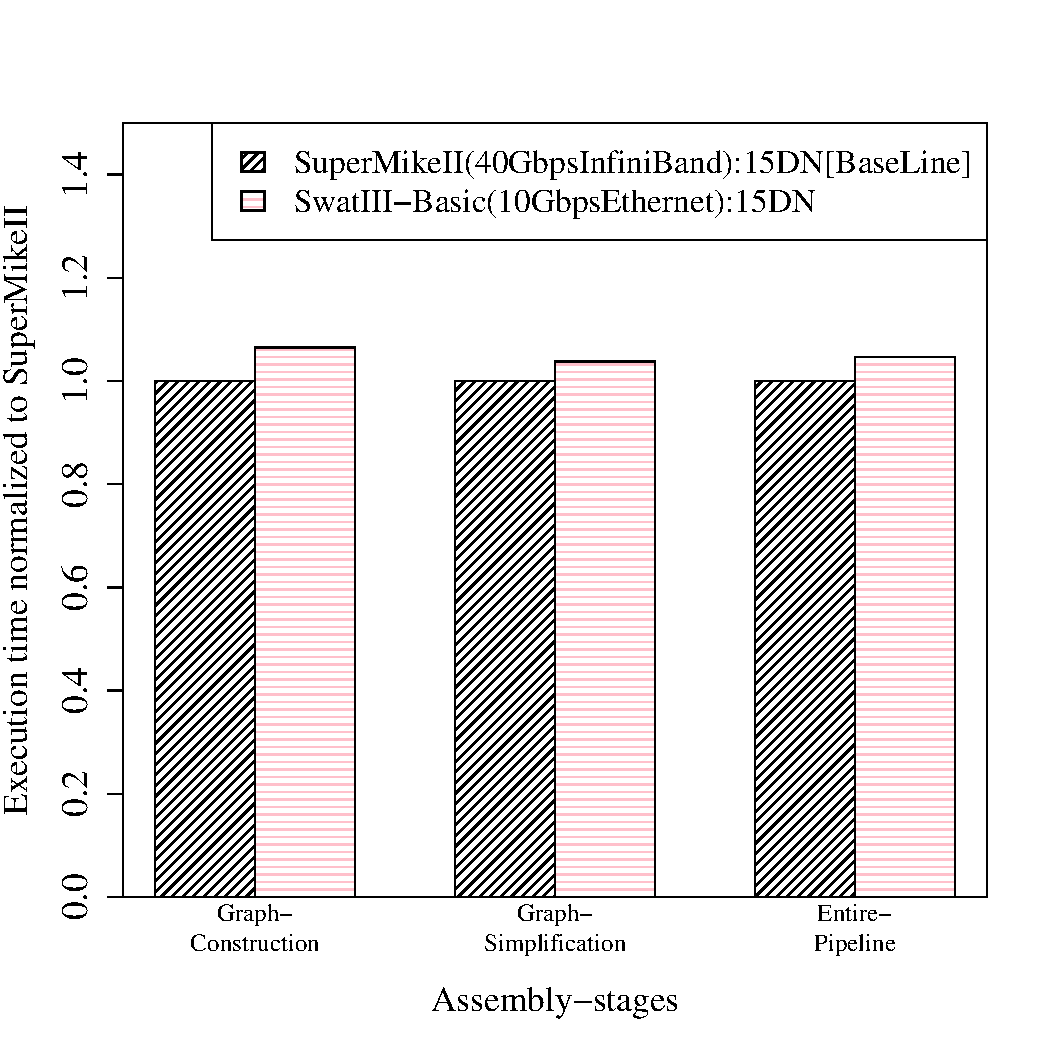
\includegraphics[width=\textwidth]{Figure/PerormanceData/Plots/Network.pdf}
                \caption{Effect of network}
                \label{fig:SuperMikeSwatBasic}
        \end{subfigure}
 	\begin{subfigure}[b]{0.23\textwidth}
                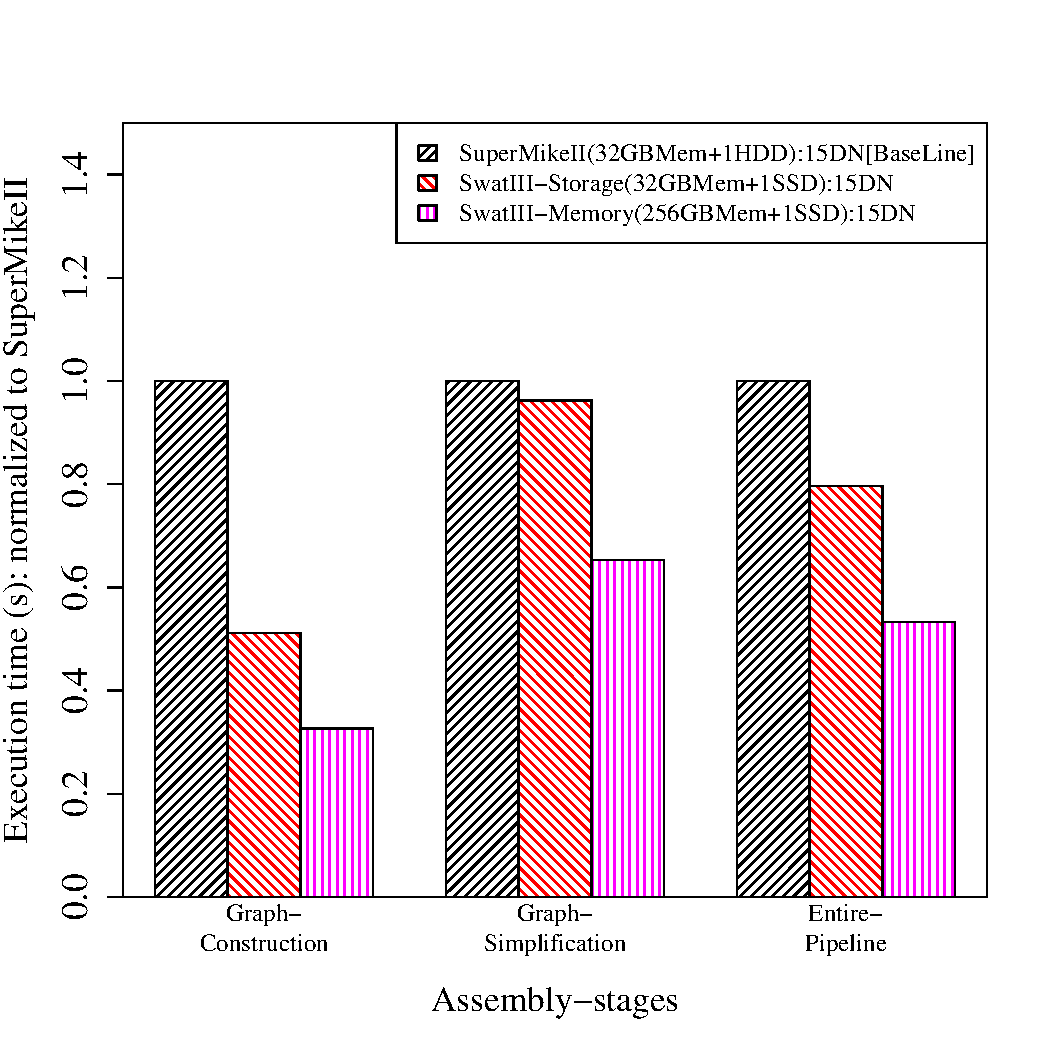
\includegraphics[width=\textwidth]{Figure/PerormanceData/Plots/StorageMemory.pdf}
                \caption{Effect of SSD and DRAM}
                \label{fig:SuperMikeSwatStorageMemory}
   \end{subfigure}
   \caption{Impact each individual hardware component on execution time of different stages of the assembly pipeline in 15 DataNodes }
  \label{fig:SuperMikeSwat}
\end{figure}

\subsection {Performance in SuperMikeII}
\label{PerformanceInSuperMikeII}
Since each node of SuperMikeII is equipped with only 1-HDD, there is a practical limitation on number of concurrently running yarn containers (hence, mappers and reducers) per node. 
More the number of mappers (or reducers) running simultaneously, more is the parallel disk-io especially during the shuffle phase. 
With only 1-HDD per node, the performance of Hadoop is advarsely affected because of huge amout of io-wait.
As a consequence, even if each node of SuperMikeII has 16 processing cores we observed the best performance for our entire assembly pipeline by running only 8 yarn-containers concurrently in each node, i.e. only half of the number of cores per node.

\subsection {Effect of Network} \label{EffectOfNetwork}
Figure-\ref{fig:SuperMikeSwatBasic} compares the impact of network interconnect on each stage of PGA's genome assembly pipeline while assembling a 90GB bumble bee genome. 
The execution time is normalized to the SuperMikeII-baseline. That is, the execution time on SuperMikeII for different stages of the asembler always have the value 1.
SuperMikeII uses a 40-Gbps QDR Infiniband whereas SwatIII-basic uses 10-Gbps ethernet. 
However, we did not find any visible performance difference (less than 2\%) on any of the stages of our assembly pipeline due to change in the network.
In order to investigate the reson in details, we measure the avaerage latency and the effective network-bandwith between two arbitrary compute nodes in SwatIII and SuperMikeII.
Since SuperMikeII uses an Infiniband connection the average latency was found to be more than 10-times lower compare to SwatIII which uses ethernet.
The avarage latency in SuperMikeII was found to be $.014$ms whereas in SwatIII, it is almost $0.2$ms.
However, due to the resource sharing among many users, the average effective-bandwith of SuperMikeII was found to be almost 10-times lower than that of SwatIII: 949Mbit/s in SuperMikeII, whereas 9.1Gbit/s in SwatIII.
Furthermore, the java-based APIs of Hadoop or Giraph is not optimized to take the advantage of Infiniband. 
Hence, in any of the Hadoop or Giraph workloads in the moderate size bumble bee genome assembly pipeline we did not observe major performance difference using same number of nodes in SwatIII.
 

%Although there was no visible difference in the execution-time for both the network in case of the best performance in our assembly, we experimented with the a varying number of concurrently running yarn-containers (i.e. number of mappers, reducers or Giraph-workers). 
%In case of a Giraph job we observed an almost exponential increase in the number of TCP connections with increase in number of Giraph-workers. Figure-\ref{fig:GiraphTCP} shows the increase in number of TCP connections when we increase the number of Giraph workers from 115 to 220 as shown in the Figure-GiraphTcp.
\begin{figure*}[htb]
%\centering
        \begin{subfigure}[b]{0.23\textwidth}
                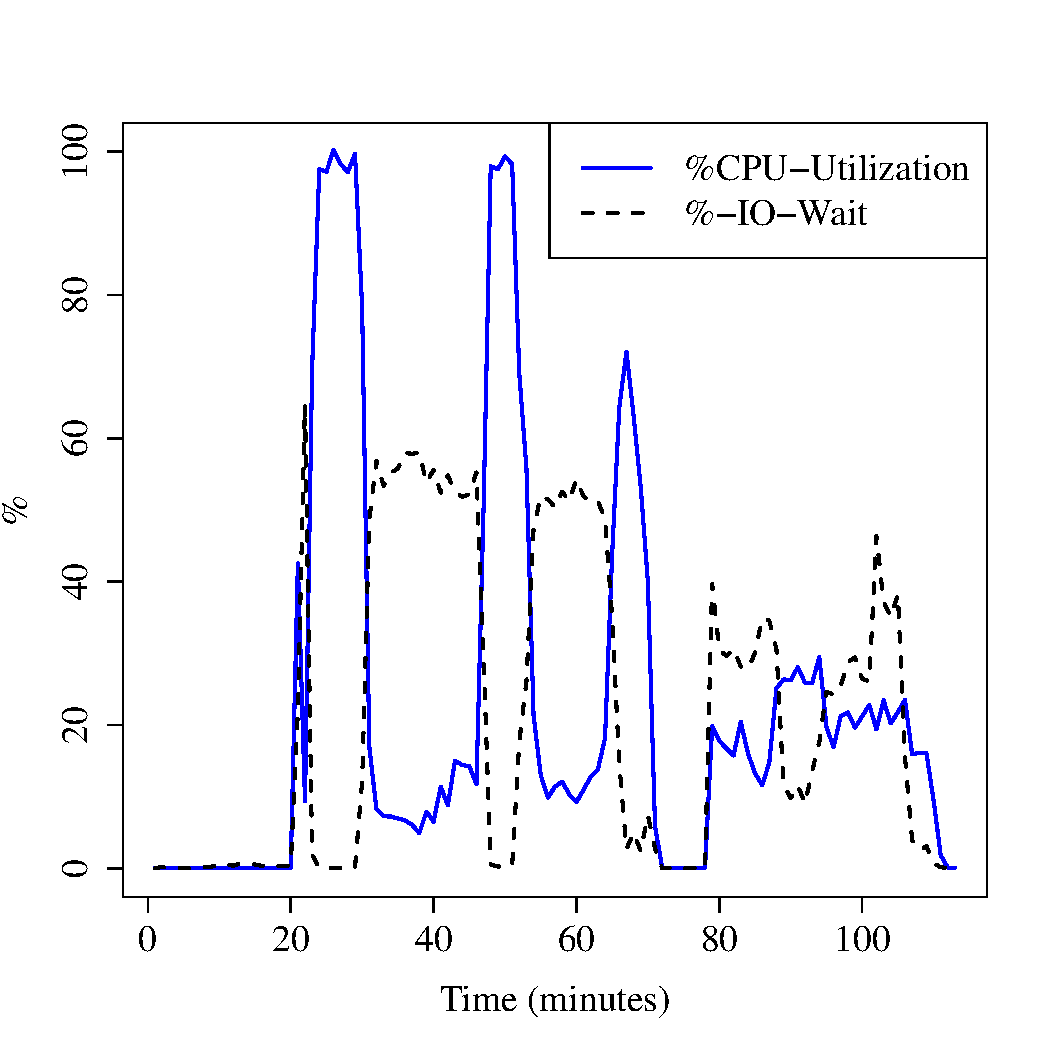
\includegraphics[width=\textwidth]{Figure/SystemData/Plots/BGCPUHDD.pdf}
                \caption{Graph Construction in SwatIII-Basic}
                \label{fig:BGCPUHDD}
        \end{subfigure}
		\begin{subfigure}[b]{0.23\textwidth}
                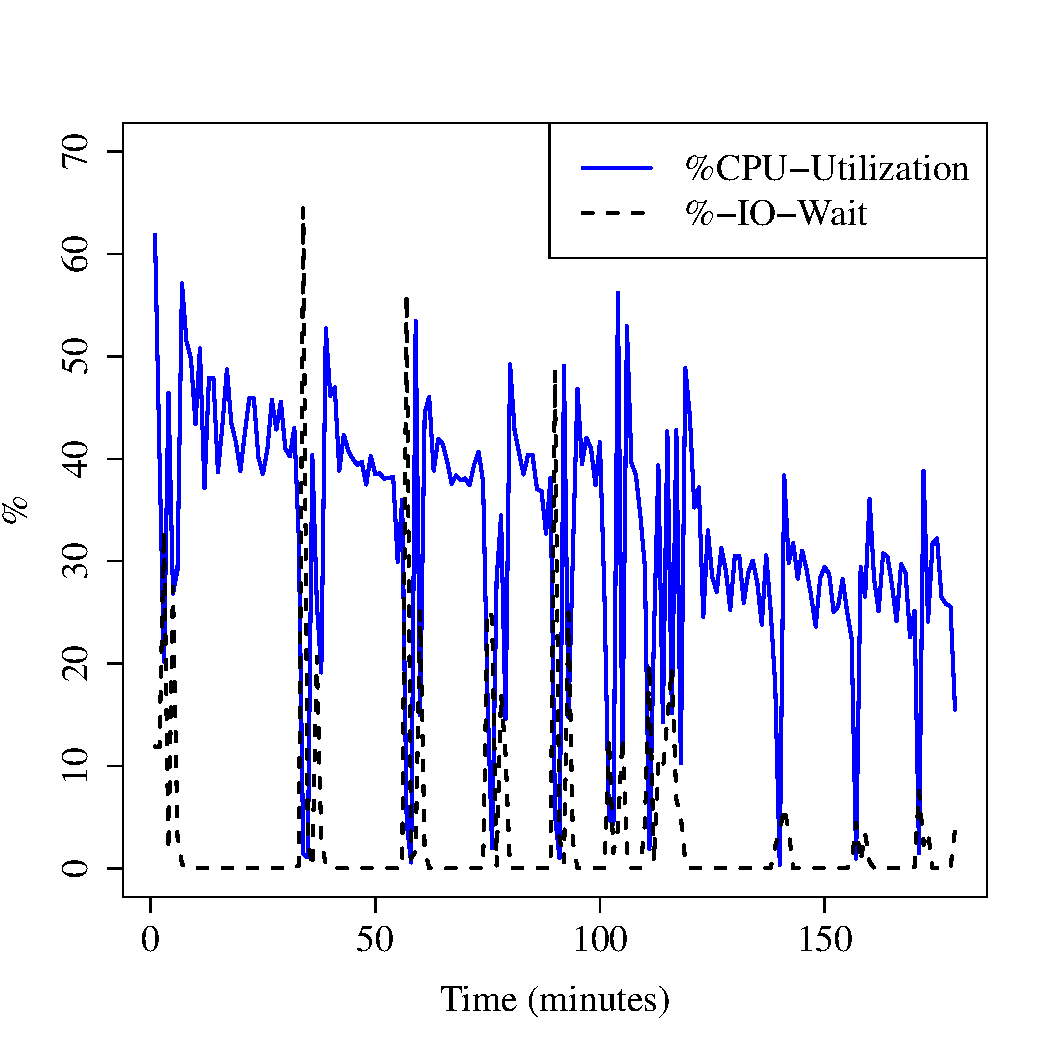
\includegraphics[width=\textwidth]{Figure/SystemData/Plots/ECCPUHDD.pdf}
                \caption{Graph Simplification in SwatIII-Basic}
                \label{fig:ECCPUHDD}
        \end{subfigure} 
        %\begin{subfigure}[b]{0.3\textwidth}
        %        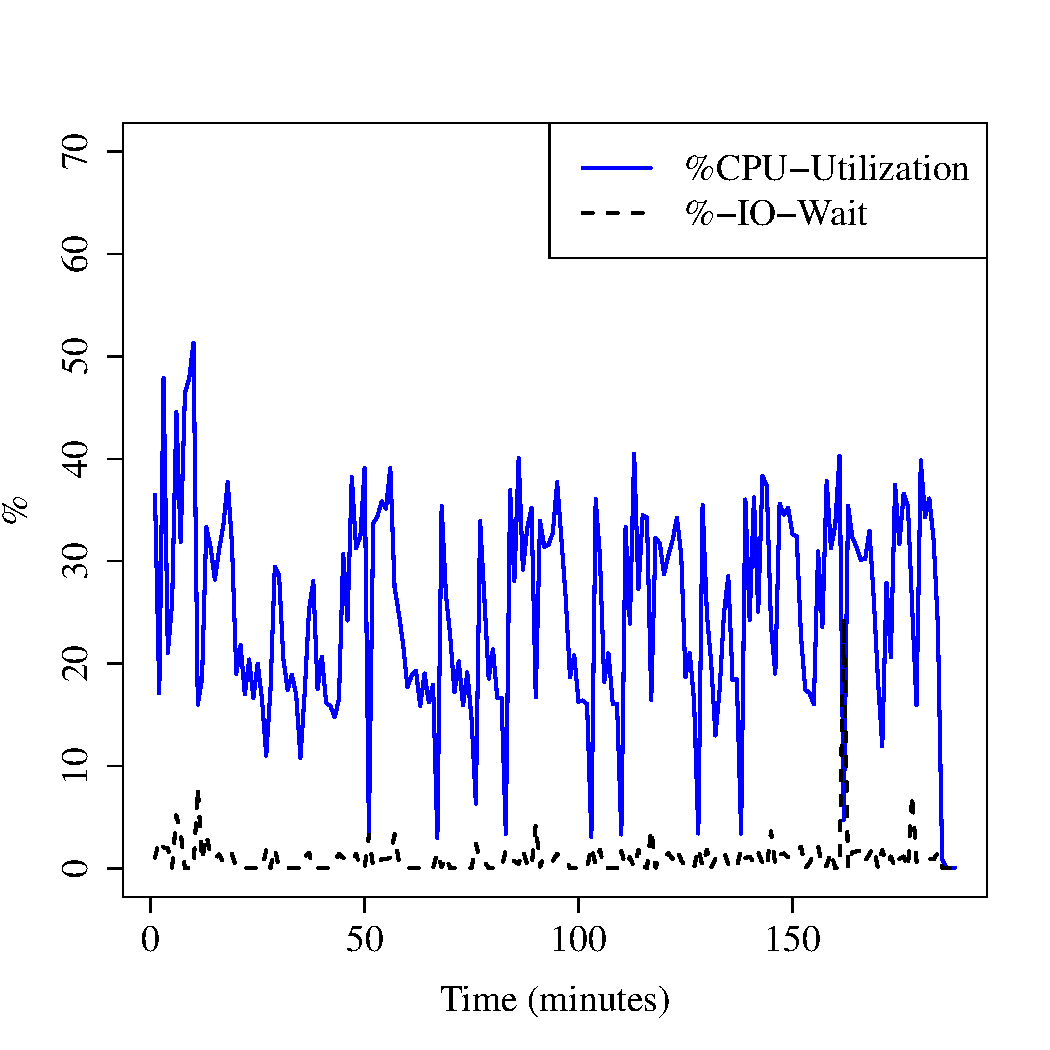
\includegraphics[width=\textwidth]{Figure/SystemData/Plots/SCFCPUHDD.pdf}
        %        \caption{Scaffolding in SwatIII-Basic}
        %        \label{fig:SCFCPUHDD}
        %\end{subfigure}       
        \begin{subfigure}[b]{0.23\textwidth}
                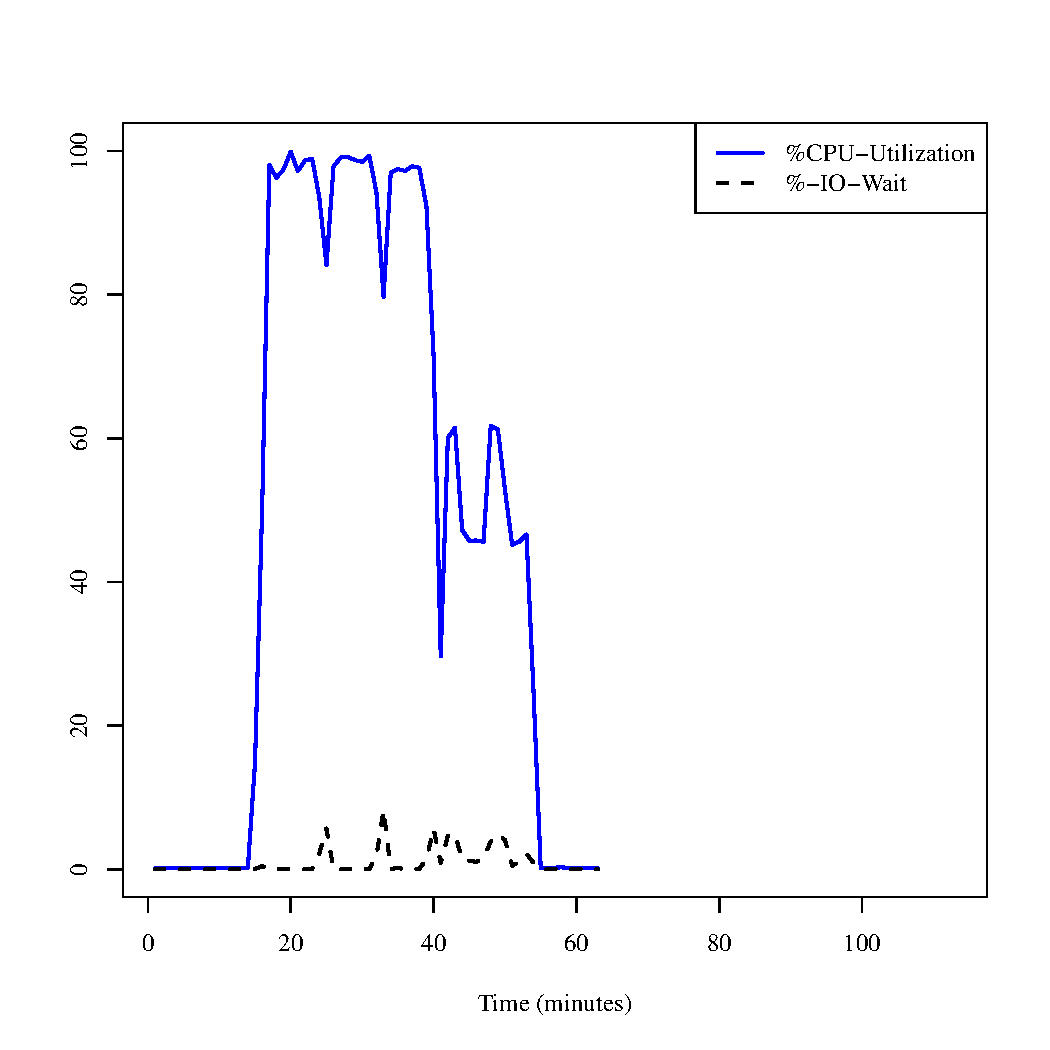
\includegraphics[width=\textwidth]{Figure/SystemData/Plots/BGCPUSSD.pdf}
                \caption{Graph Construction in SwatIII-Storage}
                \label{fig:BGCPUSSD}
        \end{subfigure}    
        \begin{subfigure}[b]{0.23\textwidth}
                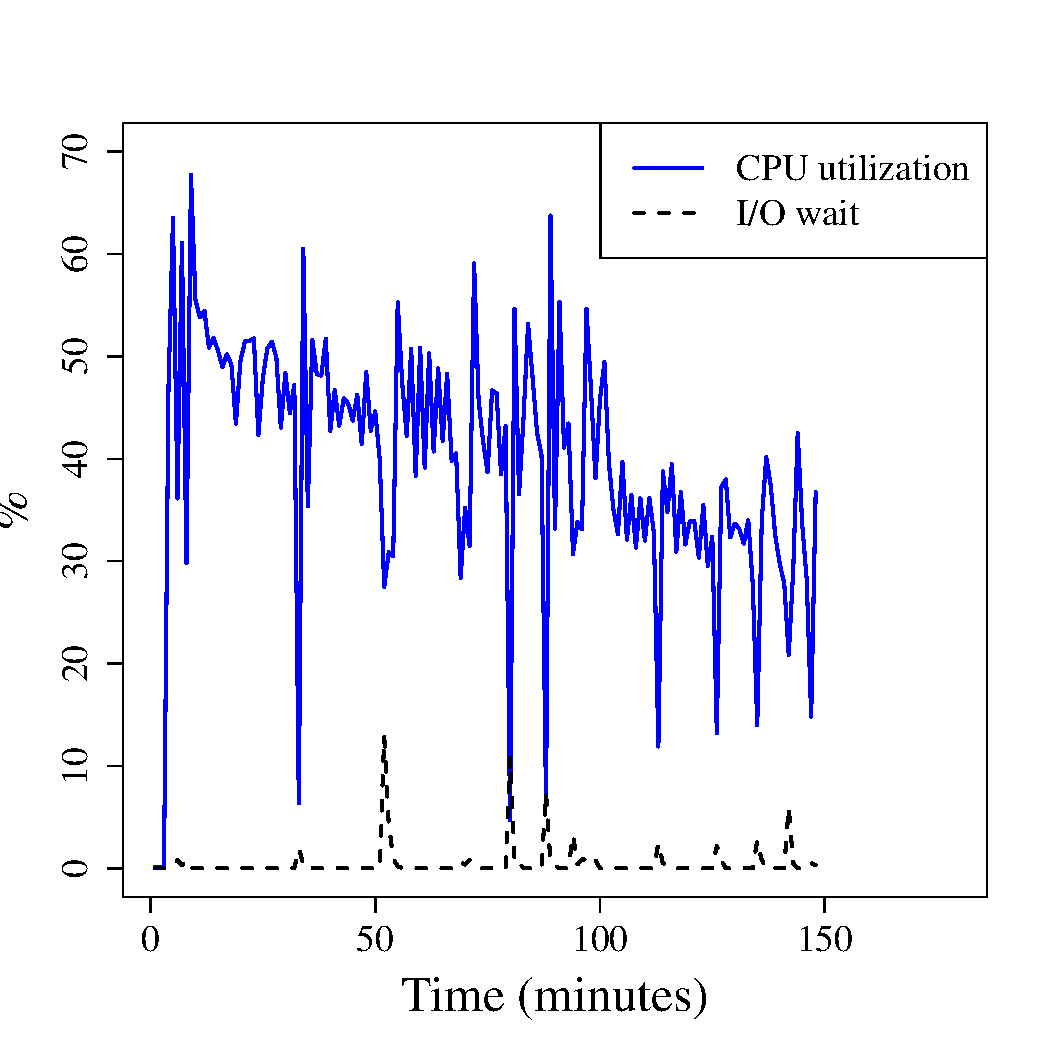
\includegraphics[width=\textwidth]{Figure/SystemData/Plots/ECCPUSSD.pdf}
                \caption{Graph Simplification in SwatIII-Storage}
                \label{fig:ECCPUSSD}
        \end{subfigure}
        %\begin{subfigure}[b]{0.3\textwidth}
        %        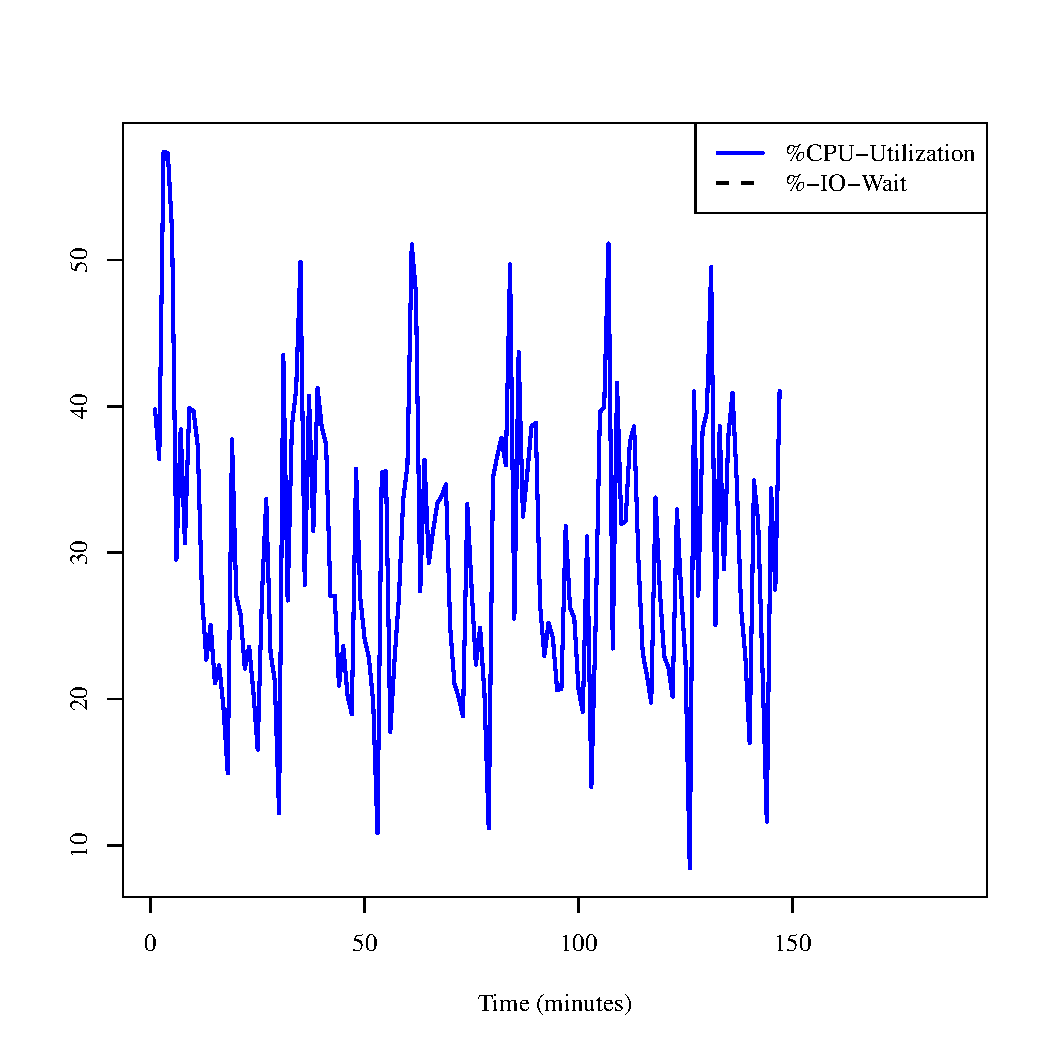
\includegraphics[width=\textwidth]{Figure/SystemData/Plots/SCFCPUSSD.pdf}
        %        \caption{Scaffolding in SwatIII-Storage}
        %        \label{fig:SCFCPUSSD}
        %\end{subfigure}
        \caption{CPU-Utilization and IO-Wait characteristics in SwatIII-Basic (1-HDD/node) and SwatIII-Storage(1-SSD/node)}\label{fig:HddSsdCPU}
\end{figure*}

\begin{figure*}[htb]
%        \centering
%        \begin{subfigure}[b]{0.3\textwidth}
%                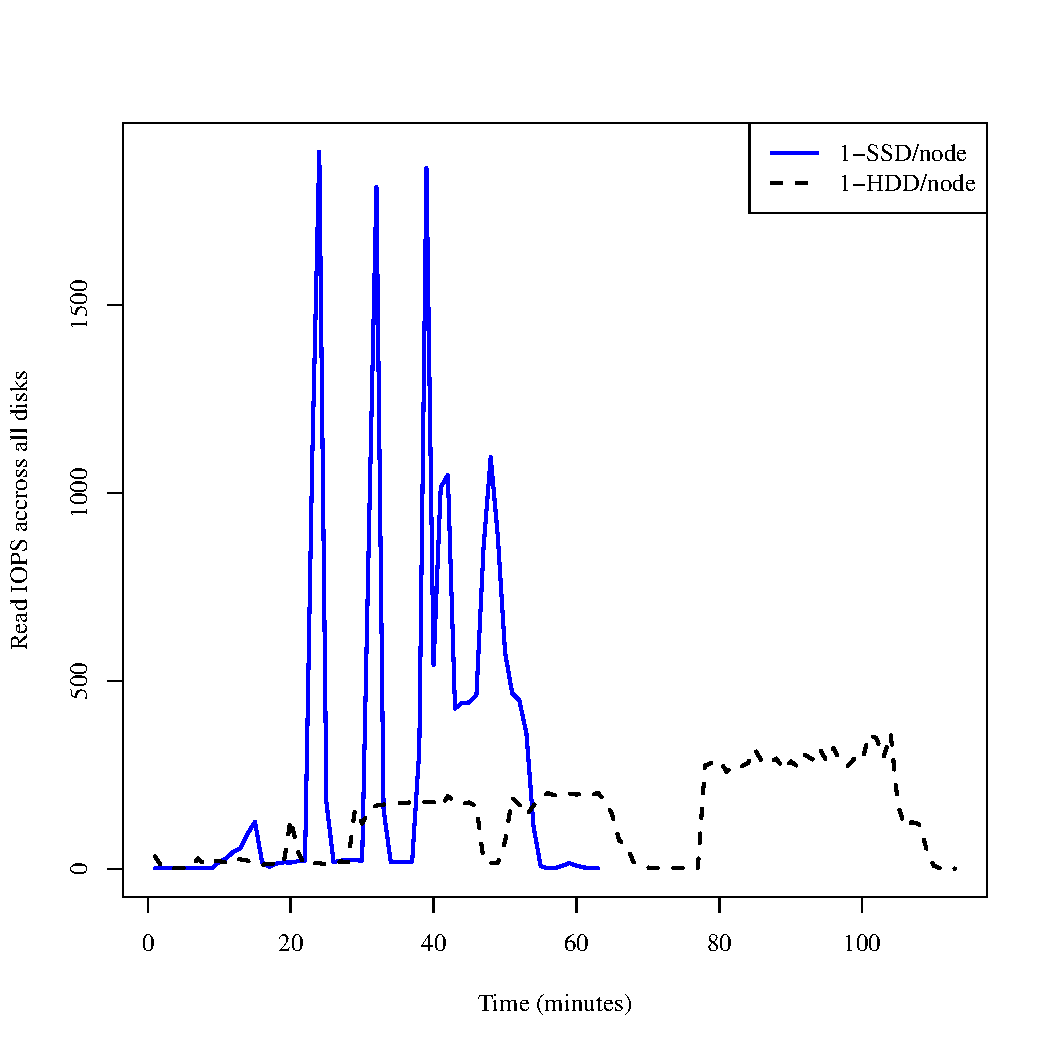
\includegraphics[width=\textwidth]{Figure/SystemData/Plots/BGHddSsdRdIops.pdf}
%                \caption{Read-Iops in Graph Construction in SwatIII-Basic and SwatIII-Storage}
%                \label{fig:BGHddSsdRdIops}
%        \end{subfigure}
%        ~ %add desired spacing between images, e. g. ~, \quad, \qquad, \hfill etc.
%          %(or a blank line to force the subfigure onto a new line)
%        \begin{subfigure}[b]{0.3\textwidth}
%                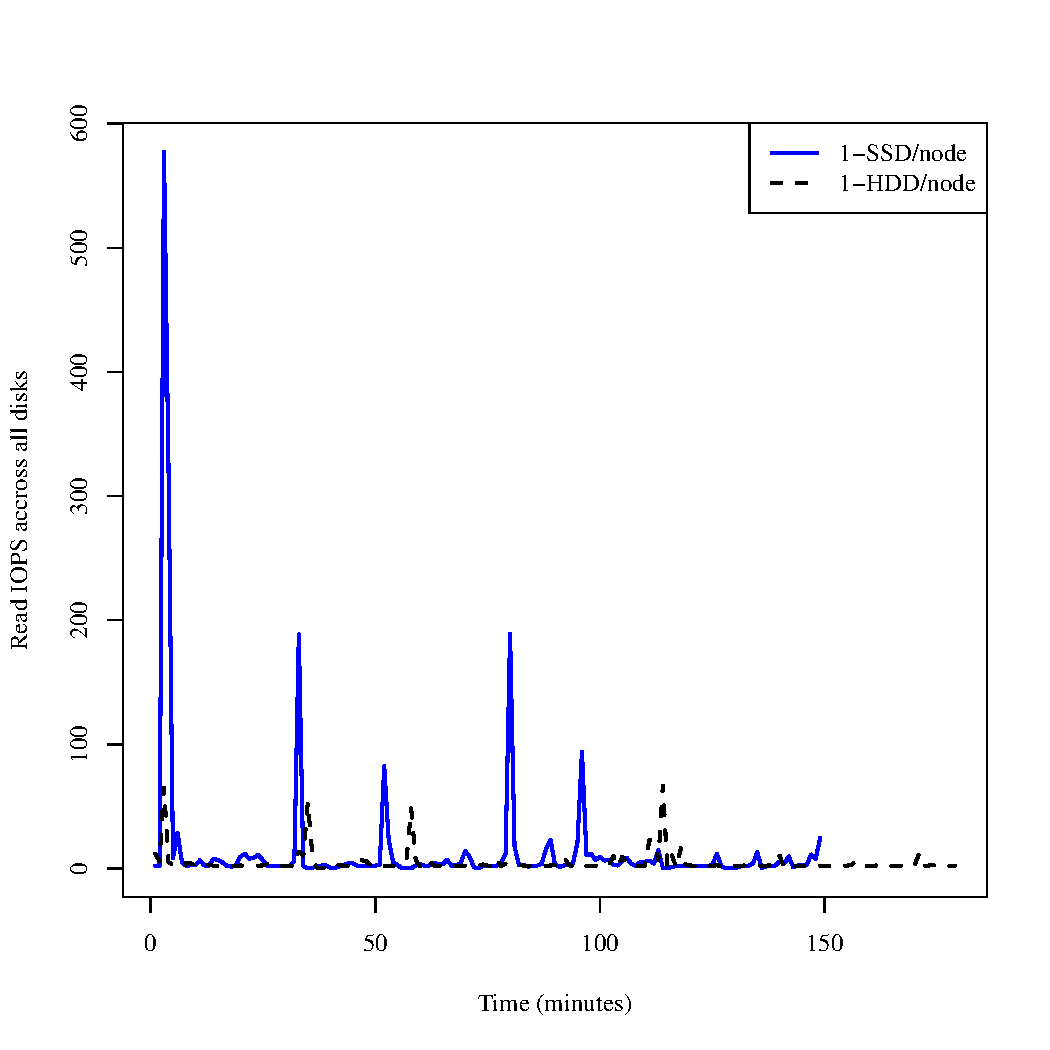
\includegraphics[width=\textwidth]{Figure/SystemData/Plots/ECHddSsdRdIops.pdf}
%                \caption{Read-Iops in Graph Simplification in SwatIII-Basic and SwatIII-Storage}
%                \label{fig:ECHddSsdRdIops}
%        \end{subfigure}
%        ~ %add desired spacing between images, e. g. ~, \quad, \qquad, \hfill etc.
%          %(or a blank line to force the subfigure onto a new line)
%        \begin{subfigure}[b]{0.3\textwidth}
%                \includegraphics[width=\textwidth]%{Figure/SystemData/Plots/SCFHddSsdRdIops.pdf}
%                \caption{Read-Iops in Scaffolding in SwatIII-Basic and SwatIII-Storage}
%                \label{fig:SCFHddSsdRdIops}
%        \end{subfigure}        
        \begin{subfigure}[b]{0.23\textwidth}
                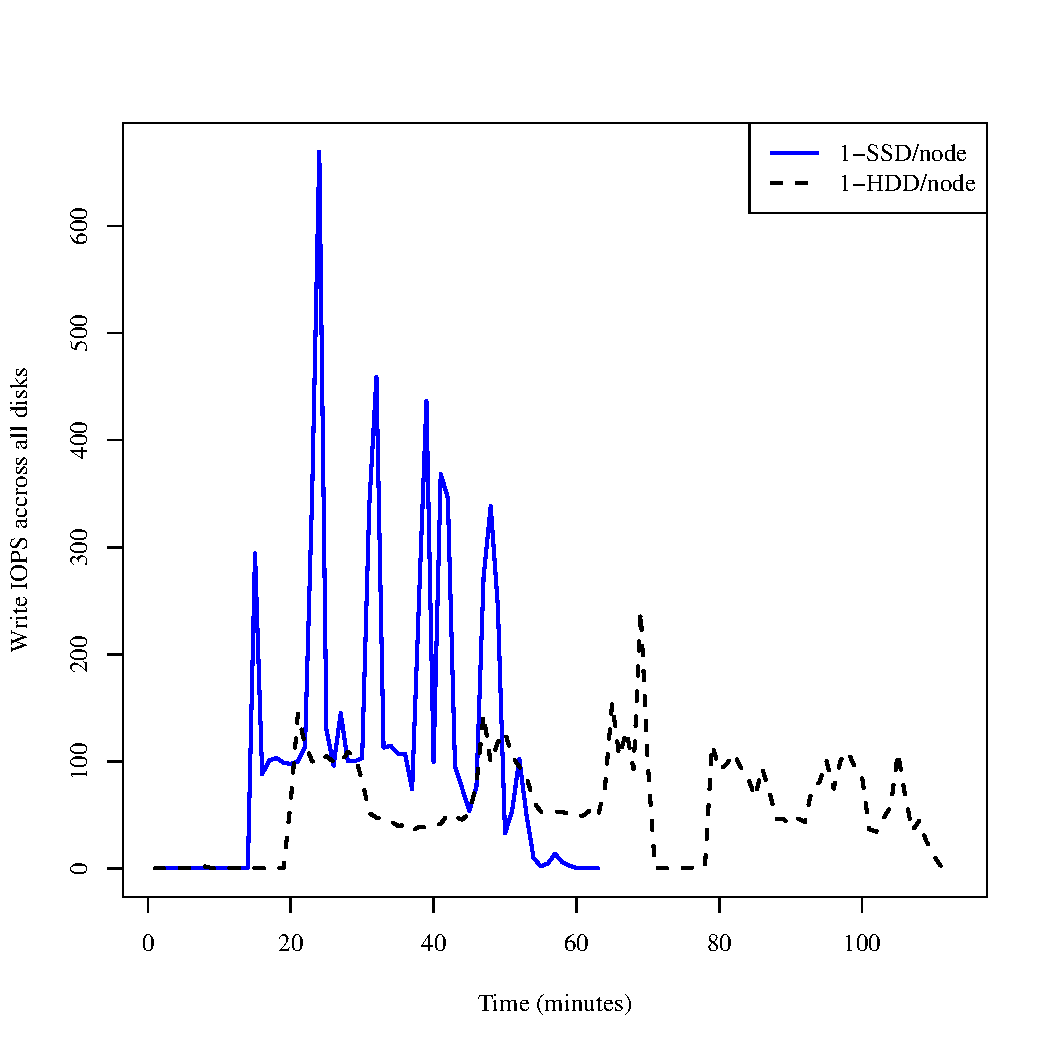
\includegraphics[width=\textwidth]{Figure/SystemData/Plots/BGHddSsdWrIops.pdf}
                \caption{Write-Iops in Graph Construction in SwatIII-Basic and SwatIII-Storage}
                \label{fig:BGHddSsdWrIops}
        \end{subfigure}
        ~ %add desired spacing between images, e. g. ~, \quad, \qquad, \hfill etc.
          %(or a blank line to force the subfigure onto a new line)
        \begin{subfigure}[b]{0.23\textwidth}
                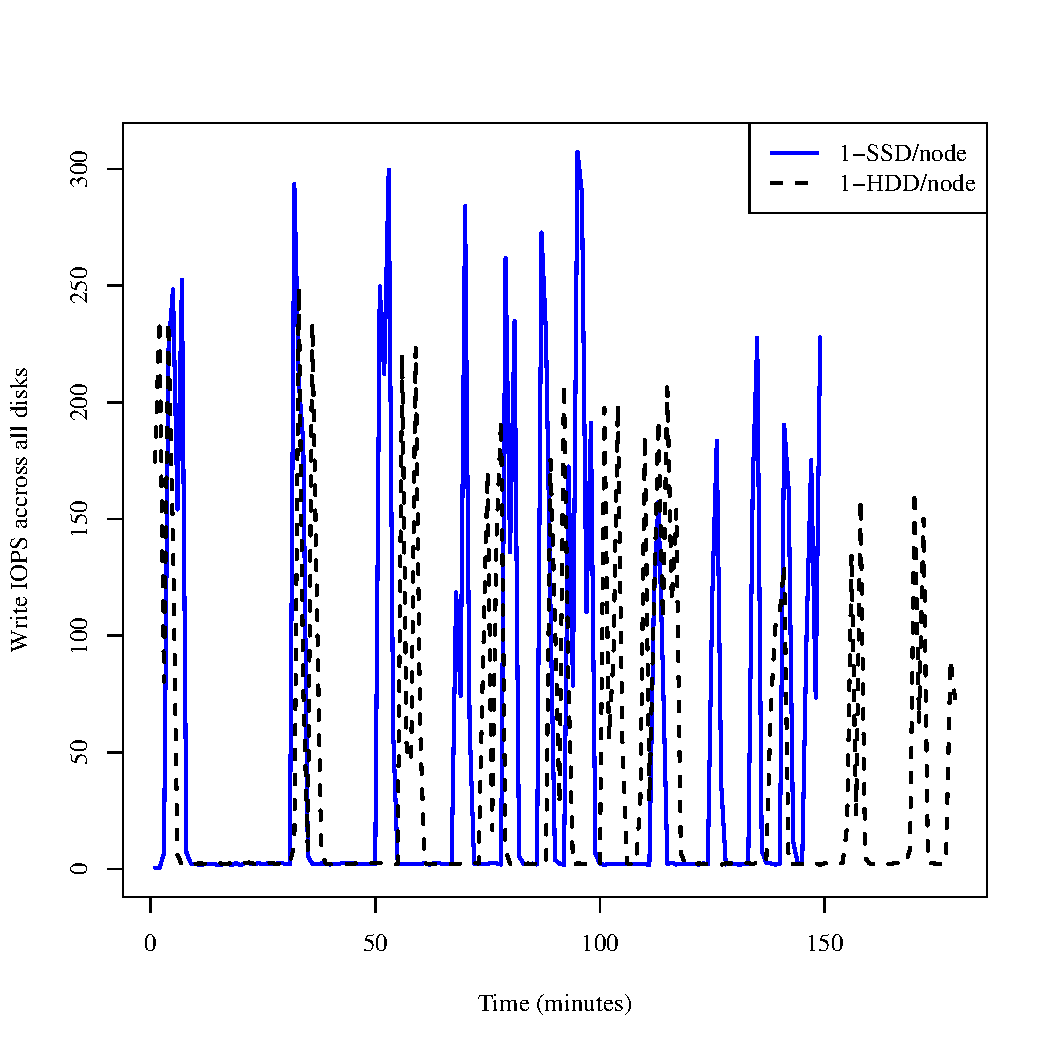
\includegraphics[width=\textwidth]{Figure/SystemData/Plots/ECHddSsdWrIops.pdf}
                \caption{Write-Iops in Graph Simplification in SwatIII-Basic and SwatIII-Storage}
                \label{fig:ECHddSsdWrIops}
        \end{subfigure}
        ~ %add desired spacing between images, e. g. ~, \quad, \qquad, \hfill etc.
          %(or a blank line to force the subfigure onto a new line)
        %\begin{subfigure}[b]{0.3\textwidth}
        %        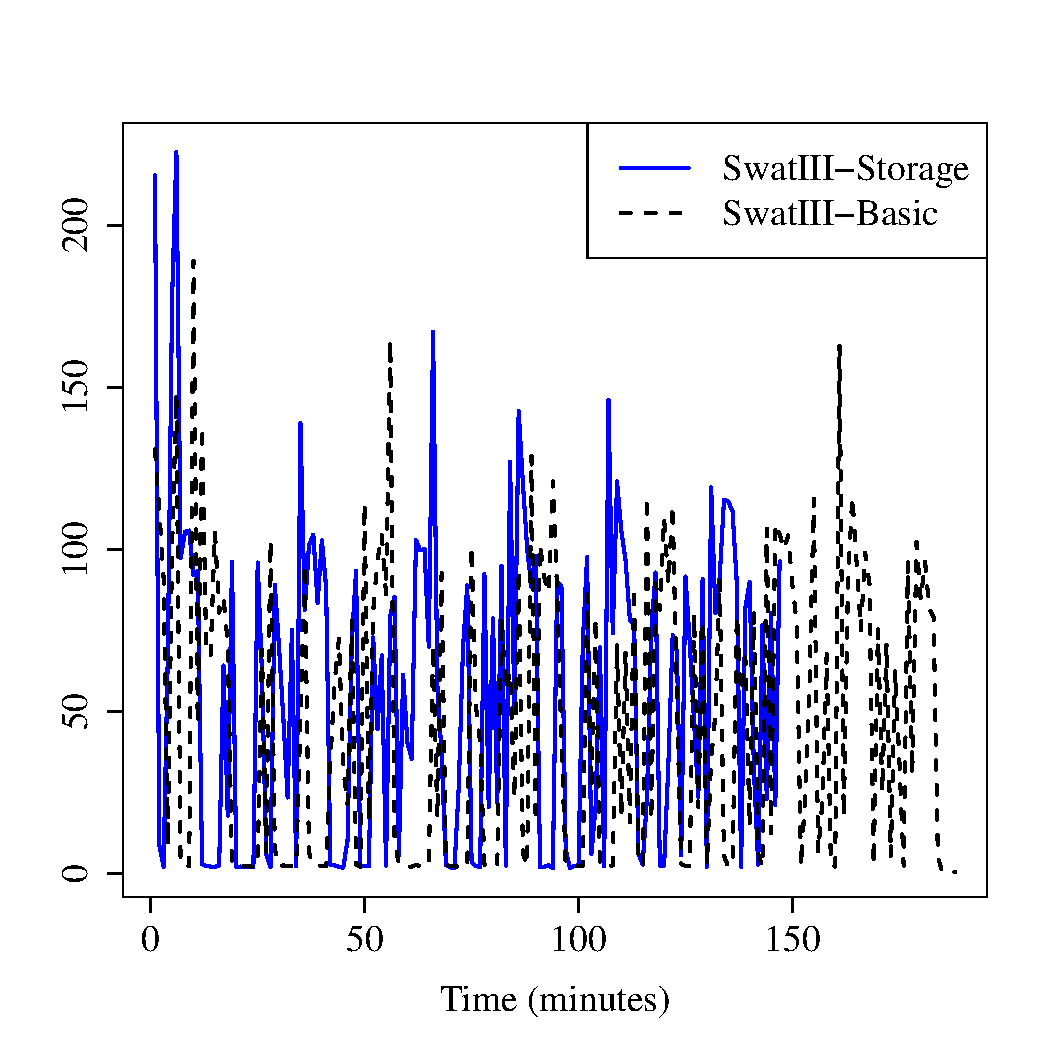
\includegraphics[width=\textwidth]{Figure/SystemData/Plots/SCFHddSsdWrIops.pdf}
        %        \caption{Write-Iops in Scaffolding in SwatIII-Basic and SwatIII-Storage}
         %       \label{fig:SCFHddSsdWrIops}
        %\end{subfigure}
	%\caption{Comparison of Total Write-IOPS in one host in SwatIII-Basic (1-HDD/node) and SwatIII-Storage (1-SSD/node)} \label{fig:HddSsdRWiops}
%\end{figure*}
%\begin{figure*}[htb]
%        \centering
%        \begin{subfigure}[b]{0.3\textwidth}
%                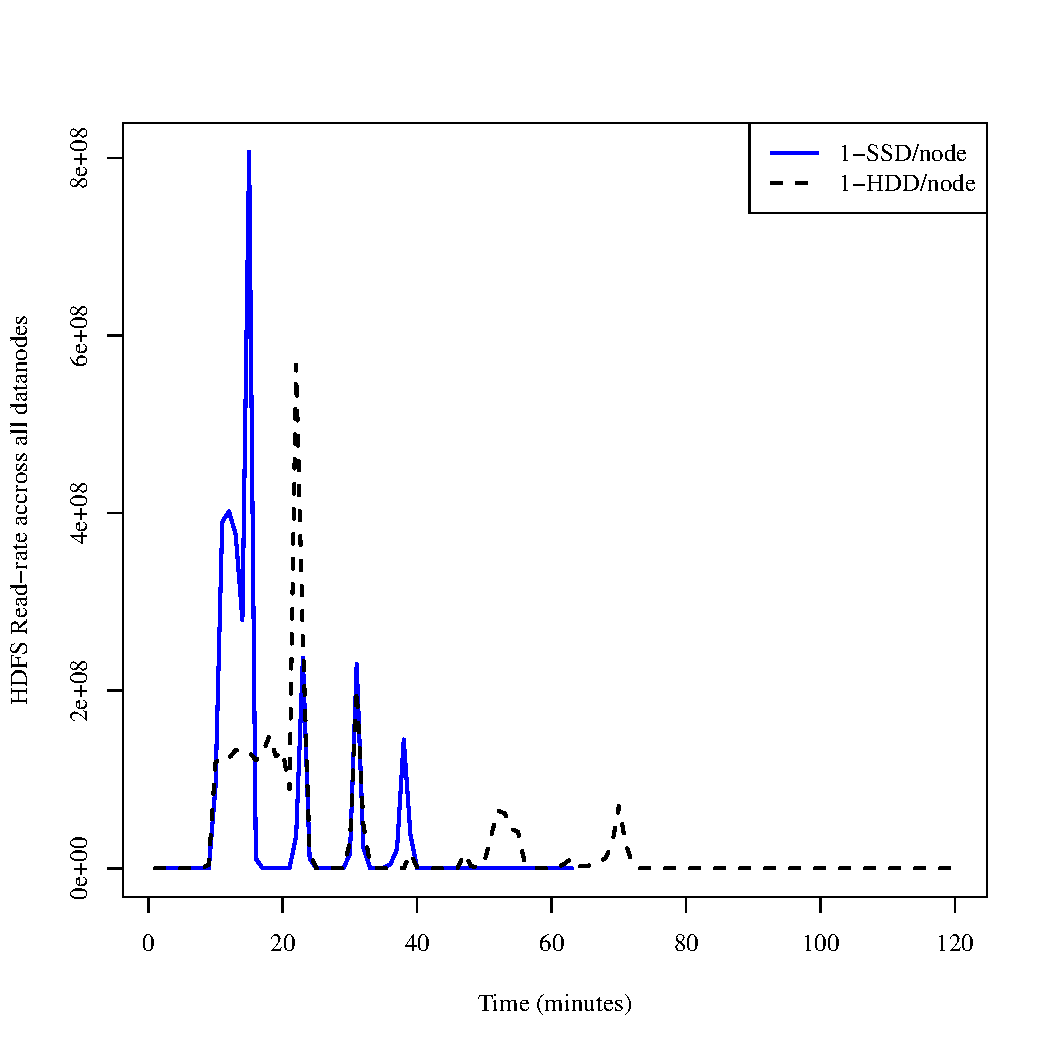
\includegraphics[width=\textwidth]{Figure/SystemData/Plots/BGHddSsdHdfsRdIops.pdf}
%                \caption{HDFS-Read-Rate in Graph Construction in SwatIII-Basic and SwatIII-Storage}
%                \label{fig:BGHddSsdHdfsRdIops}
%        \end{subfigure}
%        ~ %add desired spacing between images, e. g. ~, \quad, \qquad, \hfill etc.
%          %(or a blank line to force the subfigure onto a new line)
%        \begin{subfigure}[b]{0.3\textwidth}
%                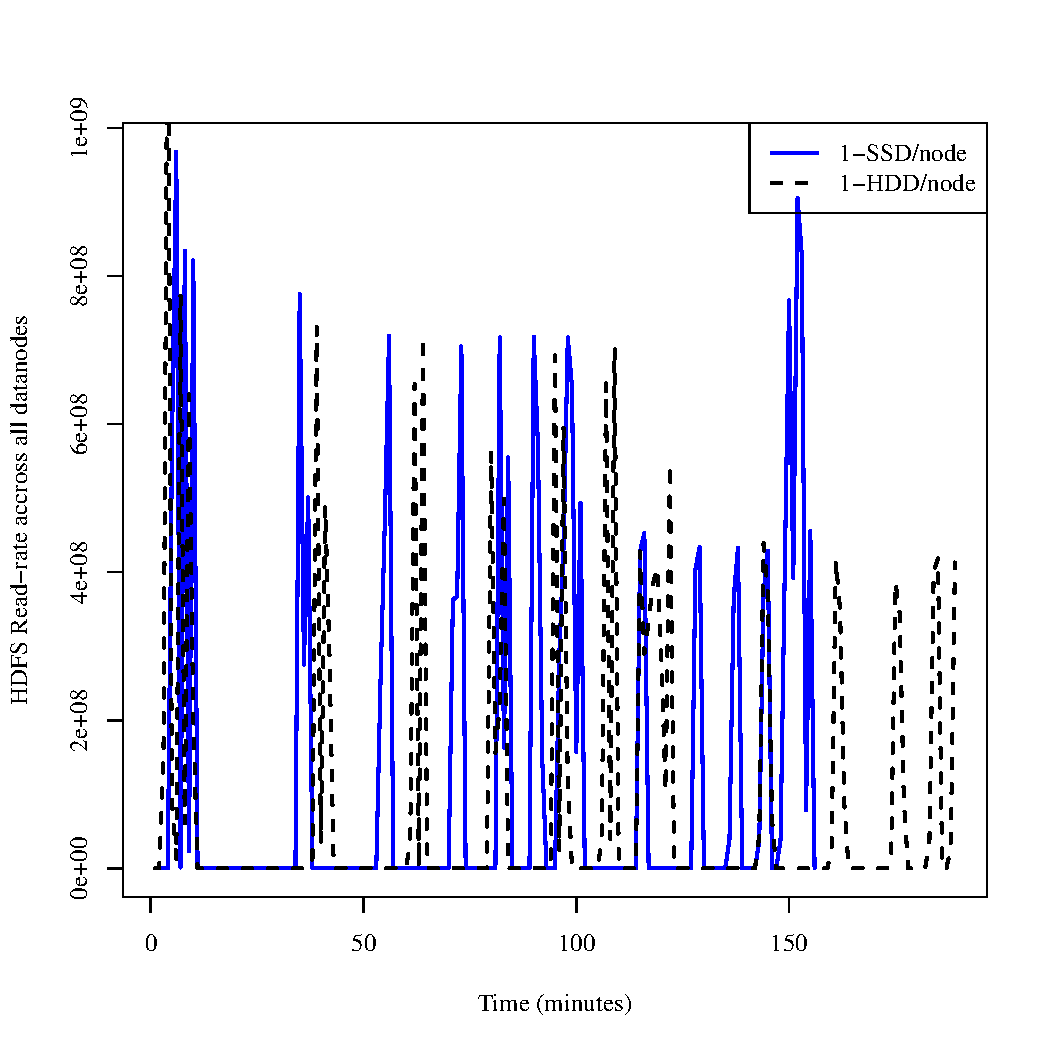
\includegraphics[width=\textwidth]{Figure/SystemData/Plots/ECHddSsdHdfsRdIops.pdf}
%                \caption{HDFS-Read-Rate in Graph Simplification in SwatIII-Basic and SwatIII-Storage}
%                \label{fig:ECHddSsdHdfsRdIops}
%        \end{subfigure}
%        ~ %add desired spacing between images, e. g. ~, \quad, \qquad, \hfill etc.
%          %(or a blank line to force the subfigure onto a new line)
%        \begin{subfigure}[b]{0.3\textwidth}
%                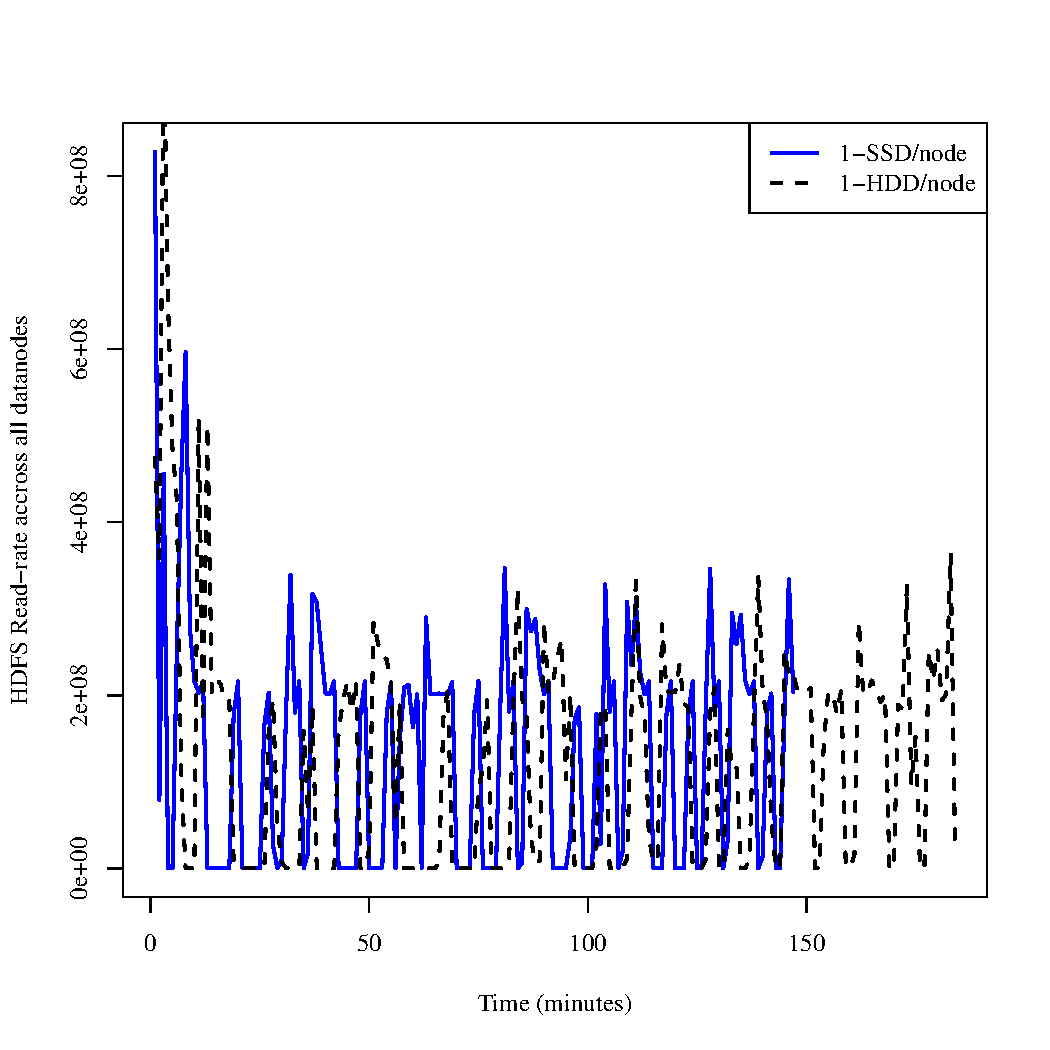
\includegraphics[width=\textwidth]{Figure/SystemData/Plots/SCFHddSsdHdfsRdIops.pdf}
%                \caption{HDFS-Read-Rate in Scaffolding phase in SwatIII-Basic and SwatIII-Storage}
%                \label{fig:SCFHddSsdHdfsRdIops}
%        \end{subfigure}        
        \begin{subfigure}[b]{0.23\textwidth}
                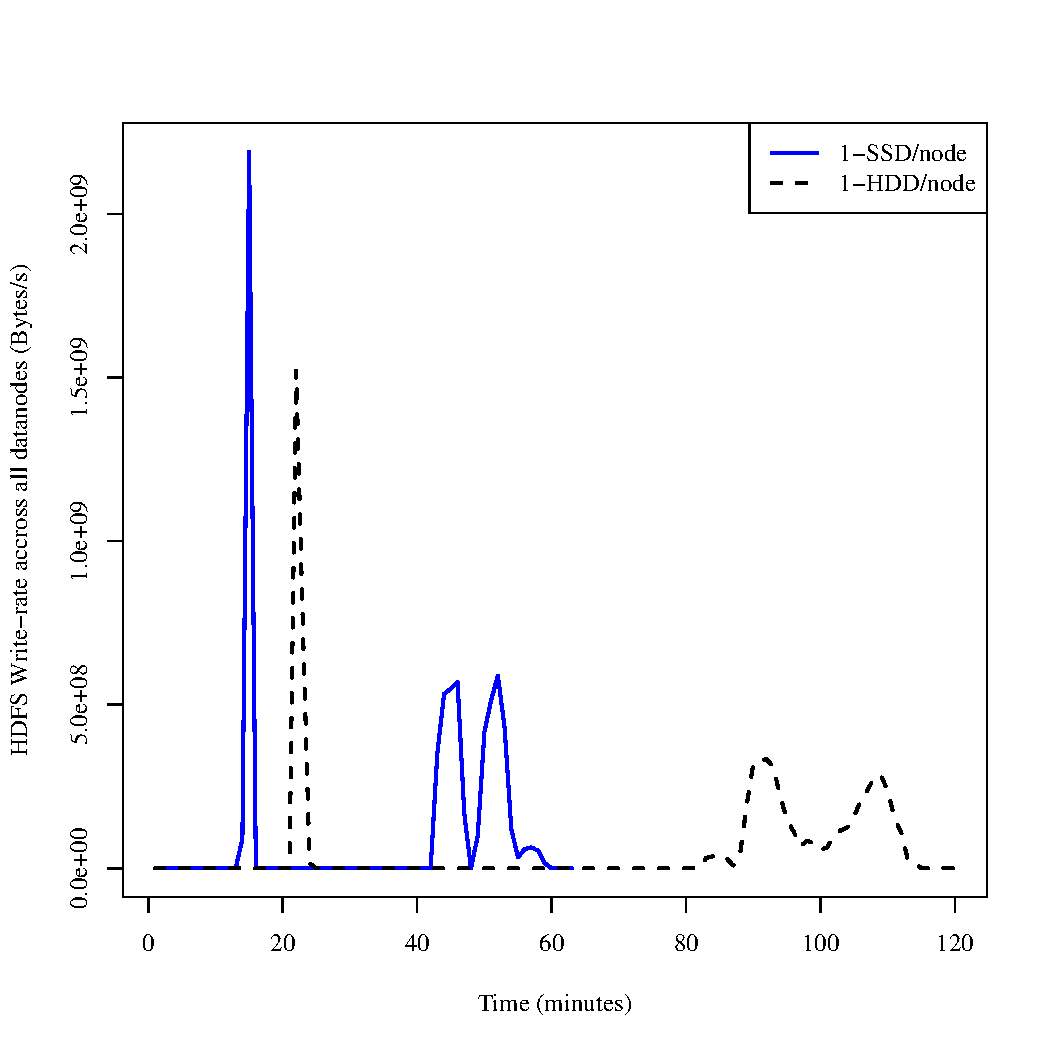
\includegraphics[width=\textwidth]{Figure/SystemData/Plots/BGHddSsdHdfsWrIops.pdf}
                \caption{HDFS-Write-Rate in Graph Construction in SwatIII-Basic and SwatIII-Storage}
                \label{fig:BGHddSsdHdfsWrIops}
        \end{subfigure}
        ~ %add desired spacing between images, e. g. ~, \quad, \qquad, \hfill etc.
          %(or a blank line to force the subfigure onto a new line)
        \begin{subfigure}[b]{0.23\textwidth}
                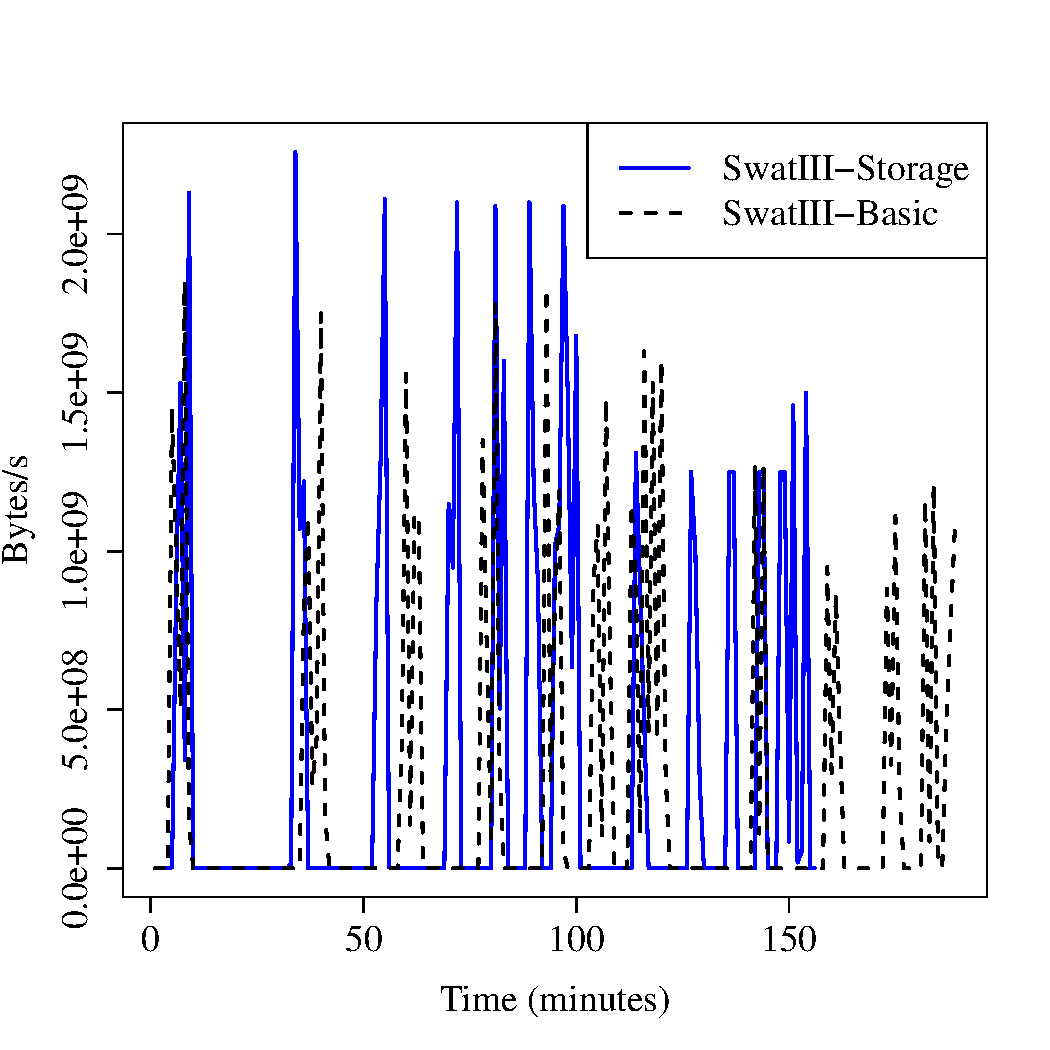
\includegraphics[width=\textwidth]{Figure/SystemData/Plots/ECHddSsdHdfsWrIops.pdf}
                \caption{HDFS-Write-Rate in Graph Simplification in SwatIII-Basic and SwatIII-Storage}
                \label{fig:ECHddSsdHdfsWrIops}
        \end{subfigure}
        ~ %add desired spacing between images, e. g. ~, \quad, \qquad, \hfill etc.
          %(or a blank line to force the subfigure onto a new line)
        %\begin{subfigure}[b]{0.3\textwidth}
        %        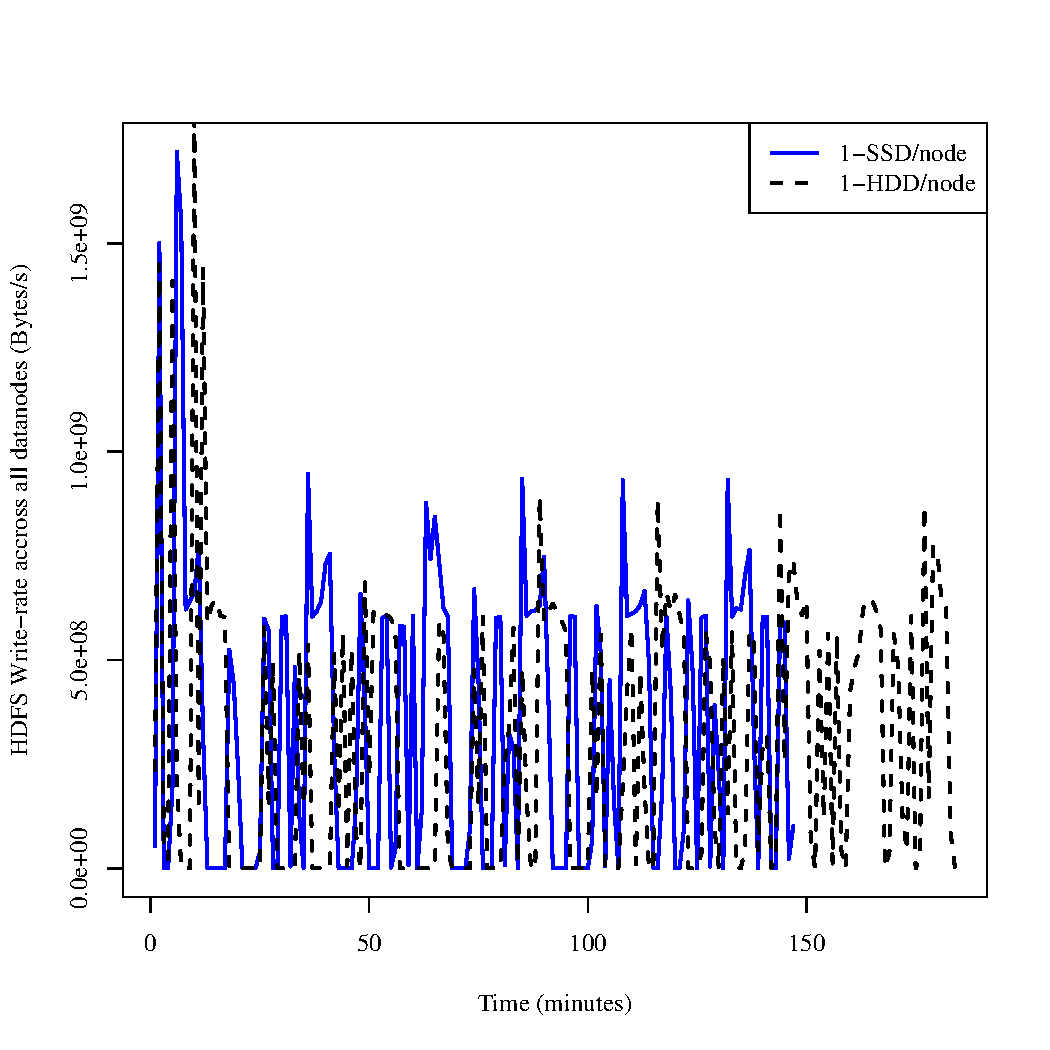
\includegraphics[width=\textwidth]{Figure/SystemData/Plots/SCFHddSsdHdfsWrIops.pdf}
        %        \caption{HDFS-Write-Rate in Scaffolding phase in SwatIII-Basic and SwatIII-Storage}
        %        \label{fig:SCFHddSsdHdfsWrIops}
        %\end{subfigure}        
        \caption{Comparison of rate of disk write on Local File System (of one datanode) and HDFS (across all datanodes) SwatIII-Basic (1-HDD/node) and SwatIII-Storage (1-SSD/node)}\label{fig:HddSsdHdfsRWps}
        
\end{figure*}
\subsection {Effect of SSD} \label{EffectOfSSD}
Figure-\ref{fig:SuperMikeSwatStorageMemory} compares the execution time of SwatIII-Storage (1-SSD/node) to the SuperMikeII-baseline (1-HDD/node).
%The execution time is again normalized to the SuperMikeII-baseline.
The second column of each stage of the assembler in Figure-\ref{fig:SuperMikeSwat} shows the impact of using SSD in that stage of the assembly.
%Graph construction being a shuffle-intensive Hadoop job, got maximum benefit from SSD. 
We observed almost 50\% improvement in the shuffle intensive graph-construction stage because of reduced io-wait. 
However, graph-simplification, being a series of in-memory Giraph jobs is not affected much (less than 5\%) by storage optimization with SSD. 
%Scaffolding stage, being a mix of small Hadoop and Giraph job the corresponding gain is almost 10\%.

Figure-\ref{fig:HddSsdCPU} compares the CPU-utilization and IO-wait characteristics for 1-HDD and 1-SSD per node.
%As mentioned earlier, for any map-reduce job we always started the reducers after all the mappers finished. 
%The first three peaks in the left side of figure-\ref{fig:BGCPUHDD} and \ref{fig:BGCPUSSD} corresponds to the CPU utilization during three mapper-waves. 
The performance of a shuffle-intensive Hadoop job becomes io-bound mainly in two places. First, at the end of each mapper-wave when many mappers write intermediate shuffle data parallely to the local file system. Second, when this shuffled data is read by the reducers.
A Giraph job becomes io-bound when it reads/writes a large graph from/to HDFS as shown in figure-\ref{fig:ECCPUHDD}.
%Scaffolding being a series of small Hadoop and Giraph job suffers from least io-wait. 
As shown in figure-\ref{fig:BGCPUSSD} and \ref{fig:ECCPUSSD} io-wait is reduced by using solid state drive (SSD) instead of HDD. 

Basically the SSD increases the disk io-rate tremendously especially in case of the local file system that is the shuffle phase of Hadoop.
Figure-\ref{fig:BGHddSsdWrIops} shows that SSD improves the peak IOPS 7 to 8 times in one of the datanodes than corresponding HDD case during the shuffle phase of the Hadoop build-graph job.
On the other hand, figure-\ref{fig:ECHddSsdWrIops} compares the rate of local disk-write of the same datanode for a series of Giraph jobs which read/write only to the HDFS.
Whereas, figure-\ref{fig:BGHddSsdHdfsWrIops} and  \ref{fig:ECHddSsdHdfsWrIops} shows the write rate over HDFS across all datanodes.
From the later three cases, the SSD is found to yield 2-times improvement in the peak HDFS read/write.
%Figure-\ref{fig:BGHddSsdWrIops} and \ref{fig:ECHddSsdWrIops} compares the read and write io operations per second to the local disk (of one datanode) for different stages of the same assembly using HDD and SSD.
%We observed almost 7 to 8 times improvement in the peak IOPS in case of SSD than HDD in the shuffle-intensive graph construction phase that writes huge amount of data to the local file system.
%Figure-\ref{fig:HddSsdHdfsRWps} compares the total HDFS-bytes read/written per second accross the cluster using HDD and SSD. 
%There is almost 2-3 times improvement in the peak HDFS read/write per second for SSD in any of the phase of the assembler.

%In a traditional supercomputing environment each compute node is typically provided with only one local hard disk drive (HDD), thus provides fewer number of io-operations per second (IOPS) which makes a Hadoop job severely io-bound.
%The problem is more severe in case of a shuffle-intensive Hadoop job which involves huge amount parallel ios to the local file system.

%Figure-\ref{fig:HddSsdCPU} compares the CPU-utilization and IO-wait characteristics for both 1-HDD and 1-SSD.
%We observed, Fig-iowait(a) shows the huge amount of io-wait that we observed in the graph construction phase of our benchmark-assembler while assembling the bumble bee genome using 16 nodes each with only one HDD.
%We observed the maximum io-wait at the end of each mapper-wave when a huge amount of data is written to the local file system. 

\subsection {Effect of DRAM} \label{EffectOfDRAM}
The third columns of Figure-\ref{fig:SuperMikeSwatStorageMemory} shows the impact of memory in different stages of our assemblers in SwatIII-Memory normalized to the SuperMikeII-baseline. 
We observed almost 20\% improvement in the initial graph-construction phase from SwatIII-Storage and almost 70\% improvement to the baseline. %Both SwatIII-Storage and SwatIII-Memory use SSD as their underlying storage. 
%Due to increase in the memory size, there is fewer amount of data spilling to the disk at the end of the map phase.
In the Giraph phase, the corresponding improvement is almost 35\%. 
The improvement is because of the caching and increase in cpu-memory access parallelism.
Especially in case of Giraph, where computation proceeds in iterative supersteps, a huge amount of data is kept in cache and is fetched upon requirement during the next compute-superstep.

\section {Comparison between Different Architectural-Balance} \label{ComparingDifferentArchitecturalBalance}
\begin{figure*}[htb]
        \begin{subfigure}[b]{0.5\textwidth}
                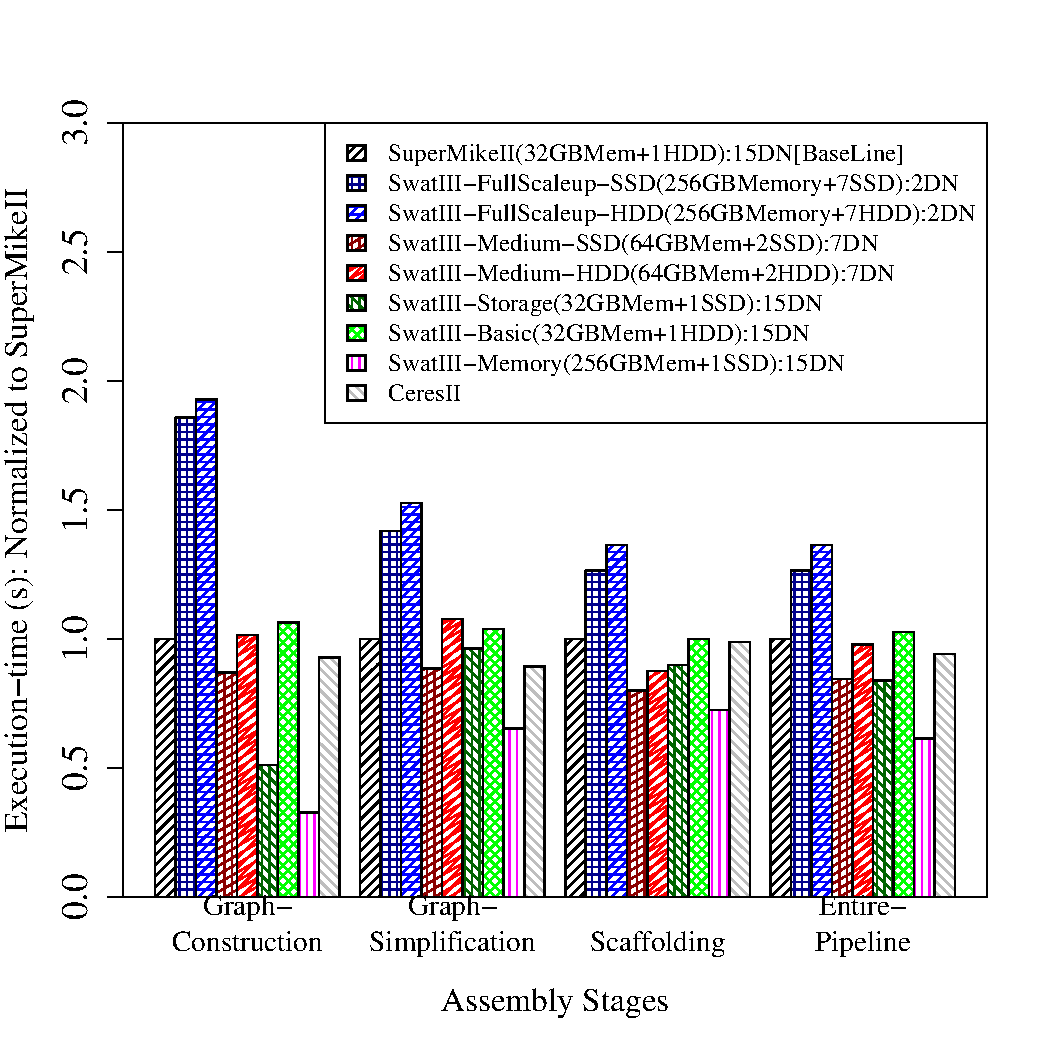
\includegraphics[width=\textwidth, height=.3\textheight]{Figure/PerormanceData/Plots/PerfDiffArch.pdf}
                \caption{Execution-time (Lower is better)}
                \label{fig:DifferentArchitecturesPerf}
        \end{subfigure}
        \begin{subfigure}[b]{0.5\textwidth}
                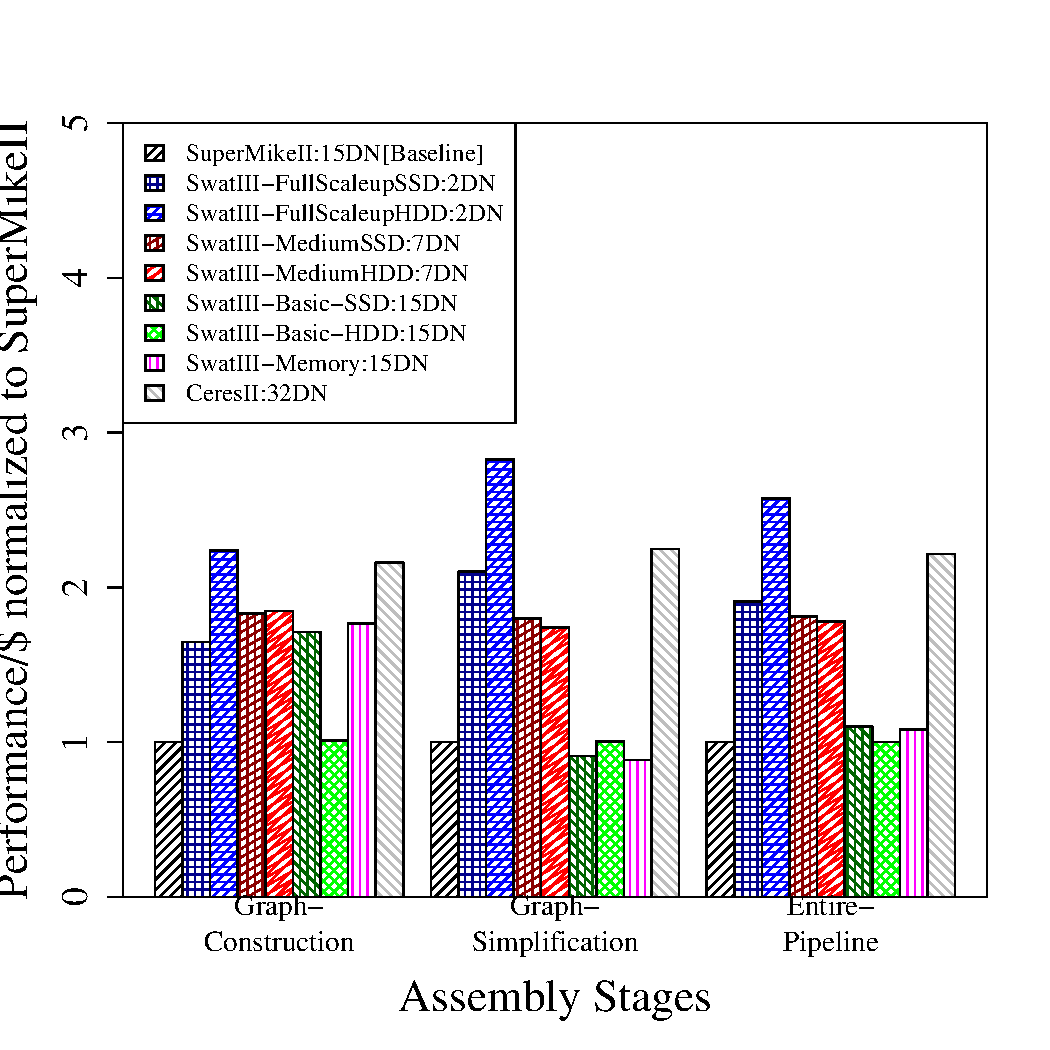
\includegraphics[width=\textwidth, height=.3\textheight]{Figure/PerormanceData/Plots/PerfPerDollarDiffArch.pdf}
                \caption{Performance/\$ (Higher is better)}
                \label{fig:DifferentArchitecturesPerfPerDollar}
        \end{subfigure}
        \caption{Compare different type of cluster architeture for bumble bee genome assembly pipeline}
  \label{fig:DifferentArchitectures}
\end{figure*}
In this section we compare the performance of different cluster architecture in terms of raw execution time as well as performance per dollar.
\subsection {Performance comparison of SuperMikeII and SwatIII with bumble bee genome}
Figure-\ref{fig:DifferentArchitecturesPerf} shows the relative merits of different cluster architecture in terms of raw execution time. The execution time is normalized to the baseline i.e. SuperMikeII.
Observe, we always keep the total aggregated storage and memory space almost same across all the clusters.
The basic assumption behind this experimental setup is that, the total amount of data should be held in its entirity in any of the cluster. 
Furthermore, the choice of the cluster in a cloud scenario is often driven by the sheer volume of the data rather than the performance.
%Since most of the time the selection of the clusters are driven by the sheer volume of data that needs some minimum storage and memory space to be analyzed, in our study, we did not compromise the total storage or memory space. All the clusters that we evaluate in this section has almost the same amount of total memory and storage space except SwatIII-Memory where the amount of memory is significantly higher than the others.
The observations are as follows:
1) The SwatIII-Memory, i.e. the 15-DataNode cluster with 256GB memory and one SSD per node performs the best in terms of raw execution time for any type of workload due to high resource availability.
2) Because of the io-bound nature of the Hadoop job, SSD shows better scalabality than HDD in the graph-construction stage with increase in number of nodes in the cluster, thus increasing the number of cores. There is almost no performance improvement in SwatIII-Medium-HDD (7-DN with 2-HDD each) and SwatIII-basic (15-DN with 1-HDD each). However, there is almost 50\% improvement in the corresponding SSD case (i.e. SwatIII-medium-SSD and SwatIII-Storage).
3) Number of cores plays a critical role in case of Giraph. We observed the optimum performance in graph simplification stage in SwatIII-Medium (8-nodes) cluster.
4) Although the use of SSD is beneficial for Hadoop when there is only one disk per node (as shown in SuperMikeII and SwatIII-Storage), in a full scaled-up environment with multiple disks per node, Hadoop shows similar performance with both HDD and SSD as shown in SwatIII-FullScaleup-SSD and SwatIII-FullScaleup-HDD.

\subsection {Performance to Price comparison between SuperMikeII and SwatIII variants with the bumble bee genome} \label{PriceToPerformance}
Table-\ref{table:PriceOfEachComponent} shows the cost\footnote{Price information is collected from http://www.newegg.com/ and http://www.amazon.com/} of each hardware component used in different clusters.
%It is worthy to mention here, We do not assume that a single scaled up server with one disk can accomodate the entire data.
%The total amount of data should be held in its entirity in the cluster for both scaled-up and scaled-out cases.
%Hence, we did not compromise with the total disk-space or memory-space required in case of scaled up and scaled out.
As mentioned earlier, the total aggregated storage and memory space is kept almost same across all the clusters except SwatIII-Memory which has a huge amount of total aggregated memory.
Which means, in our experiments, none of the cluster gets any price benefit over the other because of the total storage or memory space.   
Rather, we compare the performance to price from the view point of a proper architectural balance among number of cores, number of disks and amount of memory per node.
Since SuperMikeII resources are shared among many users whereas the SwatIII and CeresII are private cluster we did not consider the cost of network for a fair comparison.
Figure-\ref{fig:DifferentArchitecturesPerfPerDollar} shows the performance to price comparison among all the clusters.
The observations are as follows:
1) For a shuffle intensive Hadoop job, SuperMikeII and SwatIII-basic yields the lowest performance/\$ because of huge performance bottleneck caused by the io-wait.
2) Use of more memory per node as in SwatIII-Memory does not show any better result in terms of performance/\$ once SSD is used as underlying storage as in SwatIII-Storage for Hadoop.
3) Although the use of huge memory space in SwatIII-Memory shows the maximum performance in case of Giraph, it does not have much impact on performance/\$ when compared to low memory cluster (e.g. SwatIII-Storage or SwatIII-Basic) given the fact that, the graph fit in the total memory space.
%4) Hadoop yields almost similar performance to price for any number of nodes. This is because each core analyzes the same amount of data at a certain point of time (normally, determined by the hdfs block size).
5) For Giraph, the performance/\$ decreases almost linearly with the increase in the number of nodes. Whereas, Hadoop-performance/\$ shows very small variation with increasing the number of nodes, given there is no io-bottleneck (as in the SSD variant of SwatIII-FullScaleup-/Medium/Storage). 
This is because each computation-core analyzes the same amount of data at a certain point of time in case of Hadoop (determined by the HDFS block size), resulting in full CPU-utilization. Whereas, in a Giraph job, more the number of nodes less is the amount of data handled by each core at a certain point of time, thus improving the performance in the cost of lower CPU utilization.
%6) The scaffolding phase, the series of small Hadoop and Giraph jobs shows trhe similar trend as the Giraph only workflow because each involves very less amount of disk-io. 
\begin{table}
\begin{center}
	\begin{tabular}{ |p{5cm} | p{3cm} |} \hline
		Component & Cost (\$)\\ \hline
		Intel SandyBridge Xeon 64bit Ep series (8-cores): used in SuperMikeII and Each variant of SwatIII & 1520\\ \hline
		Intel Xeon E3-1220L V2 (2-cores): used in CeresII & 389\\ \hline
		1-HDD (Western Digital, 500GB ) & 67\\ \hline
		1-SSD (Samsung, 500GB) & 177\\ \hline
		Dell Poweredge 16GB meory module & 139\\ \hline
	\end{tabular}
	\caption{Cost of each hardware component}
	\label{table:PriceOfEachComponent}
\end{center}
\end{table}

\subsection {Comparing SuperMikeII and SwatIII with Large human-genome }
\begin{figure}[htb]
        \begin{subfigure}[b]{0.23\textwidth}
                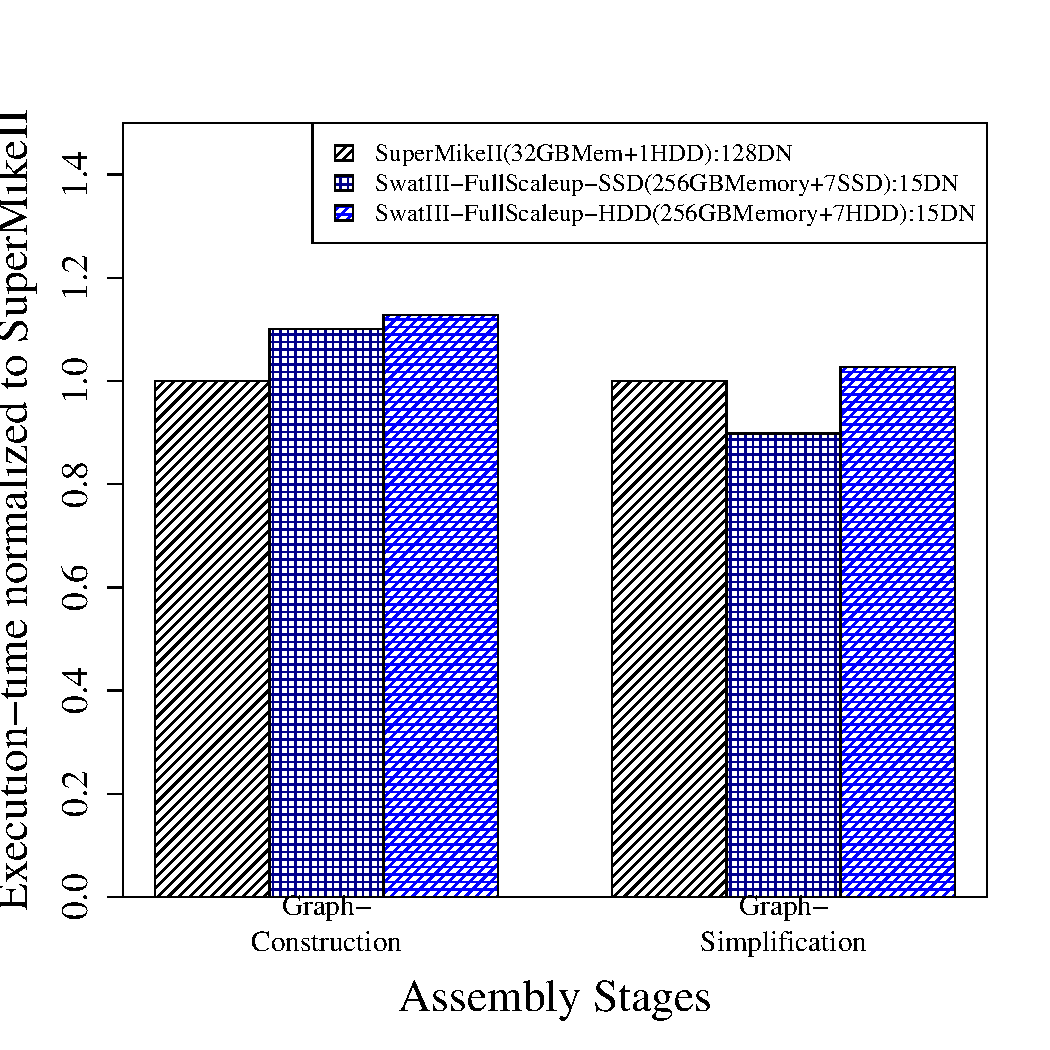
\includegraphics[width=\textwidth]{Figure/PerormanceData/Plots/PerfDiffArchHum.pdf}
                \caption{Execution-time (Lower is better)}
                \label{fig:DifferentArchitecturesPerfHum}
        \end{subfigure}
        \begin{subfigure}[b]{0.23\textwidth}
                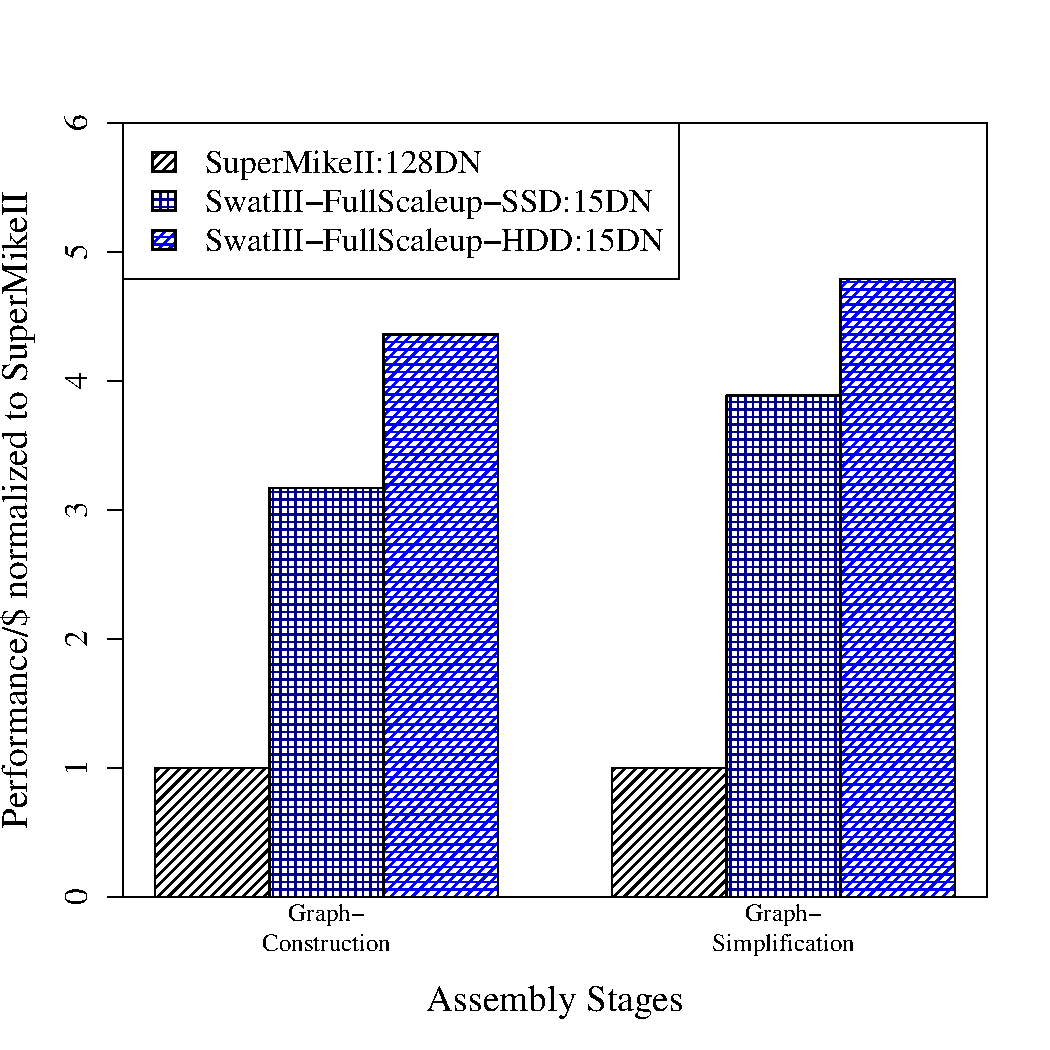
\includegraphics[width=\textwidth]{Figure/PerormanceData/Plots/PerfPerDollarDiffArchHum.pdf}
                \caption{Performance/\$ (Higher is better)}
                \label{fig:DifferentArchitecturesPerfPerDollarHum}
        \end{subfigure}
        \caption{Compare different type of cluster architeture for human genome assembly pipeline}
  \label{fig:DifferentArchitecturesHum}
\end{figure}  

In order to evaluate the cumulative impact of all the hardware components (i.e. network, cpu-cores, storage and memory) on the entire cluster we summarize our study with a stress testing of SuperMikeII and SwatIII clusters using the large scale 452GB human genome that produces 3.2TB of graph(refer to table-\ref{table:HumanData}).
In this part we utilize the maximum amount of resources that are available in any of the compute-clusters. 
We used 127-datanodes of SuperMikeII to accomodate the huge volume of data: either stored on disk (HDFS data or shuffled data) or the huge graph that is loaded in memory. 
On the other hand, we use 15-datanodes in the SwatIII-Full-Scaleup cluster (both HDD and SSD variant) which yields almost same amount of storage space as well as memory.
As mentioned before, due to the low value of maximum allowed file descriptor in SuperMikeII ($ulimit -n$ is set to 1024) we could not run the scaffolding stage in this cluster. Hence, remove it from the comparison.

Figure-\ref{fig:DifferentArchitecturesPerfHum} and \ref{fig:DifferentArchitecturesPerfPerDollarHum} shows the execution time and the performance/\$ respectively for the Hadoop-based graph-construction and Giraph-based graph-simplification stage of human genome assembly on three different cluster architectures.
The observations are as follows:
1) The 128nodes of SuperMikeII (2032-cores) shows only 15-17\% better performance than 15-datanodes of any variant of SwatIII-Full-Scaleup cluster (240 physical cores) while using almost 9-times more cores in the Hadoop-based graph-construction stage.
The reason behind the suboptimal performance in superMikeII is two folded: first, the huge amount of io-wait resulted by only one HDD per node as discussed in section-\ref{EffectOfSSD}. Second, the availability of less effective-network-bandwidth between compute-nodes because of resource sharing among many users as discussed in section-\ref{EffectOfNetwork}. However, Hadoop depends on network only once in the entire job: during data transfer tot he reducers
2) The Giraph-based graph-simplification stage performs 10\% better in SwatIII-FullScaleup-SSD than SuperMikeII. Since Giraph is more network intensive, the higher effective-network-bandwidth between compute-nodes of SwatIII yields better performance although it has very less amount of cores than SuperMikeII.
3) Both HDD and SSD variants of SwatIII-FullScaleup shows almost similar performance for both Hadoop and Giraph (less than 5\% variation). The effect is similar as discussed in section-\ref{ScaledupClusterAndSSD}.
4) In terms of performance/\$ any of the SwatIII-FullScaleup cluster is found to yield almost 4.5-times better result for the Hadoop stage and almost 5-times better result for the Giraph stage.

\subsection {Scaledup cluster and SSD} \label{ScaledupClusterAndSSD}
\begin{figure}[h]
  \centering
  \begin{subfigure}[b]{0.23\textwidth}
          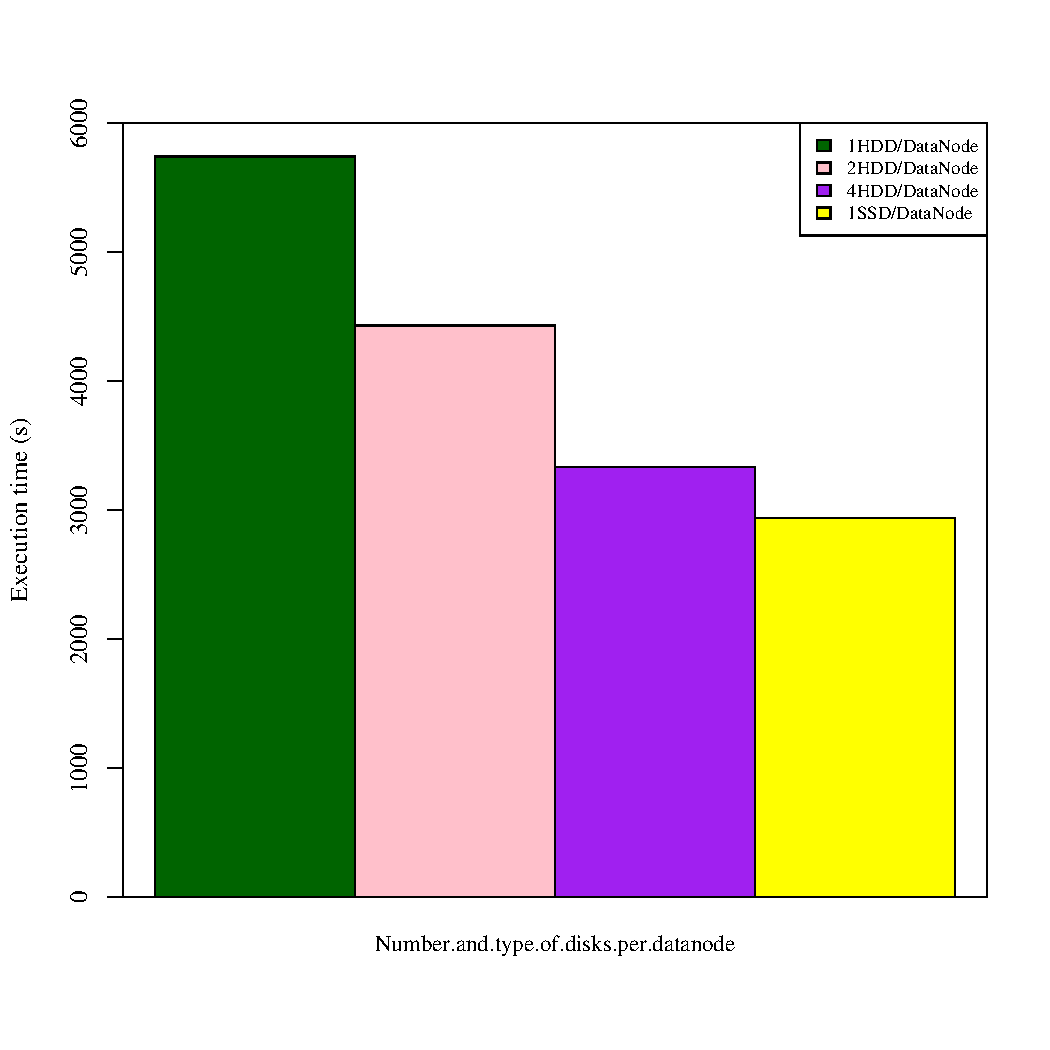
\includegraphics[width=\textwidth]{Figure/PerormanceData/Plots/SSDHDDSameNode.pdf}
          \caption{Performance trend using 1, 2 and 4 HDD(s) and 1-SSD per node using a 15 datanodes}
          \label{fig:SsdN4Hdd}
  \end{subfigure}
  \begin{subfigure}[b]{0.23\textwidth}
          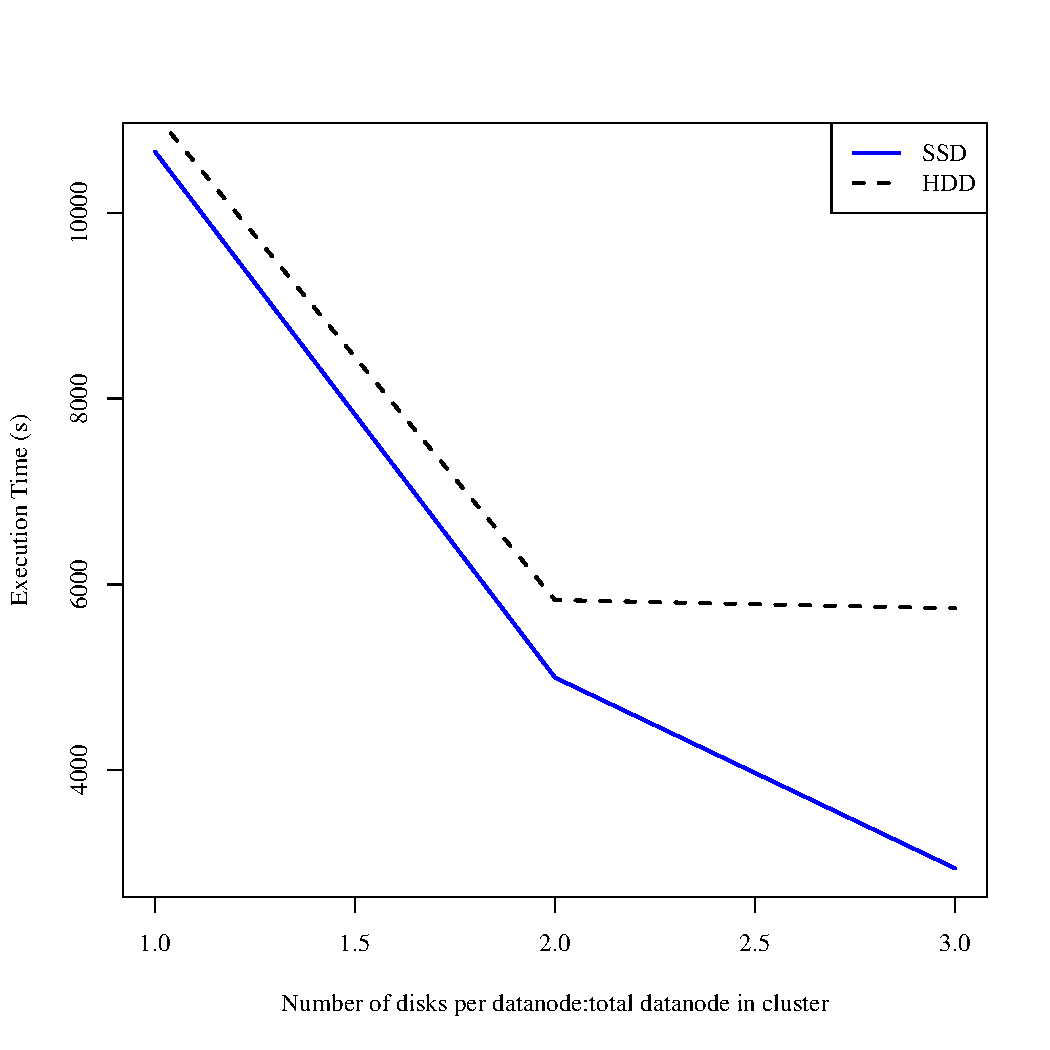
\includegraphics[width=\textwidth]{Figure/PerormanceData/Plots/SSDHDDDiffNode.pdf}
          \caption{Performance trend for SSD and HDD using 1, 2, 7 disks per node in 15, 7 and 2 datanodes}
          \label{fig:SsdNHddDiffNodes}
  \end{subfigure}
  \caption{Performance trend using HDD and SSD}
  \label{fig:SsdNHdd}
\end{figure}
Cloud service providers already started using SSDs as the elemental feature in their cloud infrastructure.
Furthermore, many of the available cloud instances provide more SSDs per compute-node in order to improve the performance.
Consequently, the setup-cost as well as the pricing of these scaledup instances increase.
For example AWS i2.8xlarge storage-optimized instance offers 8SSDs per compute-node with 32 v-cores per node in a rate of \$6.82 per hour which is one of the high-cost AWS-EC2-instances \footnote{http://aws.amazon.com/ec2/pricing/}.
In this section, we analyze how to leverage SSDs in a cost-effective manner.
In particular, we point out the scaledup scenario where HDDs and SSDs yield similar level of performance.

Figure-\ref{fig:SsdN4Hdd} compares the performance of a single SSD and  increasing number of HDDs per node for the Hadoop-based graph-construction stage of the bumble bee genome assembly pipeline.
The performance improves almost linearly by increasing the number of HDDs per node in the cluster.
On the other hand, 4-HDDs per node shows similar performance (only 5\% variation) with a single-SSD per node.
We did not observe any more significant improvement by providing more SSDs per node, concluding the disk-io rate reaches a saturation point.
As a consequence, we did not find any significant performance-difference between SwatIII-FullScaleup-SSD and -HDD as shown in figure-\ref{fig:SsdNHddDiffNodes} while assembling the same bumble bee genome using 2-datanodes each with 7-disks.
However, SSD shows significantly better performnce as well as scalability than HDD when we scale out by adding more compute nodes to the cluster (thus, increasing the total number of cores) and reducing the number of disks per node (thus, keeping the total storage space almost same in the cluster).

\subsection {CeresII: Samsung-MicroBricks for shared nothing paradigm} \label{CeresII:Scaledout-in-a-boxAndSSD}
%In the previous sections we observed that SSD shows huge performance benefit in a scaled out cluster setup where each node has fewer number of DAS.
%We also observed that the performance gap between HDD and SSD decreases with increase in number of DAS per node.
%Finally, depending upon the number of cores (and processor family) per node, beyond a certain threshold point HDD and SSD starts perform similarly.
%However, due to less number of cores in fewer nodes, the overall performance may drop significantly. On the other hand, use of more scaledup servers has an immidiate impact on performance to price.

In this section, we evaluate a Samsung-MicroBricks based novel prototype-architecture called CeresII which is an improvement over CeresI \cite{Cluster:ceres1}.
As mentioned before, CeresII uses 2 physical cores, 1 SSD and 16GB memory per computation module.
In order to assemble the 95GB bumblebee genome we use 32 such modules of this cluster as Hadoop-datanodes.
The last columns of different stages of the assembly in Figure-\ref{fig:DifferentArchitecturesPerf} shows the execution time of CeresII.
As it can be seen, CeresII performs almost similar in every stage of the assembly pipeline and shows almost 2-times improvement in performance/\$.
%On the other hand, CeresII shows similar Perf and Perf/\$ to this medium sized cluster(7DNs). Moreover, the MicroBrick architecture is expected to consume less power and obviously the space thus yielding more benefit in terms of TCO (total cost of ownership).
%Its performance is almost comparable to SwatIII-Medium-SSD which used 7-datanodes.

From the performance-study between SuperMikeII and SwatIII, we noticed a huge tradeoff between the execution time and the performance/\$. 
For example, the full-scaledup small-sized clusters (2-DNs cases), even though shows lower performance than the SuperMikeII-baseline, it shows a magnitude higher Perf/\$. Again, considering both performance and cost, we can say, the medium sized clusters (7-DNs) are well balanced.
On the other hand, CeresII shows similar performance both in terms of execution time as well as performance/\$ to the medium sized cluster(7DNs). Moreover, the Samsung MicroBricks based architecture is expected to consume less power and obviously occupies less space. Hence, CeresII shows more benefit in terms of TCO (total cost of ownership) among all the clusters.

%However, the entire cluster (all the 32 modules) takes significantly less space than 8 nodes of SwatIII-Medium-SSD, thus yielding significantly better performance per rack-unit.

%In the last section we discuss the benefit of SSD in bigdata processing in a supercomputing environment.
%Many cloud service providers has already started offering SSDs as an elemental hardware feature in their cloud infrastructure.
%Furthermore, to eleminate the io-bound nature of bigdata analytics jobs, many cloud instances offer more than one SSD per node.  
%For example, the storage-otimized AWS-i2.8Xlarge instance offers 8SSDs per node with 32 virtual cores.
%Although other works as well as our experience show the benefit of using SSDs in a scaled out HPC environment where each node in the compute cluster is equipped with fewer (typically 1) DAS, how much beneficial it is to use more SSDs in each node in a computation cluster?
%Undoubtedly, use of more SSDs per node incurs huge cost in setting up the entire infrastructure. 
%Hence, we found it important to investigate how to efficiently leverage SSDs in a cloud environment in a cost effective manner.

%In our previous experiments we showed that the use of SSD increases the number of IOPS per node which reduces the io-wait time of the job, thus reduce the over all execution time of a Hadoop job.
%On the other hand, the total IOPS of a compute node is directly proportional to the number of DAS (HDDs or SSDs both) to it. 
%That is, increasing the number of HDDS per node will also increase the IOPS, there by reduce the execution time until the job is io-bound.
%However, once the job is compute-bound (i.e. almost 100\% CPU-utilization with no io-wait) adding more disks or changing the storage media type to the compute node does not help in improving the prformance unless the number of processing cores is increased. 
%Hence, given a certain number of cores per node, in a compute-cluster with more disks attached per node, we expected a similar performance from both HDDs and SSDs beyond a certain number of disks.

%To better understand the impact of HDD and SSD in terms of number of IOPS, we started with evaluating the performance of a single SSD per node in the SwatIII-Storage cluster. 
%We replaced the single SSD used in each node of SwatIII-Storage with increasing number of HDDs and assembled the 95GB bumble-bee genome each time using 16nodes until the  execution time is similar to that of the single SSD case.
%Figure-\ref{fig:SsdN4Hdd} shows the execution time of different number of HDDs per node again normalized to the baseline.
%We observe almost a linear trend in performance improvement by increasing the number of HDDs per node in the cluster.
%We also observed, 4HDDs per node shows similar performance (only 6\% variation) with a single-SSD in the graph-construction phase.
%Hence, at this point, we expected a similar performance for both HDDs and SSDs with more than 4 DAS per node in any compute cluster with the same number of cores per node.
%\begin{figure}[h!]
%  \centering
%  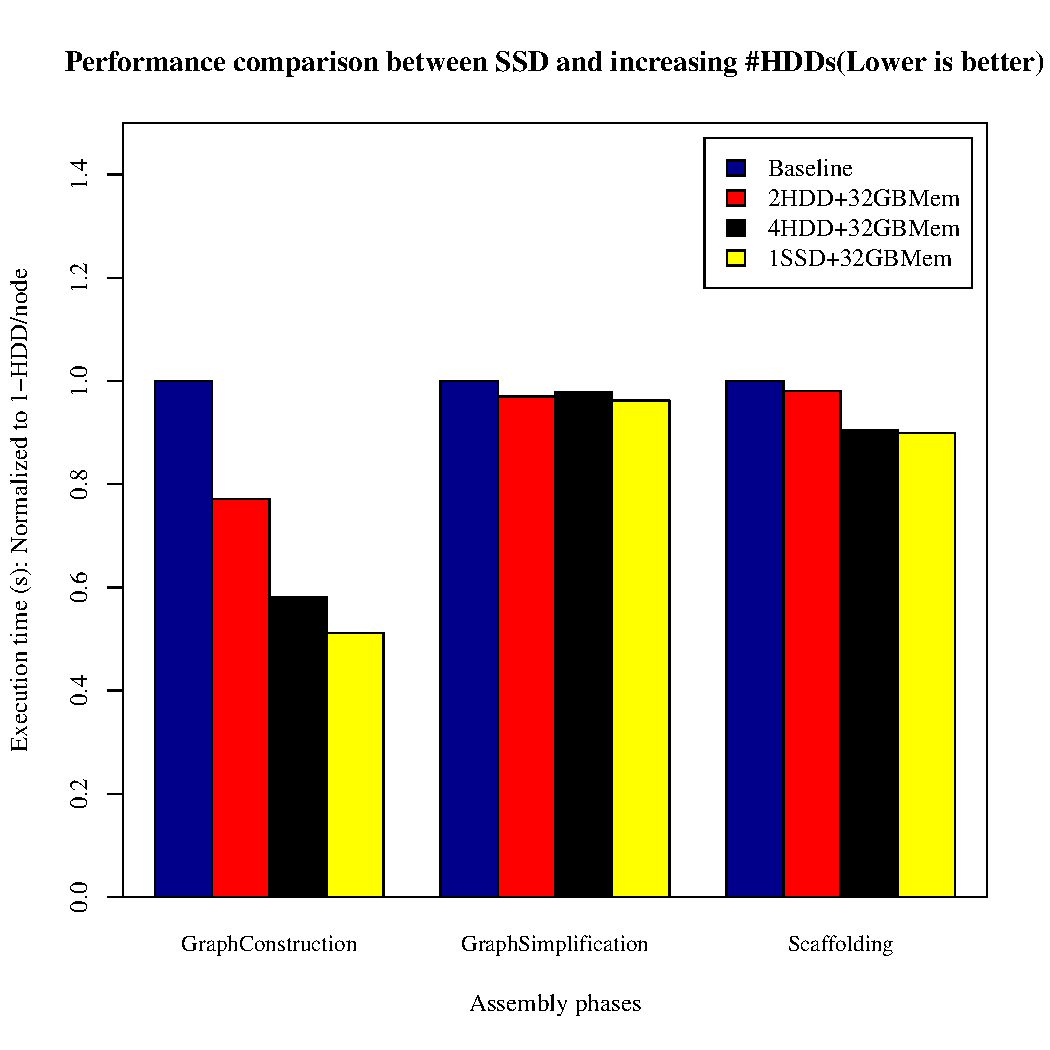
\includegraphics[width=0.5\textwidth]{Figure/PerormanceData/Plots/SSD4HDD.pdf}
%  \caption{Execution time of graph-construction phase using different number of HDDs and SSDs}
%  \label{fig:SsdN4Hdd}
%\end{figure}

%In order to substantiate our claim, in the next set of experiments, we scaled up 2 nodes of SwatIII for our tests in terms of storage and Memory.
%we added 7 storage disks to each node which yields almost the same storage space as in the SwatIII-Storage cluster.
%We also used 256GB RAM per node in order to get same amount of memory-space as in SwatIII-Storage.
%For the sake of convenience we named the scaled up clusters as SwatIII-FullScaleup-HDD and SwatIII-FullScaleup-SSD according to the storage type attached in each node.
%Figure-\ref{fig:SuperMikeSwatScaleUp} shows the execution time of each phase of our assembler.
%Observe, the HDD and the SSD both perform similarly in each phase of the assembler including the Hadoop-based shuffle-intensive graph-construction phase.
%Figure-iopsscaleup shows the similar number of io operations per second in case of both 7HDDs and 7SSDs throughout the assembly process which is the underlying reason behind the same level of performance.

%The above study helps the data scientists in choosing their cloud platforms in cost-effective manner. 
%The choice of the cloud instance is actually driven by two facts: 1) Minimum storage and memory space which can accomodate the data and 2) the perfromance.
%On the basis of our observation, we recommend the data scientists to use the following rule for a shuffle-intensive mapreduce job before choosing a cloud instance:
%If, 
%$ (TotalShuffledData / NumNodesInCluster)/ SingleDiskCapacity < ThresholdPoint $
%then, SSD is benefitial in terms of performance, where the $ThresholdPoint$ is determined by number of cores and the processor family. 
%Cloud-service providers should be aware of the $ThresholdPoint$ befor investing for their infrastructure. 
%In our case with (i.e. 16 vcores per node) the $ThresholdPoint$ is 4.

\section {Conclusion}
%The conclusion goes here.
%Despite of the fundamental differences in computation and communication characteristics involved in these two paradigms, the promising performance result of these state of the art bigdata analytics software on different distributed cyber infrastructure. 



% conference papers do not normally have an appendix


% use section* for acknowledgement
\section*{Acknowledgment}


The authors would like to thank...





% trigger a \newpage just before the given reference
% number - used to balance the columns on the last page
% adjust value as needed - may need to be readjusted if
% the document is modified later
%\IEEEtriggeratref{8}
% The "triggered" command can be changed if desired:
%\IEEEtriggercmd{\enlargethispage{-5in}}

% references section

% can use a bibliography generated by BibTeX as a .bbl file
% BibTeX documentation can be easily obtained at:
% http://www.ctan.org/tex-archive/biblio/bibtex/contrib/doc/
% The IEEEtran BibTeX style support page is at:
% http://www.michaelshell.org/tex/ieeetran/bibtex/
\bibliographystyle{IEEEtran}
% argument is your BibTeX string definitions and bibliography database(s)
\bibliography{bare_conf_bib}
%
% <OR> manually copy in the resultant .bbl file
% set second argument of \begin to the number of references
% (used to reserve space for the reference number labels box)
%\begin{thebibliography}{1}

%\end{thebibliography}

% that's all folks
\end{document}


